\documentclass{article}

% LOAD PREAMBLE
% The preamble is where settings and macros for the entire document reside.
% ~ ~ ~ ~ ~ ~ ~ ~ ~ ~ ~ ~ ~ ~ ~ ~ ~ ~ ~ ~ ~ ~ ~ ~ ~ ~ ~ ~ ~ ~ ~ ~ ~ ~ ~ ~ ~ ~ ~ ~ ~ ~ ~ ~ ~ ~ ~ ~

\usepackage[utf8]{inputenc}
\usepackage{amsmath}
\usepackage{amssymb} % for \mathbb
\usepackage{graphicx} % for figures
\usepackage{color}
\usepackage[usenames,dvipsnames]{xcolor}
\usepackage{hyperref} % for hyperlinks
\usepackage{float} % for figures
% ~ ~ ~ ~ ~ ~ ~ ~ ~ ~ ~ ~ ~ ~ ~ ~ ~ ~ ~ ~ ~ ~ ~ ~ ~ ~ ~ ~ ~ ~ ~ ~ ~ ~ ~ ~ ~ ~ ~ ~ ~ ~ ~ ~ ~ ~ ~ ~
% CUSTOM COLOUR
\definecolor{DGrey}{rgb}{0.1,0.1,0.1} % Dark Grey
% ~ ~ ~ ~ ~ ~ ~ ~ ~ ~ ~ ~ ~ ~ ~ ~ ~ ~ ~ ~ ~ ~ ~ ~ ~ ~ ~ ~ ~ ~ ~ ~ ~ ~ ~ ~ ~ ~ ~ ~ ~ ~ ~ ~ ~ ~ ~ ~
\title{ Introduction to Engineering Written Assignment Questions}
\date{January 2013}
\author{Greg Mayer and Daniel Connelly}
% ~ ~ ~ ~ ~ ~ ~ ~ ~ ~ ~ ~ ~ ~ ~ ~ ~ ~ ~ ~ ~ ~ ~ ~ ~ ~ ~ ~ ~ ~ ~ ~ ~ ~ ~ ~ ~ ~ ~ ~ ~ ~ ~ ~ ~ ~ ~ ~
% HEADER/FOOTER
\usepackage{fancyheadings}
\pagestyle{myheadings} % set headings to be user defined
\fancyhead{} % To create custom header, clear default layout
\renewcommand{\subsectionmark}[1]{\markright{{\color{DGrey}\thesubsection} \ {\color{DGrey}#1}}}
\fancyhead[LE,LO]{\subsectionmark} % To create custom header, clear default layout

% ~ ~ ~ ~ ~ ~ ~ ~ ~ ~ ~ ~ ~ ~ ~ ~ ~ ~ ~ ~ ~ ~ ~ ~ ~ ~ ~ ~ ~ ~ ~ ~ ~ ~ ~ ~ ~ ~ ~ ~ ~ ~ ~ ~ ~ ~ ~ ~
% ENUMERATION

\usepackage{enumitem}   % so that question numbers can be formatted 
\setenumerate[1]{label=\thesubsection.\arabic*.} % enumerate environment: add section numbers to items
% ~ ~ ~ ~ ~ ~ ~ ~ ~ ~ ~ ~ ~ ~ ~ ~ ~ ~ ~ ~ ~ ~ ~ ~ ~ ~ ~ ~ ~ ~ ~ ~ ~ ~ ~ ~ ~ ~ ~ ~ ~ ~ ~ ~ ~ ~ ~ ~
% MARGINS
\usepackage{anysize}
\marginsize{2.5cm}{2.5cm}{1cm}{1cm}
% ~ ~ ~ ~ ~ ~ ~ ~ ~ ~ ~ ~ ~ ~ ~ ~ ~ ~ ~ ~ ~ ~ ~ ~ ~ ~ ~ ~ ~ ~ ~ ~ ~ ~ ~ ~ ~ ~ ~ ~ ~ ~ ~ ~ ~ ~ ~ ~
% PAGE NUMBERING
\pagenumbering{arabic}
% ~ ~ ~ ~ ~ ~ ~ ~ ~ ~ ~ ~ ~ ~ ~ ~ ~ ~ ~ ~ ~ ~ ~ ~ ~ ~ ~ ~ ~ ~ ~ ~ ~ ~ ~ ~ ~ ~ ~ ~ ~ ~ ~ ~ ~ ~ ~ ~
% Custom Commands
\newcommand{\Emph}[1]{\textbf{#1}} % Emphasize
\newcommand{\R}{\mathbb{R}} 
\newcommand{\BM}{\begin{bmatrix}} % Begin Matrix
\newcommand{\EM}{\end{bmatrix}} % End Matrix
\newcommand{\BEN}{\begin{enumerate}[leftmargin=1.1cm]}% Begin ENumerate
\newcommand{\EEN}{\end{enumerate}} % End ENumerate
\newcommand{\MB}{\mathbf} % Math Bold

\newcommand{\px}{\frac{\partial}{\partial x}} % Partial wrt x
\newcommand{\py}{\frac{\partial}{\partial y}} % Partial wrt y

\newcommand{\pfx}{\frac{\partial f}{\partial x}} % Partial of f wrt x
\newcommand{\pfy}{\frac{\partial f}{\partial y}} % Partial of f wrt y
\newcommand{\pfxy}{\frac{\partial^2 f}{\partial y \partial x}} % Partial of f wrt y
\newcommand{\pfyx}{\frac{\partial^2 f}{\partial x \partial y}} % Partial of f wrt y

\newcommand{\ux}{\frac{\partial u}{\partial x }} % Partial of u wrt x
\newcommand{\uk}{\frac{\partial u}{\partial k }} % Partial of u wrt k
\newcommand{\ut}{\frac{\partial u}{\partial t}} % Partial of u wrt t
\newcommand{\utt}{\frac{\partial^2u}{\partial t^2}} % Partial of u wrt t
\newcommand{\us}{\frac{\partial u}{\partial s}} % Partial of u wrt t
\newcommand{\uss}{\frac{\partial^2 u}{\partial s^2}} % Partial of u wrt t
\newcommand{\kx}{\frac{\partial k}{\partial x }} % Partial of k wrt x
\newcommand{\kt}{\frac{\partial k}{\partial t }} % Partial of k wrt t

\newcommand{\pxu}{\frac{\partial x}{\partial u}} % x wrt u
\newcommand{\pxv}{\frac{\partial x}{\partial v}} % x wrt v
\newcommand{\pxw}{\frac{\partial x}{\partial w}} % x wrt v
\newcommand{\pxt}{\frac{\partial x}{\partial t}} % x wrt t
\newcommand{\pyu}{\frac{\partial y}{\partial u}} % y wrt u
\newcommand{\pyv}{\frac{\partial y}{\partial v}} % y wrt v
\newcommand{\pyw}{\frac{\partial y}{\partial w}} % y wrt v
\newcommand{\pyt}{\frac{\partial y}{\partial t}} % y wrt t
\newcommand{\pzu}{\frac{\partial z}{\partial u}} % z wrt u
\newcommand{\pzv}{\frac{\partial z}{\partial v}} % z wrt v
\newcommand{\pzw}{\frac{\partial z}{\partial w}} % z wrt v
\newcommand{\pzt}{\frac{\partial z}{\partial t}} % z wrt t


\newcommand{\VCT}{\textit{Vector Calculus} by Michael Corral} % Vector Calculus Textbook
\newcommand{\CAT}{\textit{College Algebra} by Carl Stitz and Jeff Zeager} % College Algebra Textbook
\newcommand{\From}{The following questions are related to } % Questions ....
% ~ ~ ~ ~ ~ ~ ~ ~ ~ ~ ~ ~ ~ ~ ~ ~ ~ ~ ~ ~ ~ ~ ~ ~ ~ ~ ~ ~ ~ ~ ~ ~ ~ ~ ~ ~ ~ ~ ~ ~ ~ ~ ~ ~ ~ ~ ~ ~
% ONLY USED FOR EDITING
\newcommand{\rednote}[1]{{\color{red}\textit{\textbf{#1}}}} % Shortcut for formatting notes for developers
\newcommand{\FromC}[1]{{\color{DGrey}\textit{#1}}} % Shortcut for coloring the "from" text
% ~ ~ ~ ~ ~ ~ ~ ~ ~ ~ ~ ~ ~ ~ ~ ~ ~ ~ ~ ~ ~ ~ ~ ~ ~ ~ ~ ~ ~ ~ ~ ~ ~ ~ ~ ~ ~ ~ ~ ~ ~ ~ ~ ~ ~ ~ ~ ~
% AUGMENTED MATRIX MACRO
% thanks to http://tex.stackexchange.com/questions/2233/whats-the-best-way-make-an-augmented-coefficient-matrix
\newenvironment{amatrix}[1]{%
  \left[\begin{array}{@{}*{#1}{c}|c@{}}
}{%
  \end{array}\right]
}
% ~ ~ ~ ~ ~ ~ ~ ~ ~ ~ ~ ~ ~ ~ ~ ~ ~ ~ ~ ~ ~ ~ ~ ~ ~ ~ ~ ~ ~ ~ ~ ~ ~ ~ ~ ~ ~ ~ ~ ~ ~ ~ ~ ~ ~ ~ ~ ~
% PAGE LAYOUT
\addtolength{\topmargin}{10pt}
\addtolength{\headsep}{10pt}
\addtolength{\textheight}{-20pt}


% ~~~~~~~~~~~~~~~~~~~~~~~~~~~~~~~~~~
\begin{document}
\maketitle
\tableofcontents

\rednote{Note: hyperlinks in Part II of table of contents are kinda broken. Perhaps we should create two documents: Questions and Solutions. Or try using a different document class.}

\newpage
% ~~~~~~~~~~~~~~~~~~~~~~~~~~~~~~~~~~
% QUESTIONS
\part{Questions for Written Assignments}
\setcounter{section}{1}
% ~  ~  ~  ~  ~  ~  ~  ~  ~  ~  ~  ~  ~  ~  ~  ~  ~  ~  ~  ~  ~  ~  ~  ~
\section{Multivariable Functions and Algebra}
% ~  ~  ~  ~  ~  ~  ~  ~  ~  ~  ~  ~  ~  ~  ~  ~  ~  ~  ~  ~  ~  ~  ~  ~
\subsection{Dot Products and Cross Products}

\FromC{\From sections 1.3 and 1.4 of \VCT.}

\BEN 

\item % QUESTION 
Find two unit vectors perpendicular to vectors $\begin{bmatrix} 1 \\ 0\\4 \end{bmatrix}$ and $\mathbf{i}-2\mathbf{j}+\mathbf{k}$. 
% -  -  -  -  -  -  -  -  -  -  -  -  -  -  -  -  -  -  -  -  -  -  -  -  -  -  -  -  -  -  
\item 
Suppose vectors $\mathbf{a}$, $\mathbf{b}$, and $\mathbf{c}$ are in $\mathbb{R}^3$, and \textbf{a}$\ne 0$. If \textbf{a}$\cdot\mathbf{b}=\mathbf{a}\cdot\mathbf{c}$, does it follow that $\mathbf{b}=\mathbf{c}$? Briefly explain your answer. 

% -  -  -  -  -  -  -  -  -  -  -  -  -  -  -  -  -  -  -  -  -  -  -  -  -  -  -  -  -  -  
\item % QUESTION 
Consider the following vectors in $\R^2$:
\begin{align*}
\mathbf{a} = \begin{bmatrix} 1/\sqrt{2} \\ -1/\sqrt{2} \end{bmatrix}, \quad
\mathbf{b} = \begin{bmatrix} 1/\sqrt{2} \\ 1/\sqrt{2} \end{bmatrix}, \quad
\mathbf{r} =  \begin{bmatrix} 3 \\ 1 \end{bmatrix}.
\end{align*}
\begin{enumerate}
\item Verify that $\mathbf{a}$ and $\mathbf{b}$ are perpendicular unit vectors. 
\item Use your results from part (a) to find constants $C_1$ and $C_2$ so that $\mathbf{r}=C_1\mathbf{a}+C_2\mathbf{b}$.
\end{enumerate}
% -  -  -  -  -  -  -  -  -  -  -  -  -  -  -  -  -  -  -  -  -  -  -  -  -  -  -  -  -  -  
\item % QUESTION 
Suppose that $\mathbf{a}$, $\mathbf{b}$ and $\mathbf{c}$ are nonzero vectors in $\R^3$. Prove the following statements.
\begin{enumerate}
\item If $||\mathbf{a} + \mathbf{b}||^2 = ||\mathbf{a}||^2 + ||\mathbf{b}||^2$, then vectors $\mathbf{a}$ and $\mathbf{b}$ are perpendicular. 
\item If $\mathbf{a}\times\mathbf{b} = \mathbf{a}\times\mathbf{c}$ and $\mathbf{a}\cdot\mathbf{b} = \mathbf{a}\cdot\mathbf{c}$, then $\mathbf{b} =\mathbf{c}$.
\end{enumerate}
% -  -  -  -  -  -  -  -  -  -  -  -  -  -  -  -  -  -  -  -  -  -  -  -  -  -  -  -  -  -  
\item 
Suppose that $\mathbf{a}$, $\mathbf{b}$ and $\mathbf{c}$ are nonzero vectors in $\R^3$. Identify which of the following statements are meaningless and which statements are not meaningless. Explain your reasoning.
\begin{enumerate}
\item  $\mathbf{a}\cdot (\mathbf{b} \times \mathbf{c})$ 
\item  $\mathbf{a}\cdot (\mathbf{b} \cdot \mathbf{c})$ 
\item  $\mathbf{a}\times (\mathbf{b} \cdot \mathbf{c})$ 
\item  $\mathbf{a}\times (\mathbf{b} \times \mathbf{c})$ 
\end{enumerate}
% -  -  -  -  -  -  -  -  -  -  -  -  -  -  -  -  -  -  -  -  -  -  -  -  -  -  -  -  -  -  
\item \textbf{Application to Mechanics} \\
Torque plays a fundamental role in many branches of engineering. It is vector that describes rotation rotation about a point or axis due to an applied force. If you haven't yet encountered torque, its mathematical definition is straightforward:
\begin{quote}
The torque, $\boldsymbol\tau$, about a pivot point $P$, that is produced by a force \textbf{F} applied at a point $Q$, is defined as $\boldsymbol\tau = \mathbf{r} \times \mathbf{F}$, where $\mathbf{r}=\overrightarrow{PQ}$.
\end{quote}
Torque is a vector that is produced by an applied force. For example, suppose that a force $\MB{F}=\frac{1}{2}\MB{i} + 0\MB{j} + 0\MB{k}$ is applied at the point $(1,C,0)$, about the pivot point (1,0,0), where $C\in\R$ is a constant. The resulting torque is simply 
\begin{align*}
\boldsymbol\tau =   
\begin{vmatrix}
   \MB{i} &  \MB{j} &  \MB{k} \\
   1-1 &  C-0 &  0 \\
   0.5 & 0 &  0 \\
  \end{vmatrix}=-\frac{C}{2}\MB{k}
\end{align*} 
A plot of the applied force and produced torque vectors is shown in Figure \ref{FigTorque}.
\begin{figure}[H]
  \begin{center}
    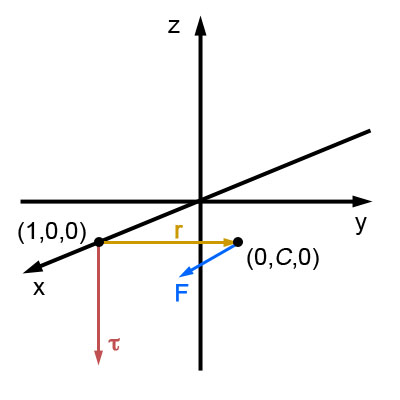
\includegraphics[width=0.5\textwidth]{ImgTorqueExample.jpg}
          \caption{\small{The torque, $\boldsymbol\tau$, about the pivot point (1,0,0), is produced by the applied force $\MB{F}$.\label{FigTorque} }}
  \end{center}
\end{figure}

Note that the magnitude of the torque vector is $||\boldsymbol\tau|| = C/2$, and that if we increase the value of $C$, two things happen: the applied force moves further away from the pivot point, and the magnitude of the produced torque increases. \\\\
% Consider that:
%\begin{itemize}
%\item intuitively, it is easier to rotate a screwdriver with a \textbf{large} handle than it is to rotate a screwdriver a small handle. If the 
%\item It is easier to spin a large wheel by pushing on its edge, rather than pushing on some point in the middle of the wheel. Moreover, we 
%\end{itemize}
\textbf{Units}\\
When \textbf{F} has units of Newtons (N), and $\MB{r}$ has units of meters (m), torque has units of $\text{N}\cdot\text{m}$.\\\\
\textbf{A Mechanics Problem}\\
Suppose that a bicycle has pedal arms that are 0.14 m long, and that a constant downward force of $100 \text{ N}$ is applied by a cyclist on one pedal.  Let $\theta \in [0,360^{\circ})$ be the angle between the vertical and the pedal arm, as shown in Figure \ref{FigCycle}. 
\begin{figure}[H]
  \begin{center}
    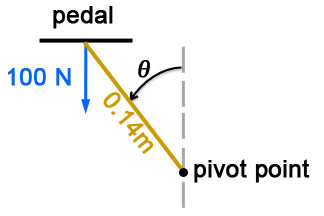
\includegraphics[width=0.4\textwidth]{ImgBicycle.jpg}
      \caption{\small{The pedal arm (orange) rotates about the pivot point. The angle it makes with the vertical direction is $\theta$, measured counter-clockwise. A constant downward force of 100 N is applied to the pedal, which is attached to the other end of the pedal arm.\label{FigCycle} }}
  \end{center}
\end{figure}
\BEN
  \item Determine the magnitude of the torque about the pivot point when $\theta$ is $30^{\circ}$ and when $\theta$ is $90^{\circ}$. Your answers should include the units of measurement. 
  \item Determine the magnitude of the torque about the pivot point for any $\theta$. Your answer should be a function of $\theta$.  
  \item What value(s) of $\theta$ minimize the produced torque? Briefly explain why. You should not need to compute any derivatives to answer this question. 
\EEN
Naturally, the torque vector can also be a function of time. In our bicycle example, the torque that is produced by the cyclist could change continuously as the pedal rotates about the pivot point. We will revisit the concept of torque as a vector function in a later assignment, after we have defined vector functions and their derivatives. 

% ~~~~~~~~~~~~~~~~~~~~~~~~~~~~~~~~~~~~~~~~~~~~~~~~~~~~~~~~~
\item % DETERMINANTS QUESTION 
Find all values of $x$ that satisfy the following equations.
\begin{enumerate}
\item \(
 \begin{vmatrix}
  3 &  2 &  0 \\
  1 &  x &  0 \\
  7 & -3 &  4
 \end{vmatrix} = 4.
\)
\item \(
 \begin{vmatrix}
  x & 1 \\
  4 & 4x
 \end{vmatrix} = \begin{vmatrix}
  -x & -2 \\
  2 & 2x + 8
 \end{vmatrix}
\).
\end{enumerate}
\EEN
\newpage % Page Break
% ~  ~  ~  ~  ~  ~  ~  ~  ~  ~  ~  ~  ~  ~  ~  ~  ~  ~  ~  ~  ~  ~  ~  ~
\subsection{Lines and Planes}

\purple{\From Section 1.5 of \VCT.}

\BEN
\item 
Find vector equations for the following lines.
\begin{enumerate}
\item Find the vector equation for the line that passes through the points (-1,2,1), and (3,-2,1).
\item Find the vector equation for the line that has parametric equations $x=2+2t, y=9t, z=5+t$.
\end{enumerate}
% -  -  -  -  -  -  -  -  -  -  -  -  -  -  -  -  -  -  -  -  -  -  -  -  -  -  -  -  -  -  
\item 
Calculate the following angles.
\begin{enumerate}
\item Calculate the angle between the vectors $\BM -1\\ 0 \\ 1 \EM$, and $\BM 0 \\ -2 \\ 2 \EM$.
\item Calculate the angle between the vector $\mathbf{x}=\BM 1 \\ 0 \\ 2 \EM$ and the plane $2x+y-z=0$.
\end{enumerate}
% -  -  -  -  -  -  -  -  -  -  -  -  -  -  -  -  -  -  -  -  -  -  -  -  -  -  -  -  -  -  
\item 
\Emph{Distance Between a Point and a Line}\\
Find the distance between the point (1,0,0) and the line $x=1, y=t, z=1$.
% -  -  -  -  -  -  -  -  -  -  -  -  -  -  -  -  -  -  -  -  -  -  -  -  -  -  -  -  -  -  
\item 
\Emph{Distance Between a Point and a Plane}\\
Consider the point $(-1,C,1)$ and the plane $2x+y-z=3$, where $C$ is an unknown constant. Find all possible values of $C$ such that the distance between the given point and plane is equal to $\sqrt{6}$. 
% -  -  -  -  -  -  -  -  -  -  -  -  -  -  -  -  -  -  -  -  -  -  -  -  -  -  -  -  -  -  
\item 
Consider the points $P, Q, R$ \\
\begin{align*}
P &=(1,0,3)\\
Q &=(2,2,3)\\
R &=(0,0,-1)
\end{align*}
\begin{enumerate}
\item Find a vector that is perpendicular to the plane that passes through these points.
\item Find the area of the triangle $\bigtriangleup PQR$.
\item Find a point $S$ so that a unique plane that passes through $P, Q$, and $S$ cannot be found. Describe why you cannot find a unique plane that passes through $P, Q$, and $S$. 
\end{enumerate}
%% -  -  -  -  -  -  -  -  -  -  -  -  -  -  -  -  -  -  -  -  -  -  -  -  -  -  -  -  -  -  
%\item % QUESTION 
%Find two unit vectors perpendicular to vectors $\begin{bmatrix} 1 \\ 0\\4 \end{bmatrix}$ and $\mathbf{i}-2\mathbf{j}+\mathbf{k}$. 
%% -  -  -  -  -  -  -  -  -  -  -  -  -  -  -  -  -  -  -  -  -  -  -  -  -  -  -  -  -  -  
%\item 
%Suppose vectors $\mathbf{a}$, $\mathbf{b}$, and $\mathbf{c}$ are in $\mathbb{R}^3$, and \textbf{a}$\ne 0$. If \textbf{a}$\cdot\mathbf{b}=\mathbf{a}\cdot\mathbf{c}$, does it follow that $\mathbf{b}=\mathbf{c}$? Briefly explain your answer. 
% -  -  -  -  -  -  -  -  -  -  -  -  -  -  -  -  -  -  -  -  -  -  -  -  -  -  -  -  -  -  
\item % EQUATIONS OF PLANES 
\Emph{Equations of Planes}\\
Find the equation of the plane that
\begin{enumerate}
\item passes through the points (-1,2,1), (3,-2,1), and (-1,1,-1).
\item passes through the point (-1,2,1) and contains the line $x=y=z$.
\end{enumerate}
% -  -  -  -  -  -  -  -  -  -  -  -  -  -  -  -  -  -  -  -  -  -  -  -  -  -  -  -  -  -  
\item % QUESTION 
Suppose we have two planes $2x+y-z=3$ and $x+3y+z=0$. Find the line of intersection between these two planes, and find the equation of the plane that passes through the line of intersection and through the point $(0,0,0)$.
% -  -  -  -  -  -  -  -  -  -  -  -  -  -  -  -  -  -  -  -  -  -  -  -  -  -  -  -  -  -  
\item % QUESTION
Suppose that $L_1$ is a line in $\R^3$.
\begin{enumerate}
\item Is it possible to find another line, $L_2$, that is parallel $L_1$, and intersects $L_1$ at only one point? Show that it is  possible, or show that it is not possible with a counterexample.
\item Suppose that there is a line $L_3$ that is is parallel to $L_1$, and that a plane $P$ includes both $L_1$ and $L_3$. Is it always true that there exists a plane that is perpendicular to $P$? 
\end{enumerate}
% -  -  -  -  -  -  -  -  -  -  -  -  -  -  -  -  -  -  -  -  -  -  -  -  -  -  -  -  -  -  
%\item % QUESTION 
%Consider the following vectors in $\R^2$:
%\begin{align*}
%\mathbf{a} = \begin{bmatrix} 1/\sqrt{2} \\ -1/\sqrt{2} \end{bmatrix}, \quad
%\mathbf{b} = \begin{bmatrix} 1/\sqrt{2} \\ 1/\sqrt{2} \end{bmatrix}, \quad
%\mathbf{r} =  \begin{bmatrix} 3 \\ 1 \end{bmatrix}.
%\end{align*}
%\begin{enumerate}
%\item Verify that $\mathbf{a}$ and $\mathbf{b}$ are perpendicular unit vectors. 
%\item Use your results from part (a) to find constants $C_1$ and $C_2$ so that $\mathbf{r}=C_1\mathbf{a}+C_2\mathbf{b}$.
%\end{enumerate}
%% -  -  -  -  -  -  -  -  -  -  -  -  -  -  -  -  -  -  -  -  -  -  -  -  -  -  -  -  -  -  
%\item % QUESTION 
%Suppose that $\mathbf{a}$, $\mathbf{b}$ and $\mathbf{c}$ are nonzero vectors in $\R^3$. Prove the following statements.
%\begin{enumerate}
%\item If $||\mathbf{a} + \mathbf{b}||^2 = ||\mathbf{a}||^2 + ||\mathbf{b}||^2$, then vectors $\mathbf{a}$ and $\mathbf{b}$ are perpendicular. 
%\item If $\mathbf{a}\times\mathbf{b} = \mathbf{a}\times\mathbf{c}$ and $\mathbf{a}\cdot\mathbf{b} = \mathbf{a}\cdot\mathbf{c}$, then $\mathbf{b} =\mathbf{c}$.
%\end{enumerate}
%% -  -  -  -  -  -  -  -  -  -  -  -  -  -  -  -  -  -  -  -  -  -  -  -  -  -  -  -  -  -  
%\item 
%Suppose that $\mathbf{a}$, $\mathbf{b}$ and $\mathbf{c}$ are nonzero vectors in $\R^3$. Identify which of the following statements are meaningless and which statements are not meaningless. Explain your reasoning.
%\begin{enumerate}
%\item  $\mathbf{a}\cdot (\mathbf{b} \times \mathbf{c})$ 
%\item  $\mathbf{a}\cdot (\mathbf{b} \cdot \mathbf{c})$ 
%\item  $\mathbf{a}\times (\mathbf{b} \cdot \mathbf{c})$ 
%\item  $\mathbf{a}\times (\mathbf{b} \times \mathbf{c})$ 
%\end{enumerate}
%% -  -  -  -  -  -  -  -  -  -  -  -  -  -  -  -  -  -  -  -  -  -  -  -  -  -  -  -  -  -  
%\item \textbf{Application to Mechanics, Part I} \\
%Torque plays a fundamental role in many branches of engineering. It is vector that describes rotation rotation about a point or axis due to an applied force. If you haven't yet encountered torque, its mathematical definition is straightforward:
%\begin{quote}
%The torque, $\boldsymbol\tau$, about a pivot point $P$, that is produced by a force \textbf{F} applied at a point $Q$, is defined as $\boldsymbol\tau = \mathbf{r} \times \mathbf{F}$, where $\mathbf{r}=\overrightarrow{PQ}$.
%\end{quote}
%Torque is a vector that is produced by an applied force. For example, suppose that a force $\MB{F}=\frac{1}{2}\MB{i} + 0\MB{j} + 0\MB{k}$ is applied at the point $(1,C,0)$, about the pivot point (1,0,0), where $C\in\R$ is a constant. The resulting torque is simply 
%\begin{align*}
%\boldsymbol\tau =   
%\begin{vmatrix}
%   \MB{i} &  \MB{j} &  \MB{k} \\
%   1-1 &  C-0 &  0 \\
%   0.5 & 0 &  0 \\
%  \end{vmatrix}=-\frac{C}{2}\MB{k}
%\end{align*} 
%A plot of the applied force and produced torque vectors is shown below.
%\begin{figure}[!htbp]
%  \begin{center}
%    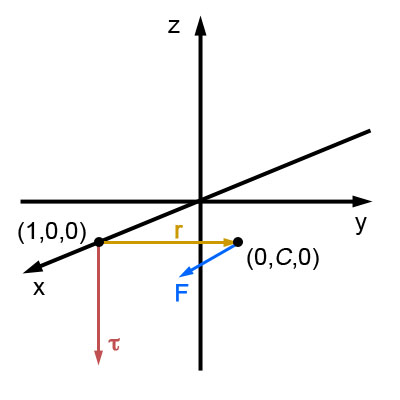
\includegraphics[width=0.5\textwidth]{ImgTorqueExample.jpg}
%  \end{center}
%\end{figure}
%
%Note that the magnitude of the torque vector is $||\boldsymbol\tau|| = C/2$, and that if we increase the value of $C$, two things happen: the applied force moves further away from the pivot point, and the magnitude of the produced torque increases. \\\\
%% Consider that:
%%\begin{itemize}
%%\item intuitively, it is easier to rotate a screwdriver with a \textbf{large} handle than it is to rotate a screwdriver a small handle. If the 
%%\item It is easier to spin a large wheel by pushing on its edge, rather than pushing on some point in the middle of the wheel. Moreover, we 
%%\end{itemize}
%\textbf{Units}\\
%When \textbf{F} has units of Newtons (N), and $\MB{r}$ has units of meters (m), torque has units of $\text{N}\cdot\text{m}$.\\\\
%\textbf{Questions}\\
%Suppose that a bicycle has pedal arms that are 0.14 m long, and that a constant downward force of $100 \text{ N}$ is applied by a cyclist on one pedal.  Let $\theta \in [0,360^{\circ})$ be the angle between the vertical and the pedal arm, as shown in the figure below. 
%\begin{figure}[!htbp]
%  \begin{center}
%    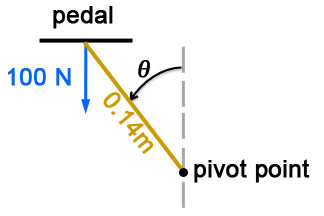
\includegraphics[width=0.4\textwidth]{ImgBicycle.jpg}
%      \caption{\small{The pedal arm (orange) rotates about the pivot point. The angle it makes with the vertical direction is $\theta$, measured counter-clockwise. A constant downward force of 100 N is applied to the pedal, which is attached to the other end of the pedal arm.}}
%  \end{center}
%\end{figure}
%\BEN
%  \item Determine the magnitude of the torque about the pivot point when $\theta$ is $30^{\circ}$ and when $\theta$ is $90^{\circ}$. Your answers should include the units of measurement. 
%  \item Determine the magnitude of the torque about the pivot point for any $\theta$. Your answer should be a function of $\theta$.  
%  \item What value(s) of $\theta$ minimize the produced torque? Briefly explain why. You should not need to compute any derivatives to answer this question. 
%\EEN
%Naturally, the torque vector can also be a function of time. In our bicycle example, the torque that is produced by the cyclist could change continuously as the pedal rotates about the pivot point. We will revisit the concept of torque as a vector function in a later assignment, after we have defined vector functions and their derivatives. 
%
%% -  -  -  -  -  -  -  -  -  -  -  -  -  -  -  -  -  -  -  -  -  -  -  -  -  -  -  -  -  -  

\EEN
\newpage % Page Break
% ~  ~  ~  ~  ~  ~  ~  ~  ~  ~  ~  ~  ~  ~  ~  ~  ~  ~  ~  ~  ~  ~  ~  ~
\subsection{Surfaces}
\rednote{We'll have 3 or 4 questions on this topic here.}
\newpage % Page Break
% ~  ~  ~  ~  ~  ~  ~  ~  ~  ~  ~  ~  ~  ~  ~  ~  ~  ~  ~  ~  ~  ~  ~  ~
\subsection{Curvilinear Coordinates}
\rednote{We'll have 3 or 4 questions on this topic here.}
\newpage % Page Break
% ~  ~  ~  ~  ~  ~  ~  ~  ~  ~  ~  ~  ~  ~  ~  ~  ~  ~  ~  ~  ~  ~  ~  ~
% VECTOR VALUED FUNCTIONS
\subsection{Vector-Valued Functions}

\purple{\From Section 1.8 of \VCT.}

\BEN

%% ~~~~~~~~~~~~~~~~~~~~~~~~~~~~~~~~~~~~~~~~~~~~~~~~~~~~~~~~~
%\item
%% QUESTION 
%For $A$ and \textbf{b} below, solve the linear system $A\mathbf{x} = \mathbf{b}$, if possible:
%\begin{align*}
% A = \BM
%  1 & 2 & 0 & 1 \\
%  3 & -1 & 1 & 2 \\
%  0 & 1 & 0 & 2 \\
%  4 & 0 & 3 & 1
% \EM, \ 
% \mathbf{b} = \BM 1 \\ 5 \\ 0 \\ 10 \EM.
%\end{align*}
% If it isn't possible to solve this system, explain why. 
%
%% ~~~~~~~~~~~~~~~~~~~~~~~~~~~~~~~~~~~~~~~~~~~~~~~~~~~~~~~~~
%\item
%% QUESTION 
%For the systems below,
%\begin{itemize}
%\item Compute the determinant of matrix $A$, if possible. If it is not possible to do so, explain why. 
%\item Solve the linear system $A\mathbf{x} = \mathbf{b}$, if possible. 
%\item State whether the system has no solution, infinitely many solutions, or a unique solution.
%\end{itemize}
%
%\begin{enumerate}
%\item \(
% A = \begin{bmatrix}
%  -3 &  1 & 2 &  4 \\
%   2 & -1 & 2 &  3 \\
%   1 &  0 & 4 & -2
% \end{bmatrix}, \ 
% \mathbf{b} = \begin{bmatrix} 1 \\ 1 \\ 1 \end{bmatrix}
%\)
%\item \( A = \begin{bmatrix}
% 1 & 2 & -1 \\
% 2 & 5 & 0 \\
% 4 & 9 & -2
%\end{bmatrix} , \ 
% \mathbf{b} =
%\begin{bmatrix} 1 \\ 2 \\ -1 \end{bmatrix} \)
%\end{enumerate}

% ~~~~~~~~~~~~~~~~~~~~~~~~~~~~~~~~~~~~~~~~~~~~~~~~~~~~~~~~~
\item 
% QUESTION
Find the values of $t$ and the points on the curve 
\begin{align*}
  \mathbf{r}(t) &= (1+t^2) \mathbf{i} + t\mathbf{j}, \quad t\in \R
\end{align*}
where
\begin{enumerate}
  \item $\mathbf{r}(t)$ and $\mathbf{r}'(t)$ are perpendicular,
  \item $\mathbf{r}(t)$ and $\mathbf{r}'(t)$ have the same direction, and
  \item $\mathbf{r}(t)$ and $\mathbf{r}'(t)$ have opposite directions.   
\end{enumerate}
%
%% ~~~~~~~~~~~~~~~~~~~~~~~~~~~~~~~~~~~~~~~~~~~~~~~~~~~~~~~~~
%\item 
%% QUESTION 4
%%GPS: MMCA2b
%
%Consider the system of simultaneous linear equations
%\begin{align*}
%  x + 2y -  z &= 2 \\
% 2x + ay - 2z &= b \\
% 3x + 2y      &= 1
%\end{align*}
%where $x, y, z$ are unknown.
%
%\begin{enumerate}
%\item Find all values of $a$ and $b$ such that the above system has
%\begin{enumerate}
%\item \label{q:one_solution} exactly one solution;
%\item no solutions;
%\item \label{q:many_solutions} infinitely many solutions.
%\end{enumerate}
%\item For those values of $a$ and $b$ from~\ref{q:one_solution}, what is the
%unique solution?
%\item For those values of $a$ and $b$ from~\ref{q:many_solutions},
% parameterize the set of all solutions.
%\end{enumerate}
%
%% ~~~~~~~~~~~~~~~~~~~~~~~~~~~~~~~~~~~~~~~~~~~~~~~~~~~~~~~~~
%
\item \textbf{Application to Mechanics}\\
%For $t\in\R$, the real valued functions
%\begin{align*}
%y(t)=2+5t, \quad y(t) = \sin(4t) , \quad y(t)=e^{6t}
%\end{align*}
%are referred to as \textbf{scalar functions}, because in each case, they assign a real number $y$, to another real number $t$. However, functions such as
%\begin{align*}
%\mathbf{v}(t)=\mathbf{r}_0+t\mathbf{r}, \quad \mathbf{v}(t) = \sin(4t)\mathbf{a} , \quad \mathbf{v}(t)=e^{6t}\mathbf{b}
%\end{align*}
%assign a vector to real numbers, and are referred to as \textbf{vector functions}. They could be used, for example if the position of a particle is specified by the vector $\mathbf{r}\in \R^3$, and that the particle is moving, so that \textbf{r} is a function of time: \textbf{r}=\textbf{r}$(t)$. 
%
%Many of the properties of vector functions are intuitive. For example, the derivative of a vector function, defined as
%\begin{align*}
%\lim_{h\rightarrow0} \frac{\mathbf{r}(t+h) - \mathbf{r}(t)}{h}
%\end{align*}
%describes the rate of change of $\mathbf{r}$ at $t$ (provided that the limit exists). If the vector \textbf{r} represents the position of a particle at time $t$, then, naturally, $\mathbf{r}'(t)$ represents its velocity at time $t$, and $\mathbf{r}''(t)$ represents its acceleration at time $t$. Moreover, we can compute the derivative of a vector by simply taking the derivative of each of its components separately. For example, if $\mathbf{v}(t) = 5t \mathbf{i} + \cos(t)\mathbf{j} - \mathbf{k}$, then $\mathbf{v}'(t) = 5 \mathbf{i} - \sin(t)\mathbf{j} - 0 \mathbf{k}$, or 
%\begin{align*}
% \frac{d \mathbf{v}(t)}{dt} = \mathbf{v}'(t) &= \BM 5 \\ -\sin(t) \\ 0 \EM.
%\end{align*}
%Differentiation rules for scalar multiplication, cross and dot products can also be derived and resemble the product rule for scalar functions:
%\begin{align*}
%\frac{d}{dt} \big( C \mathbf{u}(t)\big) &=C \frac{d \mathbf{u}(t) }{dt}  , \quad C \text{ is a constant} \\
%\frac{d}{dt} \big( \mathbf{v}(t) \cdot \mathbf{u}(t)\big) &= \mathbf{v}(t) \cdot \frac{d \mathbf{u}(t) }{dt}  +  \frac{d \mathbf{v}(t)}{dt}  \cdot  \mathbf{u}(t) \\
%\frac{d}{dt} \big( \mathbf{v}(t) \times \mathbf{u}(t)\big) &= \mathbf{v}(t) \times \frac{d \mathbf{u}(t) }{dt}  +  \frac{d \mathbf{v}(t)}{dt}  \times  \mathbf{u}(t) 
%\end{align*}
%Other differentiation formulas that you may need throughout this course are provided in your textbook. \\\\
%\noindent\textbf{Questions}
Recall from a previous assignment that we defined torque as $\boldsymbol\tau = \mathbf{r} \times \MB{F}$. Now that we have introduced the concepts of vector-valued functions and their derivatives, let's consider the more general case when $\boldsymbol\tau$, $\MB{r}$, and $\MB{F}$ are all functions of time:
\begin{align*}
  \boldsymbol\tau(t) &= \mathbf{r}(t) \times \MB{F}(t).
\end{align*}
Moreover, using the relation $\MB{F}(t)=m\MB{a}(t)$ (Newton's second law), we can write our definition of torque as
\begin{align*}
  \boldsymbol\tau(t) &= \mathbf{r}(t) \times \MB{F}(t) \\
  &= \mathbf{r}(t) \times \big(m\MB{a}(t)\big) \\
  &= m\big( \mathbf{r}(t) \times \mathbf{r}''(t)\big).
\end{align*}
These alternate forms for the torque vector may be helpful in solving the following problems.
\begin{enumerate}
\item If the position of a particle with mass $m$ is given by the position vector $\mathbf{r}(t)$, then its angular momentum is a vector defined as $\mathbf{L}(t) = m\mathbf{r}(t)\times \mathbf{r}'(t)$. Show that $\mathbf{L}'(t) = \boldsymbol\tau(t)$.
\item Show that if the torque is a zero vector for all $t$, then the angular momentum of the particle is constant for all $t$. This is what is known as the \Emph{law of conservation of angular momentum}.
\end{enumerate}
%% ~~~~~~~~~~~~~~~~~~~~~~~~~~~~~~~~~~~~~~~~~~~~~~~~~~~~~~~~~
%% POLYNOMIAL INTERPOLATION 
%\item \textbf{Application to Polynomial Interpolation}
%
%In many areas of engineering, experimental data is collected that must be analyzed to extract parameters that tell us something about a physical process. Suppose we have measured a set of experimental data that are represented in the $xy$-plane. An \Emph{interpreting polynomial} for the measured data is a polynomial that passes through every measured point. We can use this polynomial, for example, to estimate values between the measured data points. \\
%
%Suppose for example that we have measured the data points (0,-6), (1,-2), (2,4), (3,10). To find an interpreting polynomial of order 2 for these data, we would try to find a polynomial of the form $p(x) = a_0+a_1x+a_2x^2$ that passes through all four measured points. In other words, we need to find the unknown constants $a_0, a_1, a_2$ that satisfy the equations
%\begin{align*}
%p(0) = a_0+a_1(0)+a_2(0)^2 &= -6 \\
%p(1) = a_0+a_1(1)+a_2(1)^2 &= -2 \\
%p(2) = a_0+a_1(2)+a_2(2)^2 &= 4  \\
%p(3) = a_0+a_1(3)+a_2(3)^2 &= 10 
%\end{align*}
%The above system has four equations and four unknowns. Upon solving this system, you should be able to determine that $a_0 = -6, a_1 = 4, a_2=0$.\\
%
%\textbf{Wind Tunnel Experiment}\\
%In a fictitious wind tunnel experiment, the following measurements were made. 
%\begin{center}
%  \begin{tabular}{ c c }
%    Velocity (m/s) & Force (N)  \\ \hline
%     0  & 0 \\
%    1 & 5.5 \\
%    2 & 20 \\
%    3 & 46.5 \\
%    4 & 88
%  \end{tabular}
%\end{center}
%
%The data represent the measured force due to air resistance, on an object suspended in the tunnel, measured at different air speed velocities.
%\begin{enumerate}
%\item Using the data above, derive a $5\times4$ system of equations, that when solved, find an interpreting polynomial of the form $p(x) = a_0+a_1x+a_2x^2+a_3x^3$. Write the system in the form $A\mathbf{x}=\mathbf{b}$.
%\item Solve your system to obtain $p(x) = a_0+a_1x+a_2x^2+a_3x^3$.
%\item As mentioned above, engineers sometimes use interpreting polynomials to estimate values in between measured data points. Using your polynomial, estimate the value of the force when the velocity is 1.5 m/s. 
%\item In practice, it can be difficult to determine what order of polynomial to use. Sometimes, polynomials of different orders must be used to decide which polynomial yields the most useful results. For the above data, explain what what would happen if we used a polynomial less than 3. It may help to see what happens if we use a 1$^{st}$ order polynomial. 
%\end{enumerate}
%\begin{figure}[h]
%  \vspace{-5pt}
%  \begin{center}
%    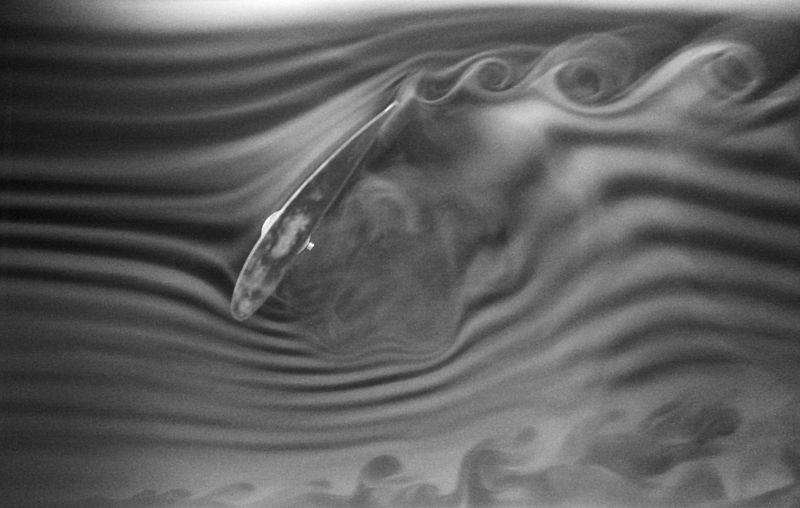
\includegraphics[width=0.6\textwidth]{ImgWindTunnel.jpg}
%  \end{center}
%  \vspace{-20pt}
%  \caption{\small{An airfoil in a fog wind tunnel (image from Wikimedia Commons, Smart Blade GmbH).}}
%\end{figure}
% ~~~~~~~~~~~~~~~~~~~~~~~~~~~~~~~~~~~~~~~~~~~~~~~~~~~~~~~~~
% PARTICLE MOTION
\item 
\textbf{Integration with Vector-Valued Functions}\\
If the position of a particle is given by the vector function $\MB{r}(t) \in \R^3$, then we know that we can determine its velocity, $\MB{v}(t)= \MB{r}'(t)$, by differentiating each of its components. That is, if 
\begin{align*}
  \MB{r}(t) = \BM r_1(t) \\ r_2(t) \\ r_3(t) \EM,
\end{align*}
then
\begin{align*}
  \MB{v}(t)= \MB{r}'(t) = \BM \frac{d}{dt} r_1(t) \\ \frac{d}{dt} r_2(t) \\ \frac{d}{dt} r_3(t) \EM = \BM v_1(t) \\ v_2(t) \\ v_3(t) \EM,
\end{align*}
provided that the derivatives of the components of $\MB{r}$ exist at $t$. It follows from the Fundamental Theorem of Calculus that if we were instead given the velocity of the particle, we could compute its position by integrating each of the components with respect to $t$. We would of course introduce constants of integration. That is, given
\begin{align*}
  \MB{v}(t) = \BM v_1(t) \\ v_2(t) \\ v_3(t) \EM, 
\end{align*}
we could obtain $\MB{r}$ by integrating each of the components of $\MB{v}(t)$
\begin{align*}
  \MB{r}(t) = \BM \int v_1(t) dt \\ \int v_2(t) dt \\ \int v_3(t) dt \EM = \BM r_1(t) + c_1 \\ r_2(t) +c_2 \\ r_3(t) +c_3 \EM,
\end{align*}
where $c_1,c_2,c_3$ are constants. 

Suppose that a particle with mass $m$ is subjected to a force, $\MB{F}(t) = m\pi^2\big(\cos(\pi t)\MB{j}+\sin(\pi t)\MB{k}\big)$, where $t \ge 0$. Suppose also that when $t=0$, 
\begin{align*}
  \MB{r}(0) &= \BM -1 \\ 0 \\ 0 \EM , \quad
  \MB{r}'(0) = \BM +1 \\ 0 \\ 0 \EM.
\end{align*}
\BEN
\item Using the relation $\MB{F} = m\MB{a}$, find the velocity of the particle at time $t$. \textit{Hint: you will need to apply the velocity at time t=0}.
\item Find the position of the particle at time $t=1$.
\item Plot the position of the particle at times $t=0$ and $t=1$ on the same graph in $\R^3$.
\EEN
% ~~~~~~~~~~~~~~~~~~~~~~~~~~~~~~~~~~~~~~~~~~~~~~~~~~~~~~~~~
\EEN % END OF QUESTIONS


\newpage % Page Break
% ~  ~  ~  ~  ~  ~  ~  ~  ~  ~  ~  ~  ~  ~  ~  ~  ~  ~  ~  ~  ~  ~  ~  ~
% LINEAR SYSTEMS
\subsection{Linear Systems}

\FromC{\From Section 8.1 of \CAT.}


\BEN

% ~~~~~~~~~~~~~~~~~~~~~~~~~~~~~~~~~~~~~~~~~~~~~~~~~~~~~~~~~
\item
% QUESTION 
For $A$ and \textbf{b} below, solve the linear system $A\mathbf{x} = \mathbf{b}$, if possible:
\begin{align*}
 A = \BM
  1 & 2 & 0 & 1 \\
  3 & -1 & 1 & 2 \\
  0 & 1 & 0 & 2 \\
  4 & 0 & 3 & 1
 \EM, \ 
 \mathbf{b} = \BM 1 \\ 5 \\ 0 \\ 10 \EM.
\end{align*}
 If it isn't possible to solve this system, explain why. 

% ~~~~~~~~~~~~~~~~~~~~~~~~~~~~~~~~~~~~~~~~~~~~~~~~~~~~~~~~~
\item
% QUESTION 
For the systems below,
\begin{itemize}
\item Compute the determinant of matrix $A$, if possible. If it is not possible to do so, explain why. 
\item Solve the linear system $A\mathbf{x} = \mathbf{b}$, if possible. 
\item State whether the system has no solution, infinitely many solutions, or a unique solution.
\end{itemize}

\begin{enumerate}
\item \(
 A = \begin{bmatrix}
  -3 &  1 & 2 &  4 \\
   2 & -1 & 2 &  3 \\
   1 &  0 & 4 & -2
 \end{bmatrix}, \ 
 \mathbf{b} = \begin{bmatrix} 1 \\ 1 \\ 1 \end{bmatrix}
\)
\item \( A = \begin{bmatrix}
 1 & 2 & -1 \\
 2 & 5 & 0 \\
 4 & 9 & -2
\end{bmatrix} , \ 
 \mathbf{b} =
\begin{bmatrix} 1 \\ 2 \\ -1 \end{bmatrix} \)
\end{enumerate}

%% ~~~~~~~~~~~~~~~~~~~~~~~~~~~~~~~~~~~~~~~~~~~~~~~~~~~~~~~~~
%\item 
%% QUESTION
%Find the values of $t$ and the points on the curve 
%\begin{align*}
%  \mathbf{r}(t) &= (1+t^2) \mathbf{i} + t\mathbf{j}, \quad t\in \R
%\end{align*}
%where
%\begin{enumerate}
%  \item $\mathbf{r}(t)$ and $\mathbf{r}'(t)$ are perpendicular,
%  \item $\mathbf{r}(t)$ and $\mathbf{r}'(t)$ have the same direction, and
%  \item $\mathbf{r}(t)$ and $\mathbf{r}'(t)$ have opposite directions.   
%\end{enumerate}

% ~~~~~~~~~~~~~~~~~~~~~~~~~~~~~~~~~~~~~~~~~~~~~~~~~~~~~~~~~
\item 
% QUESTION 4
%GPS: MMCA2b

Consider the system of simultaneous linear equations
\begin{align*}
  x + 2y -  z &= 2 \\
 2x + ay - 2z &= b \\
 3x + 2y      &= 1
\end{align*}
where $x, y, z$ are unknown.

\begin{enumerate}
\item Find all values of $a$ and $b$ such that the above system has
\begin{enumerate}
\item \label{q:one_solution} exactly one solution;
\item no solutions;
\item \label{q:many_solutions} infinitely many solutions.
\end{enumerate}
\item For those values of $a$ and $b$ from~\ref{q:one_solution}, what is the
unique solution?
\item For those values of $a$ and $b$ from~\ref{q:many_solutions},
 parameterize the set of all solutions.
\end{enumerate}

% ~~~~~~~~~~~~~~~~~~~~~~~~~~~~~~~~~~~~~~~~~~~~~~~~~~~~~~~~~

%\item \textbf{Application to Mechanics}\\
%For $t\in\R$, the real valued functions
%\begin{align*}
%y(t)=2+5t, \quad y(t) = \sin(4t) , \quad y(t)=e^{6t}
%\end{align*}
%are referred to as \textbf{scalar functions}, because in each case, they assign a real number $y$, to another real number $t$. However, functions such as
%\begin{align*}
%\mathbf{v}(t)=\mathbf{r}_0+t\mathbf{r}, \quad \mathbf{v}(t) = \sin(4t)\mathbf{a} , \quad \mathbf{v}(t)=e^{6t}\mathbf{b}
%\end{align*}
%assign a vector to real numbers, and are referred to as \textbf{vector functions}. They could be used, for example if the position of a particle is specified by the vector $\mathbf{r}\in \R^3$, and that the particle is moving, so that \textbf{r} is a function of time: \textbf{r}=\textbf{r}$(t)$. 
%
%Many of the properties of vector functions are intuitive. For example, the derivative of a vector function, defined as
%\begin{align*}
%\lim_{h\rightarrow0} \frac{\mathbf{r}(t+h) - \mathbf{r}(t)}{h}
%\end{align*}
%describes the rate of change of $\mathbf{r}$ at $t$ (provided that the limit exists). If the vector \textbf{r} represents the position of a particle at time $t$, then, naturally, $\mathbf{r}'(t)$ represents its velocity at time $t$, and $\mathbf{r}''(t)$ represents its acceleration at time $t$. Moreover, we can compute the derivative of a vector by simply taking the derivative of each of its components separately. For example, if $\mathbf{v}(t) = 5t \mathbf{i} + \cos(t)\mathbf{j} - \mathbf{k}$, then $\mathbf{v}'(t) = 5 \mathbf{i} - \sin(t)\mathbf{j} - 0 \mathbf{k}$, or 
%\begin{align*}
% \frac{d \mathbf{v}(t)}{dt} = \mathbf{v}'(t) &= \BM 5 \\ -\sin(t) \\ 0 \EM.
%\end{align*}
%Differentiation rules for scalar multiplication, cross and dot products can also be derived and resemble the product rule for scalar functions:
%\begin{align*}
%\frac{d}{dt} \big( C \mathbf{u}(t)\big) &=C \frac{d \mathbf{u}(t) }{dt}  , \quad C \text{ is a constant} \\
%\frac{d}{dt} \big( \mathbf{v}(t) \cdot \mathbf{u}(t)\big) &= \mathbf{v}(t) \cdot \frac{d \mathbf{u}(t) }{dt}  +  \frac{d \mathbf{v}(t)}{dt}  \cdot  \mathbf{u}(t) \\
%\frac{d}{dt} \big( \mathbf{v}(t) \times \mathbf{u}(t)\big) &= \mathbf{v}(t) \times \frac{d \mathbf{u}(t) }{dt}  +  \frac{d \mathbf{v}(t)}{dt}  \times  \mathbf{u}(t) 
%\end{align*}
%Other differentiation formulas that you may need throughout this course are provided in your textbook. \\\\
%%\noindent\textbf{Questions}
%Recall from a previous assignment that we defined torque as $\boldsymbol\tau = \mathbf{r} \times \MB{F}$. Now that we have introduced the concepts of vector-valued functions and their derivatives, let's consider the more general case when $\boldsymbol\tau$, $\MB{r}$, and $\MB{F}$ are all functions of time:
%\begin{align*}
%  \boldsymbol\tau(t) &= \mathbf{r}(t) \times \MB{F}(t).
%\end{align*}
%Moreover, using the relation $\MB{F}(t)=m\MB{a}(t)$ (Newton's second law), we can write our definition of torque as
%\begin{align*}
%  \boldsymbol\tau(t) &= \mathbf{r}(t) \times \MB{F}(t) \\
%  &= \mathbf{r}(t) \times \big(m\MB{a}(t)\big) \\
%  &= m\big( \mathbf{r}(t) \times \mathbf{r}''(t)\big).
%\end{align*}
%These alternate forms for the torque vector may be helpful in solving the following problems.
%\begin{enumerate}
%\item If the position of a particle with mass $m$ is given by the position vector $\mathbf{r}(t)$, then its angular momentum is a vector defined as $\mathbf{L}(t) = m\mathbf{r}(t)\times \mathbf{r}'(t)$. Show that $\mathbf{L}'(t) = \boldsymbol\tau(t)$.
%\item Show that if the torque is a zero vector for all $t$, then the angular momentum of the particle is constant for all $t$. This is what is known as the \Emph{law of conservation of angular momentum}.
%\end{enumerate}
% ~~~~~~~~~~~~~~~~~~~~~~~~~~~~~~~~~~~~~~~~~~~~~~~~~~~~~~~~~
% POLYNOMIAL INTERPOLATION 
\item \textbf{Application to Polynomial Interpolation}

In many areas of engineering, experimental data is collected that must be analyzed to extract parameters that tell us something about a physical process. Suppose we have measured a set of experimental data that are represented in the $xy$-plane. An \Emph{interpreting polynomial} for the measured data is a polynomial that passes through every measured point. We can use this polynomial, for example, to estimate values between the measured data points. \\

Suppose for example that we have measured the data points (0,-6), (1,-2), (2,4), (3,10). To find an interpreting polynomial of order 2 for these data, we would try to find a polynomial of the form $p(x) = a_0+a_1x+a_2x^2$ that passes through all four measured points. In other words, we need to find the unknown constants $a_0, a_1, a_2$ that satisfy the equations
\begin{align*}
p(0) = a_0+a_1(0)+a_2(0)^2 &= -6 \\
p(1) = a_0+a_1(1)+a_2(1)^2 &= -2 \\
p(2) = a_0+a_1(2)+a_2(2)^2 &= 4  \\
p(3) = a_0+a_1(3)+a_2(3)^2 &= 10 
\end{align*}
The above system has four equations and four unknowns. Upon solving this system, you should be able to determine that $a_0 = -6, a_1 = 4, a_2=0$.\\

\textbf{Wind Tunnel Experiment}\\
In a fictitious wind tunnel experiment\footnote{The wind tunnel problem was based on a similar exercise in Linear Algebra and Its Applications, 4th Edition, by David C. Lay, Addison-Wesley, 2012.}, the following measurements were made. 
\begin{center}
  \begin{tabular}{ c c }
    Velocity (m/s) & Force (N)  \\ \hline
     0  & 0 \\
    1 & 5.5 \\
    2 & 20 \\
    3 & 46.5 \\
    4 & 88
  \end{tabular}
\end{center}

The data represent the measured force due to air resistance, on an object suspended in the tunnel, measured at different air speed velocities.
\begin{enumerate}
\item Using the data above, derive a $5\times4$ system of equations, that when solved, find an interpreting polynomial of the form $p(x) = a_0+a_1x+a_2x^2+a_3x^3$. Write the system in the form $A\mathbf{x}=\mathbf{b}$.
\item Solve your system to obtain $p(x) = a_0+a_1x+a_2x^2+a_3x^3$.
\item As mentioned above, engineers sometimes use interpreting polynomials to estimate values in between measured data points. Using your polynomial, estimate the value of the force when the velocity is 1.5 m/s. 
\item In practice, it can be difficult to determine what order of polynomial to use. Sometimes, polynomials of different orders must be used to decide which polynomial yields the most useful results. For the above data, explain what what would happen if we used a polynomial less than 3. It may help to see what happens if we use a 1$^{st}$ order polynomial. 
\end{enumerate}
\begin{figure}[h]
  \vspace{-5pt}
  \begin{center}
    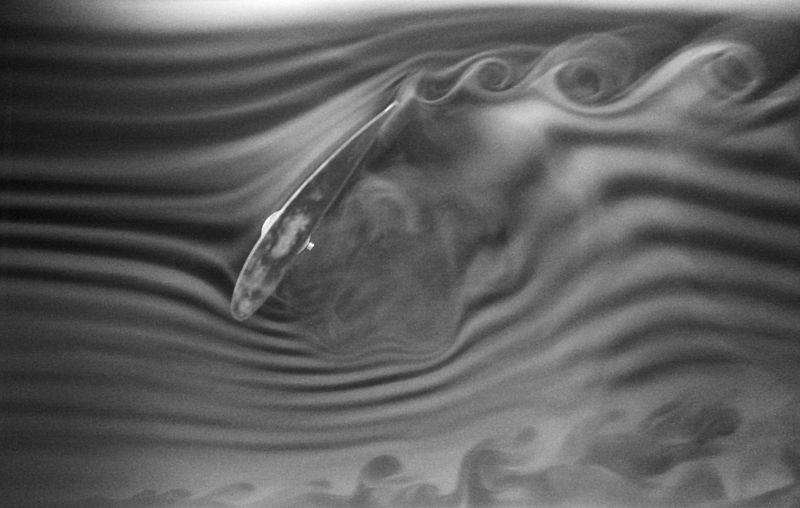
\includegraphics[width=0.6\textwidth]{ImgWindTunnel.jpg}
  \end{center}
  \vspace{-20pt}
  \caption{\small{An airfoil in a fog wind tunnel (image from Wikimedia Commons, Smart Blade GmbH).}}
\end{figure}

\EEN % END OF QUESTIONS




\newpage % Page Break
% ~  ~  ~  ~  ~  ~  ~  ~  ~  ~  ~  ~  ~  ~  ~  ~  ~  ~  ~  ~  ~  ~  ~  ~
%\section{Partial Derivatives}
\section{Partial Derivatives}
\setcounter{subsection}{-1}
\subsection{Partial Derivatives}
\FromC{\From sections 2.2 through 2.4 of \VCT.}

\BEN

% ~~~~~~~~~~~~~~~~~~~~~~~~~~~~~~~~~~~~~~~~~~~~~~~~~~~~~~~~~
\item

Compute all first and second partial derivatives and the gradient
for each of the following functions.
\begin{enumerate}
 \item $f(x,y) = xy\sin(\frac{x}{y})$
 \item $g(x,y) = \dfrac{x+y}{e^{xy}}$
\end{enumerate}

% ~~~~~~~~~~~~~~~~~~~~~~~~~~~~~~~~~~~~~~~~~~~~~~~~~~~~~~~~~
\item

Compute the gradient of the function $z = h(x, y)$ defined implicitly by the
equation $xy = z^{x+y}$.

% ~~~~~~~~~~~~~~~~~~~~~~~~~~~~~~~~~~~~~~~~~~~~~~~~~~~~~~~~~
\item

Find the equations of the planes tangent to the following surfaces
at the specified points.
\begin{enumerate}
 \item $f(x,y) = \frac{x^2}{9} - y^2$ at the point $(2, \frac{1}{3})$.
 \item $x^2 + x + y - z^2 = 7$ at the point $(2, 5, 2)$.
\end{enumerate}

% ~~~~~~~~~~~~~~~~~~~~~~~~~~~~~~~~~~~~~~~~~~~~~~~~~~~~~~~~~
\item

Let $f(x,y) = e^{-(x^2+x+1+y^2-2y)}$.
\begin{enumerate}
 \item In which direction does $f$ increase fastest from the point
  (1,1)?
 \item Compute the rate of change of $f$ in the direction of the
  point $(5,4)$ from the point $(2,1)$.
\end{enumerate}

% ~~~~~~~~~~~~~~~~~~~~~~~~~~~~~~~~~~~~~~~~~~~~~~~~~~~~~~~~~
\item

Find the Jacobian matrix for the function
$f(x,y) = \begin{bmatrix} \sin(x+y) \\ \ln(xy) \end{bmatrix}$.

% ~~~~~~~~~~~~~~~~~~~~~~~~~~~~~~~~~~~~~~~~~~~~~~~~~~~~~~~~~
\item
\Emph{Application: The Heat Equation}

A \emph{partial differential equation} is an equation that involves
the partial derivatives of a function.  For example,
$(\frac{\partial f}{\partial x})^2 - \frac{\partial^2 f}{\partial x
\partial y} = 0$ is a partial differential equation that relates
the first- and second-order partial derivatives of an unknown function
$f$.

A function $f$ is said to \emph{satisfy} a partial differential
equation when the equation holds upon substitution of the function's
partial derivatives.  For example, the function $f(x, y) = y$
satisfies the above partial differential equation since
$(\frac{\partial}{\partial x}(y))^2 = 0$ and $\frac{\partial^2}{\partial x \partial y}(y) = \frac{\partial}{\partial x}(1) = 0$.

The one-dimensional heat equation is a partial differential equation
which relates physical properties of a material to the function that
specifies the exact temperature at any point along a fixed-length rod
of that material.  Under a few assumptions, it can be stated in the
following form:
\begin{equation}
\frac{\partial u}{\partial t} = \frac{K_0}{c\rho} \frac{\partial^2 u}{\partial x^2} \label{eqn:heat}
\end{equation}
where $u = u(x,t)$, $x$ is the position along the rod, $t$ is the point in time,
$K_0$ is the thermal conductivity of the material, $c$ is its specific heat,
and $\rho$ is its mass density.

Show that $u(x,t) = e^{-tK_0/(c\rho)}\sin(x)$ is a solution to (\ref{eqn:heat}).

\EEN

% ----------------------------------------------------------------------------
\newpage
\subsection{Optimization}
\FromC{\From sections 2.5, 2.7 and parts of 4.6 of \VCT.}

\BEN

% ~~~~~~~~~~~~~~~~~~~~~~~~~~~~~~~~~~~~~~~~~~~~~~~~~~~~~~~~~
\item

Use the second derivative test to classify the local extrema of the
following functions:
\begin{enumerate}
 \item $f(x,y) = x^2 + 2x - xy + y^2$
 \item $h(x,y) = \sin(xy)$
\end{enumerate}

% ~~~~~~~~~~~~~~~~~~~~~~~~~~~~~~~~~~~~~~~~~~~~~~~~~~~~~~~~~
\item

Find the extreme values of
\begin{enumerate}
 \item the function
  $f(x,y) = e^{-(x^2+y^2)}$
  along the curve $x = y^2$
 \item the function
  $g(x,y) = e^{x-y^2}$ along the boundary of the ellipse
  $\frac{x^2}{4}+y+y^2=1$
\end{enumerate}

% ~~~~~~~~~~~~~~~~~~~~~~~~~~~~~~~~~~~~~~~~~~~~~~~~~~~~~~~~~
\item

Consider the function $f(x,y,z) = \begin{bmatrix}
                                   x^2 + y^2 \\
                                   y^2 + z^2 \\
                                   z^2 + x^2
                                  \end{bmatrix}$.
Find its divergence $\nabla \cdot f$ and curl $\nabla \times f$.

% ~~~~~~~~~~~~~~~~~~~~~~~~~~~~~~~~~~~~~~~~~~~~~~~~~~~~~~~~~
\item

Find the point on the sphere $x^2 + y^2 + z^2 = 1$ that is closest
to the plane $x + 2y + 2z = 5$. (Hint: using some geometric intuition
is is possible to complete this problem without using the method of
Lagrange multipliers.)

% ~~~~~~~~~~~~~~~~~~~~~~~~~~~~~~~~~~~~~~~~~~~~~~~~~~~~~~~~~
\item
\Emph{Application: Cost Optimization}

Suppose you are given a budget of \$500 to build a large glass
triangular prism.  Each rectangular side must have equal dimensions
and the two triangular sides must also have equal dimensions.  You
can purchase glass for the rectangular sides at a cost of $\$8/ft^2$
and for the triangular sides at a cost of $\$10/ft^2$.

What are the dimensions of the prism of largest volume that you can build?

% ~~~~~~~~~~~~~~~~~~~~~~~~~~~~~~~~~~~~~~~~~~~~~~~~~~~~~~~~~
\item
\Emph{Application: Heat Optimization}

Suppose that the temperature in a space is given by the function
$T(x,y,z) = 200xyz^2$.  Find the hottest point on the unit sphere.

(This question taken from section 4.5 of {\it Vector Calculus} by Susan Colley)

\EEN

\newpage % Page Break
% ~  ~  ~  ~  ~  ~  ~  ~  ~  ~  ~  ~  ~  ~  ~  ~  ~  ~  ~  ~  ~  ~  ~  ~
\section{Multiple Integrals}
%\setcounter{subsection}{-1}

% s~s~s~s~s~s~s~s~s~s~s~s~s~s~s~s~s~s~s~s~s~s~s~s~s~s~s~s~s~s~s~s~s~s~s~s~s~s~s~s~s~s~s~s
% s~s~s~s~s~s~s~s~s~s~s~s~s~s~s~s~s~s~s~s~s~s~s~s~s~s~s~s~s~s~s~s~s~s~s~s~s~s~s~s~s~s~s~s
\subsection{Wolfram Alpha Syntax (optional)}
You may want to use Wolfram Alpha (wolframalpha.com) to check your answers. If you're not sure what syntax to use to compute double integrals with Wolfram Alpha, let's suppose that we want to determine the value of
\begin{align*} 
   \mathop{\int_{-2}^{-1} \!  \int_0^{x-1}}( x^{2C} +y)  dy  dx
\end{align*}
where $C$ is a constant. The syntax we could use to compute this particular integral is
\begin{quote}
  \begin{verbatim}
    integrate x^{2C}+y dydx, x from -2 to -1 and y from 0 to (x-1)
  \end{verbatim}
\end{quote}
% END OF SUBSECTION
% s~s~s~s~s~s~s~s~s~s~s~s~s~s~s~s~s~s~s~s~s~s~s~s~s~s~s~s~s~s~s~s~s~s~s~s~s~s~s~s~s~s~s~s
% s~s~s~s~s~s~s~s~s~s~s~s~s~s~s~s~s~s~s~s~s~s~s~s~s~s~s~s~s~s~s~s~s~s~s~s~s~s~s~s~s~s~s~s
\subsection{Double Integrals}
\purple{\From Section 3.1 of \VCT.}

\BEN
% ~~~~~~~~~~~~~~~~~~~~~~~~~~~~~~~~~~~~~~~~~~~~~~~~~~~~~~~~~~~~~~~~~~~~~~~~~~~~~~~~~
\item % VOLUME OF SIMPLE SOLID 
Consider the solid that lies under the plane $z = -x-2y+2$ and above the rectangle \\$\{(x,y) \ | \ -2\le x\le 0, 0\le y \le1 \}$.
\BEN
\item Sketch the solid in $\R^3$. \textit{Hint: start by plotting the points that are located on the given plane and above the corners of the rectangle. Then connect the points with solid lines.}
\item Find the volume of the solid.
\EEN
% ~~~~~~~~~~~~~~~~~~~~~~~~~~~~~~~~~~~~~~~~~~~~~~~~~~~~~~~~~~~~~~~~~~~~~~~~~~~~~~~~~
\item % FLUID MECHANICS
\textbf{Application to Fluid Mechanics} \\
In a two-dimensional, steady-state, incompressible fluid flow, the velocity \textbf{v} of the flow can be expressed as $\MB{v} = u(x,y)\MB{i} + v(x,y)\MB{j}$. The functions $u(x,y)$ and $v(x,y)$ must satisfy 
\begin{align*}
  \nabla\cdot\MB{v} = 0.
\end{align*}
\BEN
\item If $u(x,y) = x^2 + y^2$, find the most general form of $v(x,y)$. 
\item If $v(x,y) = \cos(x)$, find the most general form of $u(x,y)$.
\EEN
\textit{Hint: you are asked to find the most \Emph{general} form of functions u and v}.

\EEN % END OF SUBSECTION
% s~s~s~s~s~s~s~s~s~s~s~s~s~s~s~s~s~s~s~s~s~s~s~s~s~s~s~s~s~s~s~s~s~s~s~s~s~s~s~s~s~s~s~s
% s~s~s~s~s~s~s~s~s~s~s~s~s~s~s~s~s~s~s~s~s~s~s~s~s~s~s~s~s~s~s~s~s~s~s~s~s~s~s~s~s~s~s~s
\subsection{Double Integrals Over a General Region}
\purple{\From Section 3.2 of \VCT.}

\BEN
% ~~~~~~~~~~~~~~~~~~~~~~~~~~~~~~~~~~~~~~~~~~~~~~~~~~~~~~~~~~~~~~~~~~~~~~~~~~~~~~~~~
\item % TETRAHEDRON
\Emph{Volume of a Tetrahedron} \\
A \Emph{tetrahedron} is a three dimensional object with four, triangular, flat sides. Because each of its four sides are flat, a tetrahedron can be defined as the region enclosed by four planes. Below is a sketch of two tetrahedrons. Note that each tetrahedron has four vertices, six edges, and that the lengths of its edges do not have to be equal.
\begin{figure}[h]
  \vspace{-1pt}
  \begin{center}
    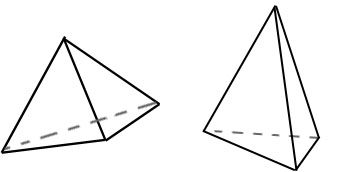
\includegraphics[width=0.35\textwidth]{ImgTetrahedrons.jpg}
  \end{center}
\end{figure}\\
Consider the tetrahedron that is bounded by the three coordinate planes in $\R^3$, and by the plane $z = 1 - x - \frac{y}{2}$.
\BEN
\item Sketch the tetrahedron in $\R^3$ and label the points that represent its four vertices. 
\item Set up, but do not evaluate, a double integral that represents the volume of the tetrahedron. Integrate with respect to $x$ first. 
\item Set up, but do not evaluate, a double integral that represents the volume of the tetrahedron. Integrate with respect to $y$ first. 
\EEN
Note that
\begin{itemize}
\item Examples 3.4 and 3.5 from \VCT \ are similar to this problem. 
\item We could also calculate the volume of the solid by using a \Emph{triple} integral. 
\item Although not required, the double integrals are straightforward to compute. You may want to check your answers by evaluating the integrals and seeing if you would get the same result in parts (b) and (c). 
\end{itemize}
% ~~~~~~~~~~~~~~~~~~~~~~~~~~~~~~~~~~~~~~~~~~~~~~~~~~~~~~~~~~~~~~~~~~~~~~~~~~~~~~~~~
\item  % DESCRIBE WHY A PARTICULAR DOUBLE INTEGRAL GIVES AREA
\Emph{Area of a General Region}
\BEN
\item Question 11 from Section 3.2 of \VCT. \textit{Hint: Figure 3.2.5 is also helpful.}
\item Use the result from part (a) to compute the area of the region bounded by the curves $y = x^2$ and $x=y^2$.
\EEN

% ~~~~~~~~~~~~~~~~~~~~~~~~~~~~~~~~~~~~~~~~~~~~~~~~~~~~~~~~~~~~~~~~~~~~~~~~~~~~~~~~~
\item % UPPER AND LOWER BOUNDS ARE FUNCTIONS
Find the volume of the solid enclosed by $z = x^2 + y^2$, $y = x^2$ and $x=y^2$.
% ~~~~~~~~~~~~~~~~~~~~~~~~~~~~~~~~~~~~~~~~~~~~~~~~~~~~~~~~~~~~~~~~~~~~~~~~~~~~~~~~~
\item % CHANGING ORDER OF INTEGRATION
Consider the integral
\begin{align*}
  \iint\limits_R x\sin(y) dA
\end{align*}
 where $R$ is the region bounded by $y=0$, $y=x^2$, and $x=2$.
\BEN
\item Evaluate the double integral by first integrating with respect to $x$. 
\item Evaluate the double integral by first integrating with respect to $y$. 
\EEN
Note that your answers for both parts should be the same, and that you may need to use various techniques of integration to complete this problem, including integration by parts and a variable substitution. 
% ~~~~~~~~~~~~~~~~~~~~~~~~~~~~~~~~~~~~~~~~~~~~~~~~~~~~~~~~~~~~~~~~~~~~~~~~~~~~~~~~~
\item % CHANGING ORDER OF INTEGRATION, GENERAL F(X,Y)
Consider the double integral
\begin{align*}
  \mathop{\int_{0}^{1+e} \! \int_0^{\ln(x-1)}} f(x,y) dydx .
\end{align*}
Sketch the region in $\R^2$ over which $f(x,y)$ is integrated, and change the order of integration.  
% ~~~~~~~~~~~~~~~~~~~~~~~~~~~~~~~~~~~~~~~~~~~~~~~~~~~~~~~~~~~~~~~~~~~~~~~~~~~~~~~~~
\item % BOUNDING AN INTEGRAL 
Consider the double integral
\begin{align*}
  \iint\limits_D f(x,y) dA,
\end{align*}
where $D$ is the square $0\le x \le 1$, $0\le y \le 1$, and $f(x,y) = \sin(x+y)$. Show that 
\begin{align*}
  0 \le \iint\limits_D f(x,y) dA \le 1.
\end{align*}
% ~~~~~~~~~~~~~~~~~~~~~~~~~~~~~~~~~~~~~~~~~~~~~~~~~~~~~~~~~~~~~~~~~~~~~~~~~~~~~~~~~
\item % SYMMETRY
\textbf{Simplifying Double Integrals Using Symmetry} \\
Certain integrals can be simplified when the integrand is either even or odd. You may know that, for functions of one variable, that
\begin{align*}
  \text{if }f(x)\text{ is odd, then } & \int_{-a}^{a} f(x) dx = 0 . \\
  \text{if }f(x)\text{ is even, then } & \int_{-a}^{a} f(x) dx = 2 \int_0^a f(x) dx.
\end{align*}
There are similar results for integrals of two variables, but in order to introduce them, we first need to extend our concepts of even and odd functions to functions of two variables, and we need to describe regions that are symmetric about the $x$-axis and about the $y$-axis. 

If $R$ is a region that is \Emph{symmetric about the $y$-axis}, and $(x_0,y_0)$ is a point inside $R$, then the point $(-x_0,y_0)$ is also inside $R$. Similarily, if $S$ is a region that is \Emph{symmetric about the $x$-axis}, and $(x_1,y_1)$ is a point inside $S$, then the point $(x_1,-y_1)$ is also inside $S$. Above are examples of regions that have these symmetries.\\

\begin{figure}[h]
  \vspace{-1pt}
  \begin{center}
    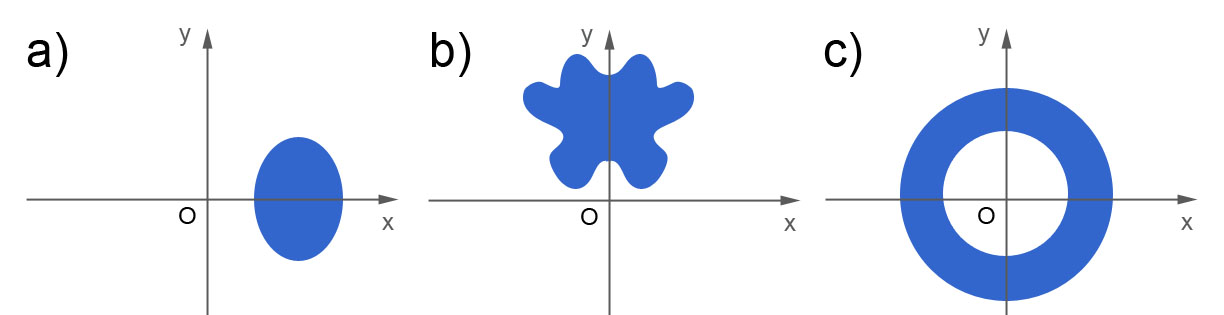
\includegraphics[width=0.95\textwidth]{ImgRegions.jpg}
  \end{center}
 \begin{quote} \caption{\small{a) the blue region is symmetric about the $x$-axis, b) the blue region is symmetric about the $y$-axis, and c) the blue region is symmetric about the $x$-axis and the $y$-axis.}}\end{quote}
\end{figure}

Moreover, if $g(x,y)$ is odd in $x$, then 
\begin{align*}
  g(-x,y) = - g(x,y).
\end{align*}
But if $g(x,y)$ were even in $x$, then 
\begin{align*}
  g(-x,y) =  g(x,y).
\end{align*}
Combining these concepts yields helpful results for computing double integrals. For example, if $R$ is symmetric about the $y$-axis, and if $g(x,y)$ is odd in $x$, then
\begin{align*}
  \iint\limits_R g(x,y) dxdy = 0.
\end{align*}
Similar results can be stated if $g$ were even in $x$ or in $y$, and if $R$ has symmetry about the $x$-axis. 
\BEN
\item Provide an example of a non-zero function of two variables, $h(x,y)$, that is odd in $x$. Verify that your function is odd in $x$.
\item Provide an example of a region, $D$, that is symmetric about the $y$-axis, but is not symmetric about the $x$-axis. 
\item Show that, for your $h(x,y)$ and region $D$, that 
\begin{align*}
  \iint\limits_D g(x,y) dxdy = 0.
\end{align*}
\EEN

\EEN % END OF SUBSECTION
% s~s~s~s~s~s~s~s~s~s~s~s~s~s~s~s~s~s~s~s~s~s~s~s~s~s~s~s~s~s~s~s~s~s~s~s~s~s~s~s~s~s~s~s
% s~s~s~s~s~s~s~s~s~s~s~s~s~s~s~s~s~s~s~s~s~s~s~s~s~s~s~s~s~s~s~s~s~s~s~s~s~s~s~s~s~s~s~s

\subsection{Triple Integrals}
\purple{\From Section 3.3 of \VCT.}
  
\BEN
% ~~~~~~~~~~~~~~~~~~~~~~~~~~~~~~~~~~~~~~~~~~~~~~~~~~~~~~~~~~~~~~~~~~~~~~~~~~~~~~~~~
\item % TETRAHEDRON
\Emph{Volume of a Tetrahedron} \\
The textbook points out that the triple integral 
\begin{align*}
  \iiint\limits_S f(x,y,z) dV
\end{align*}
for the special special case when $f(x,y,z) = 1$ for all points in $S$, gives the volume of $S$
\begin{align*}
  V(S) &= \iiint\limits_S dV.
\end{align*}
Consider again the tetrahedron that is bounded by the three coordinate planes in $\R^3$, and by the plane $z = 1 - x - \frac{y}{2}$. We derived an expression for the volume of this tetrahedron in a previous question using a double integral. Now set-up and find the volume of the tetrahedron using a triple integral.
% ~~~~~~~~~~~~~~~~~~~~~~~~~~~~~~~~~~~~~~~~~~~~~~~~~~~~~~~~~~~~~~~~~~~~~~~~~~~~~~~~~
\item % VOLUME OF AN ELLIPSOID
\textbf{Volume of an Ellipsoid}\\
Solve Question 10 from Section 3.5 of \VCT.
% ~~~~~~~~~~~~~~~~~~~~~~~~~~~~~~~~~~~~~~~~~~~~~~~~~~~~~~~~~~~~~~~~~~~~~~~~~~~~~~~~~
\item % VOLUME OF SOLID
\textbf{Volume of a Solid}\\
Find the volume of the solid enclosed by the planes
\begin{align*}
  z & = x+y\\
  y &= x \\
  x &= 0 \\
  z &= -1 \\
  y &= 2
\end{align*}
\textit{Hint: it may help to start by plotting the planes in Google or in Wolfram Alpha.}\\
\rednote{The solutions need to be adjusted so that z is in -1 to x+y}
\EEN % END OF SUBSECTION
% s~s~s~s~s~s~s~s~s~s~s~s~s~s~s~s~s~s~s~s~s~s~s~s~s~s~s~s~s~s~s~s~s~s~s~s~s~s~s~s~s~s~s~s
% s~s~s~s~s~s~s~s~s~s~s~s~s~s~s~s~s~s~s~s~s~s~s~s~s~s~s~s~s~s~s~s~s~s~s~s~s~s~s~s~s~s~s~s
\subsection{Change of Variables in Multiple Integrals}
\purple{\From Section 3.5 of \VCT.}
\BEN
% ~~~~~~~~~~~~~~~~~~~~~~~~~~~~~~~~~~~~~~~~~~~~~~~~~~~~~~~~~~~~~~~~~~~~~~~~~~~~~~~~~
\item % GENERAL TRANSFORMATION
\Emph{Linear Transformations} \\
Under the linear transformation 
\begin{align*}
  x = c_1u + c_2v , \quad y =d_1u + d_2v, \quad d_1c_2 - d_2c_1 \ne 0,
\end{align*}
straight lines in the $uv$-plane are mapped to straight lines in the $xy$-plane. 
\BEN
\item $v=v_0$ is a horizontal line in the $uv$-plane. Determine the equation of this line in the $xy$-plane. 
\item $x=x_0$ is a vertical line in the $xy$-plane. Determine the equation of this line in the $uv$-plane.
\EEN
% ~~~~~~~~~~~~~~~~~~~~~~~~~~~~~~~~~~~~~~~~~~~~~~~~~~~~~~~~~~~~~~~~~~~~~~~~~~~~~~~~~
\item % STRAIGHTFORWARD CHANGE OF VARIABLES
Use an appropriate transformation to evaluate the integral
\begin{align*}
  \iint\limits_R \big(x^2 - y^2\big) dxdy,
\end{align*}
where $R$ is the parallelogram bounded by 
\begin{align*}
  x+y = 0, \quad x+y = 1, \quad x-y=0, \quad x-y=1.
\end{align*}

% ~~~~~~~~~~~~~~~~~~~~~~~~~~~~~~~~~~~~~~~~~~~~~~~~~~~~~~~~~~~~~~~~~~~~~~~~~~~~~~~~~
\item % CHANGE OF VARIABLES TWICE
\Emph{Simplifying Double Integrals} \\
When working with double integrals over a rectangular region $R=\{(x,y) | a \le x \le b, c\le y \le d\}$, we can use the simplification
\begin{align*}
   \iint\limits_{R} g(x) h(y) dA 
  & = \int_a^b g(x) dx \int_c^d h(y) dy  
\end{align*}
Use this property and the transformation $x = 3u, y = 2v$ to evaluate the double integral
\begin{align*}
  \iint\limits_E x^2 \ dxdy,
\end{align*}
where $E$ is region bounded by the ellipse $4x^2 + 9y^2 = 36$. 
% ~~~~~~~~~~~~~~~~~~~~~~~~~~~~~~~~~~~~~~~~~~~~~~~~~~~~~~~~~~~~~~~~~~~~~~~~~~~~~~~~~
\item % SIMPLE CYLINDRICAL WITH CONE
Evaluate the integral
\begin{align*}
  \iiint\limits_S y^2dV,
\end{align*}
where $S$ is the solid that lies inside the cylinder $x^2+y^2 = 1$, above the plane $z=0$ and below the cone $z^2 = 9x^2 + 9y^2$. 
% ~~~~~~~~~~~~~~~~~~~~~~~~~~~~~~~~~~~~~~~~~~~~~~~~~~~~~~~~~~~~~~~~~~~~~~~~~~~~~~~~~
\item % TRIPLE INTEGRAL IN CYLINDRICAL COORDINATES
\Emph{Triple Integral In Cylindrical Coordinates} \\
Evaluate the integral
\begin{align*}
  \iiint\limits_V dV,
\end{align*}
using cylindrical coordinates, where $V$ is the region bounded by
\begin{align*}
  0 \le\ &x \le 2 \\
  0 \le\ &y \le \sqrt{4 - x^2}\\
  0 \le\ &z \le \sqrt{4 - (x^2+ y^2)}
\end{align*} 
% ~~~~~~~~~~~~~~~~~~~~~~~~~~~~~~~~~~~~~~~~~~~~~~~~~~~~~~~~~~~~~~~~~~~~~~~~~~~~~~~~~
\item % TRIPLE INTEGRAL IN SPHERICAL COORDINATES
\Emph{Triple Integral In Spherical Coordinates} \\
The integral
\begin{align*}
  \mathop{\int_0^{\pi/4} \!\! \int_{0}^{\pi/2} \!\! \int_0^1 } ( \rho^2 \sin\phi ) \ d\rho\  d\phi\  d\theta
\end{align*}
represents the volume of a solid. Describe the shape of the solid, and find its volume. \\\rednote{Textbook doesn't do a great job of integrals in cylindrical and spherical}
% ~~~~~~~~~~~~~~~~~~~~~~~~~~~~~~~~~~~~~~~~~~~~~~~~~~~~~~~~~~~~~~~~~~~~~~~~~~~~~~~~~
\EEN % END OF SUBSECTION 
% s~s~s~s~s~s~s~s~s~s~s~s~s~s~s~s~s~s~s~s~s~s~s~s~s~s~s~s~s~s~s~s~s~s~s~s~s~s~s~s~s~s~s~s
% s~s~s~s~s~s~s~s~s~s~s~s~s~s~s~s~s~s~s~s~s~s~s~s~s~s~s~s~s~s~s~s~s~s~s~s~s~s~s~s~s~s~s~s
\subsection{Application: Center of Mass}
\purple{\From Section 3.6 of \VCT.}
\BEN
% ~~~~~~~~~~~~~~~~~~~~~~~~~~~~~~~~~~~~~~~~~~~~~~~~~~~~~~~~~~~~~~~~~~~~~~~~~~~~~~~~~
\item % CENTER OF MASS OF 2D TRIANGULAR PLATE
\Emph{Center of Mass of a 2D Triangular Plate} \\
A two-dimensional plate has density $\delta(x,y) = xy$, and occupies a triangular region whose vertices are located at the points (0,0), (1,2), and (1,4). Find the $x$-coordinate and the $y$-coordinate of the center of mass of the triangular plate. 
% ~~~~~~~~~~~~~~~~~~~~~~~~~~~~~~~~~~~~~~~~~~~~~~~~~~~~~~~~~~~~~~~~~~~~~~~~~~~~~~~~~
\item % CENTER OF MASS OF 2D RADIAL DENSITY FUNCTION
\Emph{Center of Mass of a 2D Plate, Radial Density Function} \\
A 2D semi-circular plate of mass $M$ is bounded by 
\begin{align*}
  -a \le x \le a, \quad 0 \le y \le \sqrt{a^2 - x^2}, \quad a > 0.
\end{align*}
The density of the plate at a point $(x,y)$, is equal to the shortest distance, $L$, between that point and the upper edge of the plate, as shown in Figure \ref{FigCircPlate}. 
\BEN
\item Set up an integral that represents the $x$-coordinate of the center of mass of the plate, $\bar{x}$. 
\item Set up an integral that represents the $y$-coordinate of the center of mass of the plate, $\bar{y}$. 
\item Determine the $x$-coordinate of the center of mass of the plate, without performing any integration. Briefly describe how you found your answer. 
\EEN
You do not need to perform any integration for this question. Note also that $L$ is a function of $x$ and $y$. 
\begin{figure}[H]
  \vspace{-1pt}
  \begin{center}
    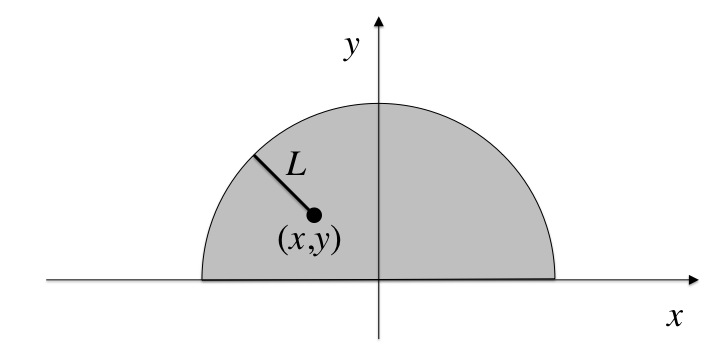
\includegraphics[width=0.65\textwidth]{ImgRadialCenterOfMass.jpg}
  \end{center}
 \begin{quote} \caption{\label{FigCircPlate}\small{The density of the plate at $(x,y)$ is equal to $L$.}}\end{quote}
\end{figure}
% ~~~~~~~~~~~~~~~~~~~~~~~~~~~~~~~~~~~~~~~~~~~~~~~~~~~~~~~~~~~~~~~~~~~~~~~~~~~~~~~~~
\item % MOMENTS OF A CYLINDER
\Emph{Center of Mass of a 2D Plate, Radial Density Function} \\

% ~~~~~~~~~~~~~~~~~~~~~~~~~~~~~~~~~~~~~~~~~~~~~~~~~~~~~~~~~~~~~~~~~~~~~~~~~~~~~~~~~
\item % EVEN AND ODD
\rednote{I'll push this question to a midterm or final exam}\\
Determine the value of
\begin{align*}
  \mathop{\int_0^{\pi} \!\! \int_{-1}^1} x^4e^{x^2 + y^2}\sin(y) dydx.
\end{align*}
Do not use integration by parts.
% ~~~~~~~~~~~~~~~~~~~~~~~~~~~~~~~~~~~~~~~~~~~~~~~~~~~~~~~~~~~~~~~~~~~~~~~~~~~~~~~~~
\EEN % END OF SUBSECTION 







% ~~~~~~~~~~~~~~~~~~~~~~~~~~~~~~~~~~
% SOLUTIONS
\newpage
\part{Solutions to Written Assignment Questions}
\setcounter{section}{1}

\section{Multivariable Functions and Algebra}
\subsection{Dot Products and Cross Products}
\BEN

%% ~~~~~~~~~~~~~~~~~~~~~~~~~~~~~~~~~~~~~~~~~~~~~~~~~~~~~~~~~
%\item
%\begin{enumerate}
%\item 
%
%A vector parallel to the required line is given by $\BM 3\\ -2\\1\EM - \BM -1 \\2 \\ 1\EM  = \BM 4 \\-4 \\0 \EM$. If we like, for simplicity, we can normalize this vector by dividing each component by 4 to obtain the vector $[1,-1,0]^T$. Since a point on the desired line is (-1,2,1), a vector equation is given by 
%\begin{align*}
%\mathbf{r}=\BM-1 \\2 \\1\EM+t\BM1 \\ -1 \\0 \EM.
%\end{align*}
%The solution to this question is not unique. Any vector parallel to the vector $\BM 4 \\ -4 \\ 0 \EM$ could be used. 
%
%% -  -  -  -  -  -  -  -  -  -  -  -  -  -  -  -  -  -  -  -  -  -  -  -  -  -  -  -  -  -  
%\item 
%A vector equation is 
%\begin{align*}
%\mathbf{r} &= (2+2t)\mathbf{i} + (9t)\mathbf{j} + (5+t)\mathbf{k} \\
%&= (2\mathbf{i} + 5\mathbf{k}) + t(2\mathbf{i} + 9\mathbf{k} + \mathbf{k}) \\
%&= \BM 2 \\ 0 \\ 5 \EM + t \BM 2 \\ 9 \\1 \EM
%\end{align*}
%\end{enumerate}
%% ~~~~~~~~~~~~~~~~~~~~~~~~~~~~~~~~~~~~~~~~~~~~~~~~~~~~~~~~~
%\item
%% -  -  -  -  -  -  -  -  -  -  -  -  -  -  -  -  -  -  -  -  -  -  -  -  -  -  -  -  -  -  
%\begin{enumerate}
%\item 
%Let $\mathbf{A} = \BM-1 \\ 0 \\ 1\EM$ and $\mathbf{B} = \BM 0 \\ -2 \\ 2 \EM$. Then
%\begin{align*}
%  \mathbf{A} \cdot \mathbf{B} &= \big((-1)(0)\big) + \big((0)(-2)\big) + \big((1)(2)\big)\\
%  &= 0 + 0 + 2 \\
%  &= 2
%\end{align*}
%Also,
%\begin{align*}
%  || \mathbf{A} || &= \sqrt{(-1)^2 + 0 + (1)^2} = \sqrt{2} \\
%  || \mathbf{B} || &= \sqrt{0^2 + (-2)^2 + 2^2} = \sqrt{8}
%\end{align*}
%Therefore, if $\theta$ is the angle between the two vectors, 
%\begin{align*}
%  \cos\theta &= \frac{ \mathbf{A}\cdot \mathbf{B}}{|| \mathbf{A}|| \ || \mathbf{B}||} = \frac{2}{4} = \frac{1}{2}
%\end{align*}
%Therefore, $\theta = \pi/3$. 
%
%% -  -  -  -  -  -  -  -  -  -  -  -  -  -  -  -  -  -  -  -  -  -  -  -  -  -  -  -  -  -  
%\item 
%Let the vector perpendicular to the plane be $\mathbf{y}= \BM 2 \\ 1 \\ -1 \EM$. The angle, $\theta$, between the given vector and $\mathbf{y}$ is found by solving
%\begin{align*}
%  \cos\theta &= \frac{ \mathbf{x}\cdot \mathbf{y}}{|| \mathbf{x}|| \ || \mathbf{y}||} \\
%  &= \frac{ \BM 1 \\0 \\ 2 \EM \cdot \BM 2 \\1 \\-1 \EM} {\sqrt{5}\sqrt{6}}\\
%    &= \frac{ 0 } {\sqrt{5}\sqrt{6}}\\
%    &=0.
%\end{align*}
%The angle, $\theta$, is $\pi/2$. But $\theta$ is the angle between $\mathbf{x}$ and $\mathbf{y}$ and we need the angle between $\mathbf{x}$ and the plane, which is $\pi/2 - \theta = 0$. Therefore, the desired angle is 0 (the given vector is parallel to the plane). 
%\end{enumerate}
%
%% ~~~~~~~~~~~~~~~~~~~~~~~~~~~~~~~~~~~~~~~~~~~~~~~~~~~~~~~~~
%\item
%Let the normal vector of the first plane be $\mathbf{n}_1$, and the normal vector of the second plane be $\mathbf{n}_2$. Then  
%\begin{align*}
%\mathbf{n}_1 \times \mathbf{n}_2 
%&= (0-(-8))\mathbf{i} - (1-4)\mathbf{j}+(-2-0)\mathbf{k} \\
%&=\BM 8 \\ 3 \\ -2 \EM
%\end{align*}
%This vector is perpendicular to the two given vectors. Its length is
%\begin{align*}
%\big|\big| [8,3,-2]^T \big|\big| 
%&= \sqrt{ 8^2+3^2+(-2)^2} \\
%&= \sqrt{77}
%\end{align*}
%Therefore, two unit vectors are
%\begin{align*}
%\BM 8/\sqrt{77} \\ 3/\sqrt{77}\\ -2/\sqrt{77}\EM , \text{ and } \BM -8/\sqrt{77} \\ -3/\sqrt{77} \\ 2/\sqrt{77} \EM
%\end{align*}
%% ~~~~~~~~~~~~~~~~~~~~~~~~~~~~~~~~~~~~~~~~~~~~~~~~~~~~~~~~~
%\item
%The formula we can apply is:
%\begin{align*}
%  D = \frac{||\mathbf{v} \times \mathbf{w}||}{|| \mathbf{v}||}
%\end{align*}
%where $\mathbf{v}$ is a vector parallel to the given line, and is
%\begin{align*}
%  \mathbf{v} &= \BM 0 \\ 1 \\ 0 \EM.
%\end{align*}
%The vector $\mathbf{w}$ is
%\begin{align*}
%  \mathbf{w} &= \BM 1 \\ 0 \\ 0 \EM  - \BM 1 \\ 0 \\ 1 \EM = \BM 0\\0\\-1 \EM
%\end{align*}
%Then,
%\begin{align*}
%  D & = \frac{||\mathbf{v} \times \mathbf{w}||}{|| \mathbf{v}||} \\
%  &= \frac{||[ -1,0,0 ] ^T||}{|| [0,1,0]^T||}\\
%  &= \frac{1}{1}\\
%  &= 1
%\end{align*}
%% ~~~~~~~~~~~~~~~~~~~~~~~~~~~~~~~~~~~~~~~~~~~~~~~~~~~~~~~~~
%\item 
%The formula we can apply is:
%\begin{align*}
%  D = \frac{| ax_0 + by_0 +cz_0 +d|}{\sqrt{a^2+b^2+c^2}}
%\end{align*}
%where $a, b, c$ are the components of the normal vector to the plane, so that
%\begin{align*}
%  \BM a \\ b \\ c \EM = \BM 2 \\ 1 \\ -1 \EM
%\end{align*}
%The point $(x_0,y_0,z_0) = (-1 , C, 1)$, $d = -3$, and $D = \sqrt{6}$. Thus,
%\begin{align*}
%  D = \sqrt{6} &= \frac{| 2(-1) + C(1) + (1)(-1) -3|}{\sqrt{6}}\\
%  &= \frac{| C - 6|}{\sqrt{6}}\\
%  1 &= | C - 6| \\
%\end{align*}
%Therefore, $C = 5, 7$.
% ~~~~~~~~~~~~~~~~~~~~~~~~~~~~~~~~~~~~~~~~~~~~~~~~~~~~~~~~~
%\item  % SOLUTION
%\begin{enumerate}
%\item
%We can start by finding the plane that contains the three points. The vectors $\overrightarrow{PQ}$ and $\overrightarrow{PR}$ are 
%
%\begin{align*}
%\overrightarrow{PQ} &= \BM 2 \\ 2 \\ 3 \EM - \BM 1 \\ 0 \\ 3 \EM  = \BM 1 \\ 2 \\ 0 \EM \\
%\overrightarrow{PR} &= \BM 0 \\ 0 \\ -1 \EM - \BM 1 \\ 0 \\ 3 \EM  =  \BM -1 \\ 0 \\ -4 \EM
%\end{align*}
%
%A vector perpendicular to the plane that contains the three points is found by calculating the cross product between these two vectors:
%\begin{align*}
%\overrightarrow{PQ} \times \overrightarrow{PR} 
%&= (-8-(0))\mathbf{i} - (-4-0)\mathbf{j}+(0-(-2))\mathbf{k} \\
%&= \BM -8 \\ 4 \\ 2 \EM
%\end{align*}
%Any vector parallel to this vector is perpendicular to the plane that contains the given points. 
%% -  -  -  -  -  -  -  -  -  -  -  -  -  -  -  -  -  -  -  -  -  -  -  -  -  -  -  -  -  -  
%\item
%To find the area, $A$, of  triangle $\bigtriangleup PQR$, we can use a cross product.
%\begin{align*}
%A &= \frac{1}{2} \big|\big| \overrightarrow{PQ} \times \overrightarrow{PR} \big|\big| \\
%&= \frac{1}{2} \big|\big| [-8,4,2]^T \big|\big| \\
%&= \frac{1}{2} \sqrt{ (-8)^2+4^2+2^2} \\
%&= \frac{1}{2} \sqrt{ 84} \ \\
%&= \sqrt{21} \\
%\end{align*}
%% -  -  -  -  -  -  -  -  -  -  -  -  -  -  -  -  -  -  -  -  -  -  -  -  -  -  -  -  -  -  
%\item
%If the point $S$ is such that $\overrightarrow{PQ}$ is parallel to $\overrightarrow{QS}$, then there will be an infinite number of planes that pass through these three points. Such a point, $S$, can be determined by multiplying $\overrightarrow{PQ}$ by a constant. Choosing 2 as a constant, then 
%\begin{align*}
%\overrightarrow{QS} &= \BM 2 \\ 4 \\ 0 \EM\\
%\end{align*}
%We determine the components of $S$ as
%\begin{align*}
%S &= \BM 2-2 \\ 4-2 \\ 0-3 \EM = \BM 0 \\ 2 \\ -3 \EM\\
%\end{align*}
%\end{enumerate}

% ~~~~~~~~~~~~~~~~~~~~~~~~~~~~~~~~~~~~~~~~~~~~~~~~~~~~~~~~~
\item
\rednote{Where did the solution go?}
% ~~~~~~~~~~~~~~~~~~~~~~~~~~~~~~~~~~~~~~~~~~~~~~~~~~~~~~~~~

\item
It is not necessarily true that $\mathbf{b}=\mathbf{c}$. Simple rearrangement yields
\begin{align*}
\mathbf{a}\cdot\mathbf{b}&=\mathbf{a}\cdot\mathbf{c} \\
0 &=\mathbf{a}\cdot\mathbf{b} - \mathbf{a}\cdot\mathbf{c} \\
0 &=\mathbf{a}\cdot (\mathbf{b} - \mathbf{c})
\end{align*}
Therefore, \textbf{a} is perpendicular to the vector $\mathbf{b} - \mathbf{c}$, which can be true when $\mathbf{b} \ne \mathbf{c}$.  A counterexample would be the vectors
\begin{align*}
\mathbf{a} = \BM 1 \\ 1 \\ 0 \EM ,  \quad \mathbf{b} = \BM 1 \\ -1 \\ 0 \EM , \quad  \mathbf{c} = \BM 0 \\ 0 \\ 0 \EM .
\end{align*}
Clearly, \textbf{a}$\cdot\mathbf{b}=\mathbf{a}\cdot\mathbf{c}$, even though $\mathbf{b} \ne \mathbf{c}$.  
% ~~~~~~~~~~~~~~~~~~~~~~~~~~~~~~~~~~~~~~~~~~~~~~~~~~~~~~~~~
%
%\item
%\begin{enumerate}
%\item
%Let the points $P, Q, R$ be \\
%\begin{align*}
%P &=(-1,2,1)\\
%Q &=(3,-2,1)\\
%R &=(-1,1,-1)
%\end{align*}
%Vectors  $\overrightarrow{PQ}$ and $\overrightarrow{PR}$ are
%\begin{align*}
%\overrightarrow{PQ} &= \BM 3 \\ -2 \\ 1 \EM -(-1,2,1) = (4,-4,0)\\
%\overrightarrow{PR} &= \BM -1 \\ 1 \\ -1 \EM - \BM -1 \\ 2 \\ 1 \EM = \BM 0 \\ -1 \\ -2\EM
%\end{align*}
%A vector orthogonal to the plane that contains the three points is found by calculating the cross product between these two vectors:
%\begin{align*}
%\overrightarrow{PQ} \times \overrightarrow{PR} 
%&= (8-0)\mathbf{i} - (-8-0)\mathbf{j}+(-4-0)\mathbf{k} \\
%&=(8,8,-4)
%\end{align*}
%The equation of the desired plane, using the point-normal form, is
%\begin{align*}
%0&=8(x+1)+8(y-2)+(-4)(z-1)\\
%4&=8x + 8y -4z
%\end{align*}
%
%\item
%The points $(0,0,0)$ and $(1,1,1)$ are on the given line. Therefore, the vector $\BM 1 \\ 1 \\1 \EM$ is parallel to the desired plane. Another vector parallel to the desired plane is 
%\begin{align*}
%  \BM -1 \\ 2 \\ 1 \EM - \BM 0 \\ 0 \\0 \EM = \BM -1\\2\\1\EM.
%\end{align*}
%Therefore, a vector perpendicular to the desired plane is 
%\begin{align*}
%\BM 1\\1\\1\EM  \times \BM-1\\2\\1\EM 
%&= (1-2)\mathbf{i} - (1+1)\mathbf{j}+(2+1)\mathbf{k} = \BM -1 \\ -2 \\ 3 \EM .
%\end{align*}
%The equation of the desired plane, using the point-normal form, is
%\begin{align*}
%0&=-1(x+1)-2(y-2)+3(z-1)\\
%0 &=-x - 2y +3z .
%\end{align*}
%
%
%\end{enumerate}
%% ~~~~~~~~~~~~~~~~~~~~~~~~~~~~~~~~~~~~~~~~~~~~~~~~~~~~~~~~~
%% EQUATION OF PLANE FROM INTERSECTION BETWEEN TWO LINES
%\item
%
%Let the normal vector of the first plane be $\mathbf{n}_1$, and the normal vector of the second plane be $\mathbf{n}_2$. Then  
%\begin{align*}
%\mathbf{n}_1 =\BM 2 \\ 1 \\ -1 \EM, \ 
%\mathbf{n}_2=\BM 1\\ 3 \\ 1 \EM
%\end{align*}
%The line that intersects these two planes is a line that is in both of the planes, and therefore must be perpendicular to both $\mathbf{n}_1$ and $\mathbf{n}_2$. Therefore, the line we need is parallel to the vector, $\mathbf{a}$, given by the cross product
%\begin{align*}
%\mathbf{a} &= \mathbf{n}_1 \times \mathbf{n}_2 = (4,-3,5).
%\end{align*}
%This vector is parallel to the desired plane. To find a second vector in the desired plane, we can find a line from the given point to any point in the line of intersection of the two given planes. Letting $y=0$, we obtain the equations
%\begin{align*}
%2x-z&=3\\
%x+z&=0
%\end{align*}
%which has the solution $x=1, z=-1$. Therefore, the point $(1,0,-1)$ is in the intersection of the two planes, and a vector in the plane is
%\begin{align*}
%\BM 1 \\ 0 \\ -1 \EM- \BM 0 \\ 0 \\ 0 \EM = \BM 1 \\ 0 \\ -1 \EM.
%\end{align*}
%A normal vector to the desired plane is 
%\begin{align*}
%[1,0,-1]^T \times [4,-3,5]^T 
%&= (0-3)\mathbf{i} - (5+4)\mathbf{j}+(-3-0)\mathbf{k} \\
%&=-3\mathbf{i} -9 \mathbf{j} -3\mathbf{k} 
%\end{align*}
%The equation of the desired plane, using the point-normal form, is
%\begin{align*}
%0&=(-3)(x-0)+(-9)(y-0)+(-3)(z-0)\\
%&=-3x-9y-3z
%\end{align*}
%
%% ~~~~~~~~~~~~~~~~~~~~~~~~~~~~~~~~~~~~~~~~~~~~~~~~~~~~~~~~~
%% ORTHOGONAL VECTORS
%\item
%\begin{enumerate}
%% ~ ~ ~ ~ ~ ~ ~ ~ ~ ~ ~ ~ ~ ~ ~ ~ ~ ~ ~ ~ ~ ~ ~ ~ ~ ~ ~ ~ ~ ~ ~ ~ ~ ~ ~ ~ ~ ~ ~ ~ 
%% PART A
%\item We will show that the two lines must be equal to each other, and therefore share an infinite number of points. Let $P$ be the common point, and $\mathbf{r}$ be the vector pointing from the origin to the point $P$. Let 
%\begin{align*}
%  L_1 &= \mathbf{r} + t\mathbf{u} \\
%  L_2 &= \mathbf{r} + t\mathbf{v} \\  
%\end{align*}
%where $t \in \R$, and \textbf{u} and \textbf{v} are vectors parallel to the lines $L_1$ and $L_2$ respectively. Let their components be 
%\begin{align*}
%\mathbf{u} = \begin{bmatrix} u_1 \\ u_2 \\ u_3 \end{bmatrix},  \quad
%\mathbf{v} = \begin{bmatrix} v_1 \\ v_2 \\ v_3 \end{bmatrix} .
%\end{align*}
%When the lines intersect, their components are equal, which gives us the three equations 
%\begin{align*}
%r_1 +t u_1 &= r_1 + tv_1 \\
%r_2 +t u_2 &= r_2 + tv_2 \\
%r_3 +t u_3 &= r_3 + tv_3 
%\end{align*}
%Or simply
%\begin{align*}
%t u_1 &= tv_1 \\
%t u_2 &= tv_2 \\
%t u_3 &= tv_3 
%\end{align*}
%Because $L_1$ and $L_2$ are parallel, vectors \textbf{u} and \textbf{v} must also be parallel. Therefore $\mathbf{u}=k\mathbf{v}$ where $k$ is a constant, so 
%\begin{align*}
%t u_1 &= tku_1 \\
%t u_2 &= tku_2 \\
%t u_3 &= tku_3 
%\end{align*}
%These equations are only satisfied if $k=1$. Therefore, the two lines must be equal to each other, implying that there an infinite number of points that the two lines share. 
%% ~ ~ ~ ~ ~ ~ ~ ~ ~ ~ ~ ~ ~ ~ ~ ~ ~ ~ ~ ~ ~ ~ ~ ~ ~ ~ ~ ~ ~ ~ ~ ~ ~ ~ ~ ~ ~ ~ ~ ~ 
%% PART B
%\item Yes. Any plane in $\R^3$ can be expressed in point-normal form 
%\begin{align*}
%a(x-x_0) - b(y-y_0)+c(z-z_0) = 0
%\end{align*}
%where the vector $\begin{bmatrix} a \\ b \\ c \end{bmatrix}$ is a vector normal to the plane. 
%\end{enumerate}

% ~~~~~~~~~~~~~~~~~~~~~~~~~~~~~~~~~~~~~~~~~~~~~~~~~~~~~~~~~
% ORTHOGONAL VECTORS
\item
\begin{enumerate}
% ~ ~ ~ ~ ~ ~ ~ ~ ~ ~ ~ ~ ~ ~ ~ ~ ~ ~ ~ ~ ~ ~ ~ ~ ~ ~ ~ ~ ~ ~ ~ ~ ~ ~ ~ ~ ~ ~ ~ ~ 
% PART A
\item Vectors $\mathbf{a}$ and $\mathbf{b}$ are perpendicular because their dot product is zero:
\begin{align*}
\mathbf{a} \cdot \mathbf{b} = \frac{1}{2} -  \frac{1}{2} =0.
\end{align*}
Vectors $\mathbf{a}$ and $\mathbf{b}$ are both unit vectors, because they have length 1:
\begin{align*}
|| \mathbf{a} || &=  \sqrt{ \Bigg( \frac{1}{\sqrt{2}}\Bigg)^2 +  \Bigg(\frac{-1}{\sqrt{2}}\Bigg)^2} = 1\\
|| \mathbf{b} || &=  \sqrt{ \Bigg( \frac{1}{\sqrt{2}}\Bigg)^2 +  \Bigg(\frac{1}{\sqrt{2}}\Bigg)^2} = 1
\end{align*}
% ~ ~ ~ ~ ~ ~ ~ ~ ~ ~ ~ ~ ~ ~ ~ ~ ~ ~ ~ ~ ~ ~ ~ ~ ~ ~ ~ ~ ~ ~ ~ ~ ~ ~ ~ ~ ~ ~ ~ ~ 
% PART B
\item Using results from part (a), we can find $C_1$ as follows:
\begin{align*}
\mathbf{r} &= C_1 \mathbf{a} + C_2  \mathbf{b} \\
\mathbf{a}\cdot\mathbf{r} &=  \mathbf{a}\cdot \Big(C_1 \mathbf{a} + C_2 \mathbf{b} \Big)\\
\mathbf{a}\cdot\mathbf{r} &= C_1 \mathbf{a}\cdot \mathbf{a} + C_2\mathbf{a}\cdot   \mathbf{b} \\
\frac{2}{\sqrt{2}} &= C_1 (1) + C_2(0) \\
C_1 &= \frac{2}{\sqrt{2}} \\
\end{align*}
A similar calculation yields $C_2$
\begin{align*}
\mathbf{r} &= C_1 \mathbf{a} + C_2  \mathbf{b} \\
\mathbf{b}\cdot\mathbf{r} &=  \mathbf{b}\cdot \Big(C_1 \mathbf{a} + C_2 \mathbf{b} \Big)\\
\mathbf{b}\cdot\mathbf{r} &= C_1 \mathbf{b}\cdot \mathbf{a} + C_2\mathbf{b}\cdot   \mathbf{b} \\
\frac{4}{\sqrt{2}} &= C_1 (0) + C_2(1) \\
C_2 &= \frac{4}{\sqrt{2}} = 2\sqrt{2} \\
\end{align*}
\end{enumerate}
% ~~~~~~~~~~~~~~~~~~~~~~~~~~~~~~~~~~~~~~~~~~~~~~~~~~~~~~~~~
% TRUE/FALSE
\item
% ~ ~ ~ ~ ~ ~ ~ ~ ~ ~ ~ ~ ~ ~ ~ ~ ~ ~ ~ ~ ~ ~ ~ ~ ~ ~ ~ ~ ~ ~ ~ ~ ~ ~ ~ ~ ~ ~ ~ ~ 
% PART A
\begin{enumerate}
\item Expanding the left-hand side yields
\begin{align*}
||\mathbf{a} + \mathbf{b}||^2 &= \big(\mathbf{a} + \mathbf{b}\big)\cdot\big(\mathbf{a} + \mathbf{b}\big) \\
&= \mathbf{a}\cdot\mathbf{a} + \mathbf{b}\cdot\mathbf{b} + 2\mathbf{a}\cdot\mathbf{b}\\
&= ||\mathbf{a}||^2 + ||\mathbf{b}||^2 + 2\mathbf{a}\cdot\mathbf{b}
\end{align*}
This is equal to $ ||\mathbf{a}||^2 + ||\mathbf{b}||^2$ iff $\mathbf{a}\cdot\mathbf{b}=0$, which implies that $\mathbf{a}$ must be perpendicular to $\mathbf{b}$.
% ~ ~ ~ ~ ~ ~ ~ ~ ~ ~ ~ ~ ~ ~ ~ ~ ~ ~ ~ ~ ~ ~ ~ ~ ~ ~ ~ ~ ~ ~ ~ ~ ~ ~ ~ ~ ~ ~ ~ ~ 
\item First consider the dot product:
\begin{align*}
\mathbf{a}\cdot\mathbf{b} &= \mathbf{a}\cdot\mathbf{c} \\
0 &= \mathbf{a}\cdot\mathbf{b} - \mathbf{a}\cdot\mathbf{c} \\
0 &= \mathbf{a}\cdot\big(\mathbf{b} - \mathbf{c}\big) \\
\end{align*}
Therefore, $\mathbf{a}$ is perpendicular to the vector $\mathbf{b} - \mathbf{c}$. Manipulation of the cross product yields
\begin{align*}
\mathbf{a}\times\mathbf{b} &= \mathbf{a}\times\mathbf{c} \\
0 &= \mathbf{a}\times\mathbf{b} - \mathbf{a}\times\mathbf{c} \\
0 &= \mathbf{a}\times\big(\mathbf{b} - \mathbf{c}\big) \\
\end{align*}
Therefore, $\mathbf{a}$ is also parallel to the vector $\mathbf{b} - \mathbf{c}$. Therefore, $\mathbf{b} - \mathbf{c} = \mathbf{0}$, or $\mathbf{b} = \mathbf{c}$.
%\item The statement is false: $\BM 1 \\ 2 \\ 3 \EM = \BM 1 ,2 ,3\EM^T$.
% ~ ~ ~ ~ ~ ~ ~ ~ ~ ~ ~ ~ ~ ~ ~ ~ ~ ~ ~ ~ ~ ~ ~ ~ ~ ~ ~ ~ ~ ~ ~ ~ ~ ~ ~ ~ ~ ~ ~ ~ 
\end{enumerate}
% ~~~~~~~~~~~~~~~~~~~~~~~~~~~~~~~~~~~~~~~~~~~~~~~~~~~~~~~~~
% MEANINGLESS STATEMENTS
\item
\begin{enumerate}
\item This statement is not meaningless. This is a dot product of two vectors.
\item This statement is meaningless. We cannot take the dot product of a vector with a scalar. 
\item This statement is meaningless. We cannot take the cross product of a vector with a scalar. 
\item This statement is not meaningless. This is a cross product of two vectors.
\end{enumerate}
% ~~~~~~~~~~~~~~~~~~~~~~~~~~~~~~~~~~~~~~~~~~~~~~~~~~~~~~~~~
% TORQUE
\item
For this problem we will use the coordinate system in the diagram below. 
\begin{figure}[!htbp]
  \begin{center}
    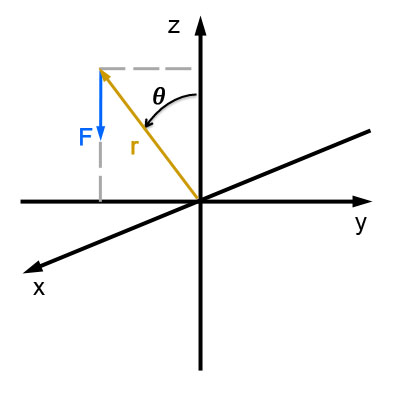
\includegraphics[width=0.4\textwidth]{ImgTorqueSol.jpg}
  \end{center}
\end{figure}
\BEN
\item Using the above coordinate system, we are given that $||\MB{r}|| = 0.14$ and $\MB{F} = -100\MB{k}$. Also, 
\begin{align*}
  \MB{r} &=- \sin(30^{\circ})||\MB{r}||\MB{j} + \cos(30^{\circ} )||\MB{r}||\MB{k}\\
  &= -0.07\MB{j} + 0.07\sqrt{3}\MB{k}\\
  &= 0.07\big(-\MB{j} + \sqrt{3}\MB{k}\big)
\end{align*}
To compute the torque when $\theta = 30^{\circ}$, we use the cross product:
\begin{align*}
0.07
\begin{vmatrix}
   \MB{i} & \MB{j} &  \MB{k} \\
   0 & -1 &  \sqrt{3} \\
   0 & 0 & -100  \\
  \end{vmatrix}=7\MB{i}
\end{align*} 
Thus, the magnitude of the torque $\boldsymbol\tau$ is 7 N$\cdot$m. A similar calculation for $\theta = 90^{\circ}$ yields a magnitude of 14 N$\cdot$m
% ~  ~  ~  ~  ~  ~  ~  ~  ~  ~  ~  ~  ~  ~  ~  ~  ~  ~  ~  ~  ~  ~  ~  ~  ~  ~  ~  
\item Using a similar calculation from above, 
\begin{align*}
  \MB{r} &=- \sin\theta||\MB{r}||\MB{j} + \cos\theta||\MB{r}||\MB{k}\\
  &= -0.14\sin\theta\MB{j} + 0.14\cos\theta\MB{k}
\end{align*}
To compute the torque when $\theta = 30^{\circ}$, we use the cross product:
\begin{align*}
0.14
\begin{vmatrix}
   \MB{i} & \MB{j} &  \MB{k} \\
   0 & -\sin\theta &  \cos\theta \\
   0 & 0 & -100  \\
  \end{vmatrix}=14\sin\theta\MB{i}
\end{align*} 
Thus, the magnitude of the torque $\boldsymbol\tau$ is $|| 14\sin\theta\MB{i} || \text{N}\cdot\text{m} = 14 |\sin\theta|$N$\cdot$m.
% ~  ~  ~  ~  ~  ~  ~  ~  ~  ~  ~  ~  ~  ~  ~  ~  ~  ~  ~  ~  ~  ~  ~  ~  ~  ~  ~  
\item The magnitude is minimized when $\theta = 0$ or $180^{\circ}$. This corresponds to angles when $\MB{F}$ and $\MB{r}$ are parallel (or anti-parallel). The cross product of two vectors that are parallel (or anti-parallel) is zero.  
\EEN
% ~~~~~~~~~~~~~~~~~~~~~~~~~~~~~~~~~~~~~~~~~~~~~~~~~~~~~~~~~~~~~~~~~~~~~~~~~~~~~~~~~
\item
\begin{enumerate}
\item We can simplify the left-hand side of the equation by computing the determinant.
\begin{align*}
  \begin{vmatrix}
   3 &  2 &  0 \\
   1 &  x &  0 \\
   7 & -3 &  4 \\
  \end{vmatrix}
 &=
  3 \begin{vmatrix} x & 0 \\ -3 & 4 \end{vmatrix} -
  2 \begin{vmatrix} 1 & 0 \\ 7 & 4 \end{vmatrix} +
  0 \begin{vmatrix} 1 & x \\ 7 & -3 \end{vmatrix} \\
 &=
  3(4x - 0) - 2(4 - 0) + 0(-3 -7x) \\
 &=
  12x - 8
\end{align*}
Substituting this result yields the equation $12x - 8 = 4$, from which the 
solution $x = 1$ is easily recovered.
% -  -  -  -  -  -  -  -  -  -  -  -  -  -  -  -  -  -  -  -  -  -  -  -  -  -  -  -  -  -  
\item
Expand both determinants and rearrange the equation:
\begin{align*}
 (x)(4x) - (1)(4) &= (-x)(2x+8) - (-2)(2) \\
 4x^2 - 4 &= -2x^2 - 8x + 4 \\
 6x^2 + 8x - 8 &= 0 \\
 (6x - 4)(x + 2) &= 0
\end{align*}
Therefore the solutions are $x = 2/3$ and $x = -2$.
\end{enumerate}

%%%%%%%%%%%%%%%%%%%%%%%%%%%%%%%%%%%%%%
%%%%%%%%%%%%%%%%%%%%%%%%%%%%%%%%%%%%%%
%%%%%%%%%%%%%%%%%%%%%%%%%%%%%%%%%%%%%%

\EEN % END OF SUBSECTION

\newpage % Page Break
% ~  ~  ~  ~  ~  ~  ~  ~  ~  ~  ~  ~  ~  ~  ~  ~  ~  ~  ~  ~  ~  ~  ~  ~
\subsection{Lines and Planes}
\BEN

% ~~~~~~~~~~~~~~~~~~~~~~~~~~~~~~~~~~~~~~~~~~~~~~~~~~~~~~~~~
\item
\begin{enumerate}
\item 

A vector parallel to the required line is given by $\BM 3\\ -2\\1\EM - \BM -1 \\2 \\ 1\EM  = \BM 4 \\-4 \\0 \EM$. If we like, for simplicity, we can normalize this vector by dividing each component by 4 to obtain the vector $[1,-1,0]^T$. Since a point on the desired line is (-1,2,1), a vector equation is given by 
\begin{align*}
\mathbf{r}=\BM-1 \\2 \\1\EM+t\BM1 \\ -1 \\0 \EM.
\end{align*}
The solution to this question is not unique. Any vector parallel to the vector $\BM 4 \\ -4 \\ 0 \EM$ could be used. 

% -  -  -  -  -  -  -  -  -  -  -  -  -  -  -  -  -  -  -  -  -  -  -  -  -  -  -  -  -  -  
\item 
A vector equation is 
\begin{align*}
\mathbf{r} &= (2+2t)\mathbf{i} + (9t)\mathbf{j} + (5+t)\mathbf{k} \\
&= (2\mathbf{i} + 5\mathbf{k}) + t(2\mathbf{i} + 9\mathbf{k} + \mathbf{k}) \\
&= \BM 2 \\ 0 \\ 5 \EM + t \BM 2 \\ 9 \\1 \EM
\end{align*}
\end{enumerate}
% ~~~~~~~~~~~~~~~~~~~~~~~~~~~~~~~~~~~~~~~~~~~~~~~~~~~~~~~~~
\item
% -  -  -  -  -  -  -  -  -  -  -  -  -  -  -  -  -  -  -  -  -  -  -  -  -  -  -  -  -  -  
\begin{enumerate}
\item 
Let $\mathbf{A} = \BM-1 \\ 0 \\ 1\EM$ and $\mathbf{B} = \BM 0 \\ -2 \\ 2 \EM$. Then
\begin{align*}
  \mathbf{A} \cdot \mathbf{B} &= \big((-1)(0)\big) + \big((0)(-2)\big) + \big((1)(2)\big)\\
  &= 0 + 0 + 2 \\
  &= 2
\end{align*}
Also,
\begin{align*}
  || \mathbf{A} || &= \sqrt{(-1)^2 + 0 + (1)^2} = \sqrt{2} \\
  || \mathbf{B} || &= \sqrt{0^2 + (-2)^2 + 2^2} = \sqrt{8}
\end{align*}
Therefore, if $\theta$ is the angle between the two vectors, 
\begin{align*}
  \cos\theta &= \frac{ \mathbf{A}\cdot \mathbf{B}}{|| \mathbf{A}|| \ || \mathbf{B}||} = \frac{2}{4} = \frac{1}{2}
\end{align*}
Therefore, $\theta = \pi/3$. 

% -  -  -  -  -  -  -  -  -  -  -  -  -  -  -  -  -  -  -  -  -  -  -  -  -  -  -  -  -  -  
\item 
Let the vector perpendicular to the plane be $\mathbf{y}= \BM 2 \\ 1 \\ -1 \EM$. The angle, $\theta$, between the given vector and $\mathbf{y}$ is found by solving
\begin{align*}
  \cos\theta &= \frac{ \mathbf{x}\cdot \mathbf{y}}{|| \mathbf{x}|| \ || \mathbf{y}||} \\
  &= \frac{ \BM 1 \\0 \\ 2 \EM \cdot \BM 2 \\1 \\-1 \EM} {\sqrt{5}\sqrt{6}}\\
    &= \frac{ 0 } {\sqrt{5}\sqrt{6}}\\
    &=0.
\end{align*}
The angle, $\theta$, is $\pi/2$. But $\theta$ is the angle between $\mathbf{x}$ and $\mathbf{y}$ and we need the angle between $\mathbf{x}$ and the plane, which is $\pi/2 - \theta = 0$. Therefore, the desired angle is 0 (the given vector is parallel to the plane). 
\end{enumerate}

% ~~~~~~~~~~~~~~~~~~~~~~~~~~~~~~~~~~~~~~~~~~~~~~~~~~~~~~~~~
%\item
%Let the normal vector of the first plane be $\mathbf{n}_1$, and the normal vector of the second plane be $\mathbf{n}_2$. Then  
%\begin{align*}
%\mathbf{n}_1 \times \mathbf{n}_2 
%&= (0-(-8))\mathbf{i} - (1-4)\mathbf{j}+(-2-0)\mathbf{k} \\
%&=\BM 8 \\ 3 \\ -2 \EM
%\end{align*}
%This vector is perpendicular to the two given vectors. Its length is
%\begin{align*}
%\big|\big| [8,3,-2]^T \big|\big| 
%&= \sqrt{ 8^2+3^2+(-2)^2} \\
%&= \sqrt{77}
%\end{align*}
%Therefore, two unit vectors are
%\begin{align*}
%\BM 8/\sqrt{77} \\ 3/\sqrt{77}\\ -2/\sqrt{77}\EM , \text{ and } \BM -8/\sqrt{77} \\ -3/\sqrt{77} \\ 2/\sqrt{77} \EM
%\end{align*}
% ~~~~~~~~~~~~~~~~~~~~~~~~~~~~~~~~~~~~~~~~~~~~~~~~~~~~~~~~~
\item
\Emph{Distance Between a Point and a Line}\\
The formula we can apply is:
\begin{align*}
  D = \frac{||\mathbf{v} \times \mathbf{w}||}{|| \mathbf{v}||}
\end{align*}
where $\mathbf{v}$ is a vector parallel to the given line, and is
\begin{align*}
  \mathbf{v} &= \BM 0 \\ 1 \\ 0 \EM.
\end{align*}
The vector $\mathbf{w}$ is
\begin{align*}
  \mathbf{w} &= \BM 1 \\ 0 \\ 0 \EM  - \BM 1 \\ 0 \\ 1 \EM = \BM 0\\0\\-1 \EM
\end{align*}
Then,
\begin{align*}
  D & = \frac{||\mathbf{v} \times \mathbf{w}||}{|| \mathbf{v}||} \\
  &= \frac{||[ -1,0,0 ] ^T||}{|| [0,1,0]^T||}\\
  &= \frac{1}{1}\\
  &= 1
\end{align*}
% ~~~~~~~~~~~~~~~~~~~~~~~~~~~~~~~~~~~~~~~~~~~~~~~~~~~~~~~~~
\item 
\Emph{Distance Between a Point and a Plane}\\
The formula we can apply is:
\begin{align*}
  D = \frac{| ax_0 + by_0 +cz_0 +d|}{\sqrt{a^2+b^2+c^2}}
\end{align*}
where $a, b, c$ are the components of the normal vector to the plane, so that
\begin{align*}
  \BM a \\ b \\ c \EM = \BM 2 \\ 1 \\ -1 \EM
\end{align*}
The point $(x_0,y_0,z_0) = (-1 , C, 1)$, $d = -3$, and $D = \sqrt{6}$. Thus,
\begin{align*}
  D = \sqrt{6} &= \frac{| 2(-1) + C(1) + (1)(-1) -3|}{\sqrt{6}}\\
  &= \frac{| C - 6|}{\sqrt{6}}\\
  1 &= | C - 6| \\
\end{align*}
Therefore, $C = 5, 7$.
% ~~~~~~~~~~~~~~~~~~~~~~~~~~~~~~~~~~~~~~~~~~~~~~~~~~~~~~~~~
\item  % SOLUTION
\begin{enumerate}
\item
We can start by finding the plane that contains the three points. The vectors $\overrightarrow{PQ}$ and $\overrightarrow{PR}$ are 

\begin{align*}
\overrightarrow{PQ} &= \BM 2 \\ 2 \\ 3 \EM - \BM 1 \\ 0 \\ 3 \EM  = \BM 1 \\ 2 \\ 0 \EM \\
\overrightarrow{PR} &= \BM 0 \\ 0 \\ -1 \EM - \BM 1 \\ 0 \\ 3 \EM  =  \BM -1 \\ 0 \\ -4 \EM
\end{align*}

A vector perpendicular to the plane that contains the three points is found by calculating the cross product between these two vectors:
\begin{align*}
\overrightarrow{PQ} \times \overrightarrow{PR} 
&= (-8-(0))\mathbf{i} - (-4-0)\mathbf{j}+(0-(-2))\mathbf{k} \\
&= \BM -8 \\ 4 \\ 2 \EM
\end{align*}
Any vector parallel to this vector is perpendicular to the plane that contains the given points. 
% -  -  -  -  -  -  -  -  -  -  -  -  -  -  -  -  -  -  -  -  -  -  -  -  -  -  -  -  -  -  
\item
To find the area, $A$, of  triangle $\bigtriangleup PQR$, we can use a cross product.
\begin{align*}
A &= \frac{1}{2} \big|\big| \overrightarrow{PQ} \times \overrightarrow{PR} \big|\big| \\
&= \frac{1}{2} \big|\big| [-8,4,2]^T \big|\big| \\
&= \frac{1}{2} \sqrt{ (-8)^2+4^2+2^2} \\
&= \frac{1}{2} \sqrt{ 84} \ \\
&= \sqrt{21} \\
\end{align*}
% -  -  -  -  -  -  -  -  -  -  -  -  -  -  -  -  -  -  -  -  -  -  -  -  -  -  -  -  -  -  
\item
If the point $S$ is such that $\overrightarrow{PQ}$ is parallel to $\overrightarrow{QS}$, then there will be an infinite number of planes that pass through these three points. Such a point, $S$, can be determined by multiplying $\overrightarrow{PQ}$ by a constant. Choosing 2 as a constant, then 
\begin{align*}
\overrightarrow{QS} &= \BM 2 \\ 4 \\ 0 \EM\\
\end{align*}
We determine the components of $S$ as
\begin{align*}
S &= \BM 2-2 \\ 4-2 \\ 0-3 \EM = \BM 0 \\ 2 \\ -3 \EM\\
\end{align*}
\end{enumerate}

% ~~~~~~~~~~~~~~~~~~~~~~~~~~~~~~~~~~~~~~~~~~~~~~~~~~~~~~~~~
%
%
%\item
%It is not necessarily true that $\mathbf{b}=\mathbf{c}$. Simple rearrangement yields
%\begin{align*}
%\mathbf{a}\cdot\mathbf{b}&=\mathbf{a}\cdot\mathbf{c} \\
%0 &=\mathbf{a}\cdot\mathbf{b} - \mathbf{a}\cdot\mathbf{c} \\
%0 &=\mathbf{a}\cdot (\mathbf{b} - \mathbf{c})
%\end{align*}
%Therefore, \textbf{a} is perpendicular to the vector $\mathbf{b} - \mathbf{c}$, which can be true when $\mathbf{b} \ne \mathbf{c}$.  A counterexample would be the vectors
%\begin{align*}
%\mathbf{a} = \BM 1 \\ 1 \\ 0 \EM ,  \quad \mathbf{b} = \BM 1 \\ -1 \\ 0 \EM , \quad  \mathbf{c} = \BM 0 \\ 0 \\ 0 \EM .
%\end{align*}
%Clearly, \textbf{a}$\cdot\mathbf{b}=\mathbf{a}\cdot\mathbf{c}$, even though $\mathbf{b} \ne \mathbf{c}$.  
% ~~~~~~~~~~~~~~~~~~~~~~~~~~~~~~~~~~~~~~~~~~~~~~~~~~~~~~~~~

\item 
\Emph{Equations of Planes}
\BEN
\item
Let the points $P, Q, R$ be \\
\begin{align*}
P &=(-1,2,1)\\
Q &=(3,-2,1)\\
R &=(-1,1,-1)
\end{align*}
Vectors  $\overrightarrow{PQ}$ and $\overrightarrow{PR}$ are
\begin{align*}
\overrightarrow{PQ} &= \BM 3 \\ -2 \\ 1 \EM -(-1,2,1) = (4,-4,0)\\
\overrightarrow{PR} &= \BM -1 \\ 1 \\ -1 \EM - \BM -1 \\ 2 \\ 1 \EM = \BM 0 \\ -1 \\ -2\EM
\end{align*}
A vector orthogonal to the plane that contains the three points is found by calculating the cross product between these two vectors:
\begin{align*}
\overrightarrow{PQ} \times \overrightarrow{PR} 
&= (8-0)\mathbf{i} - (-8-0)\mathbf{j}+(-4-0)\mathbf{k} \\
&=(8,8,-4)
\end{align*}
The equation of the desired plane, using the point-normal form, is
\begin{align*}
0&=8(x+1)+8(y-2)+(-4)(z-1)\\
4&=8x + 8y -4z
\end{align*}

\item
The points $(0,0,0)$ and $(1,1,1)$ are on the given line. Therefore, the vector $\BM 1 \\ 1 \\1 \EM$ is parallel to the desired plane. Another vector parallel to the desired plane is 
\begin{align*}
  \BM -1 \\ 2 \\ 1 \EM - \BM 0 \\ 0 \\0 \EM = \BM -1\\2\\1\EM.
\end{align*}
Therefore, a vector perpendicular to the desired plane is 
\begin{align*}
\BM 1\\1\\1\EM  \times \BM-1\\2\\1\EM 
&= (1-2)\mathbf{i} - (1+1)\mathbf{j}+(2+1)\mathbf{k} = \BM -1 \\ -2 \\ 3 \EM .
\end{align*}
The equation of the desired plane, using the point-normal form, is
\begin{align*}
0&=-1(x+1)-2(y-2)+3(z-1)\\
0 &=-x - 2y +3z .
\end{align*}


\EEN
% ~~~~~~~~~~~~~~~~~~~~~~~~~~~~~~~~~~~~~~~~~~~~~~~~~~~~~~~~~
% EQUATION OF PLANE FROM INTERSECTION BETWEEN TWO LINES
\item
Let the normal vector of the first plane be $\mathbf{n}_1$, and the normal vector of the second plane be $\mathbf{n}_2$. Then  
\begin{align*}
\mathbf{n}_1 =\BM 2 \\ 1 \\ -1 \EM, \ 
\mathbf{n}_2=\BM 1\\ 3 \\ 1 \EM
\end{align*}
The line that intersects these two planes is a line that is in both of the planes, and therefore must be perpendicular to both $\mathbf{n}_1$ and $\mathbf{n}_2$. Therefore, the line we need is parallel to the vector, $\mathbf{a}$, given by the cross product
\begin{align*}
\mathbf{a} &= \mathbf{n}_1 \times \mathbf{n}_2 = (4,-3,5).
\end{align*}
This vector is parallel to the desired plane. To find a second vector in the desired plane, we can find a line from the given point to any point in the line of intersection of the two given planes. Letting $y=0$, we obtain the equations
\begin{align*}
2x-z&=3\\
x+z&=0
\end{align*}
which has the solution $x=1, z=-1$. Therefore, the point $(1,0,-1)$ is in the intersection of the two planes, and a vector in the plane is
\begin{align*}
\BM 1 \\ 0 \\ -1 \EM- \BM 0 \\ 0 \\ 0 \EM = \BM 1 \\ 0 \\ -1 \EM.
\end{align*}
A normal vector to the desired plane is 
\begin{align*}
[1,0,-1]^T \times [4,-3,5]^T 
&= (0-3)\mathbf{i} - (5+4)\mathbf{j}+(-3-0)\mathbf{k} \\
&=-3\mathbf{i} -9 \mathbf{j} -3\mathbf{k} 
\end{align*}
The equation of the desired plane, using the point-normal form, is
\begin{align*}
0&=(-3)(x-0)+(-9)(y-0)+(-3)(z-0)\\
&=-3x-9y-3z
\end{align*}

% ~~~~~~~~~~~~~~~~~~~~~~~~~~~~~~~~~~~~~~~~~~~~~~~~~~~~~~~~~
% EQUAL LINES
\item
\begin{enumerate}
% ~ ~ ~ ~ ~ ~ ~ ~ ~ ~ ~ ~ ~ ~ ~ ~ ~ ~ ~ ~ ~ ~ ~ ~ ~ ~ ~ ~ ~ ~ ~ ~ ~ ~ ~ ~ ~ ~ ~ ~ 
% PART A
\item We will show that the two lines must be equal to each other, and therefore share an infinite number of points. Let $P$ be the common point, and $\mathbf{r}$ be the vector pointing from the origin to the point $P$. Let 
\begin{align*}
  L_1 &= \mathbf{r} + t\mathbf{u} \\
  L_2 &= \mathbf{r} + t\mathbf{v} \\  
\end{align*}
where $t \in \R$, and \textbf{u} and \textbf{v} are vectors parallel to the lines $L_1$ and $L_2$ respectively. Let their components be 
\begin{align*}
\mathbf{u} = \begin{bmatrix} u_1 \\ u_2 \\ u_3 \end{bmatrix},  \quad
\mathbf{v} = \begin{bmatrix} v_1 \\ v_2 \\ v_3 \end{bmatrix} .
\end{align*}
When the lines intersect, their components are equal, which gives us the three equations 
\begin{align*}
r_1 +t u_1 &= r_1 + tv_1 \\
r_2 +t u_2 &= r_2 + tv_2 \\
r_3 +t u_3 &= r_3 + tv_3 
\end{align*}
Or simply
\begin{align*}
t u_1 &= tv_1 \\
t u_2 &= tv_2 \\
t u_3 &= tv_3 
\end{align*}
Because $L_1$ and $L_2$ are parallel, vectors \textbf{u} and \textbf{v} must also be parallel. Therefore $\mathbf{u}=k\mathbf{v}$ where $k$ is a constant, so 
\begin{align*}
t u_1 &= tku_1 \\
t u_2 &= tku_2 \\
t u_3 &= tku_3 
\end{align*}
These equations are only satisfied if $k=1$. Therefore, the two lines must be equal to each other, implying that there an infinite number of points that the two lines share. 
% ~ ~ ~ ~ ~ ~ ~ ~ ~ ~ ~ ~ ~ ~ ~ ~ ~ ~ ~ ~ ~ ~ ~ ~ ~ ~ ~ ~ ~ ~ ~ ~ ~ ~ ~ ~ ~ ~ ~ ~ 
% PART B
\item Yes. Any plane in $\R^3$ can be expressed in point-normal form 
\begin{align*}
a(x-x_0) - b(y-y_0)+c(z-z_0) = 0
\end{align*}
where the vector $\begin{bmatrix} a \\ b \\ c \end{bmatrix}$ is a vector normal to the plane. 
\end{enumerate}

%% ~~~~~~~~~~~~~~~~~~~~~~~~~~~~~~~~~~~~~~~~~~~~~~~~~~~~~~~~~
%% ORTHOGONAL VECTORS
%\item
%\begin{enumerate}
%% ~ ~ ~ ~ ~ ~ ~ ~ ~ ~ ~ ~ ~ ~ ~ ~ ~ ~ ~ ~ ~ ~ ~ ~ ~ ~ ~ ~ ~ ~ ~ ~ ~ ~ ~ ~ ~ ~ ~ ~ 
%% PART A
%\item Vectors $\mathbf{a}$ and $\mathbf{b}$ are perpendicular because their dot product is zero:
%\begin{align*}
%\mathbf{a} \cdot \mathbf{b} = \frac{1}{2} -  \frac{1}{2} =0.
%\end{align*}
%Vectors $\mathbf{a}$ and $\mathbf{b}$ are both unit vectors, because they have length 1:
%\begin{align*}
%|| \mathbf{a} || &=  \sqrt{ \Bigg( \frac{1}{\sqrt{2}}\Bigg)^2 +  \Bigg(\frac{-1}{\sqrt{2}}\Bigg)^2} = 1\\
%|| \mathbf{b} || &=  \sqrt{ \Bigg( \frac{1}{\sqrt{2}}\Bigg)^2 +  \Bigg(\frac{1}{\sqrt{2}}\Bigg)^2} = 1
%\end{align*}
%% ~ ~ ~ ~ ~ ~ ~ ~ ~ ~ ~ ~ ~ ~ ~ ~ ~ ~ ~ ~ ~ ~ ~ ~ ~ ~ ~ ~ ~ ~ ~ ~ ~ ~ ~ ~ ~ ~ ~ ~ 
%% PART B
%\item Using results from part (a), we can find $C_1$ as follows:
%\begin{align*}
%\mathbf{r} &= C_1 \mathbf{a} + C_2  \mathbf{b} \\
%\mathbf{a}\cdot\mathbf{r} &=  \mathbf{a}\cdot \Big(C_1 \mathbf{a} + C_2 \mathbf{b} \Big)\\
%\mathbf{a}\cdot\mathbf{r} &= C_1 \mathbf{a}\cdot \mathbf{a} + C_2\mathbf{a}\cdot   \mathbf{b} \\
%\frac{2}{\sqrt{2}} &= C_1 (1) + C_2(0) \\
%C_1 &= \frac{2}{\sqrt{2}} \\
%\end{align*}
%A similar calculation yields $C_2$
%\begin{align*}
%\mathbf{r} &= C_1 \mathbf{a} + C_2  \mathbf{b} \\
%\mathbf{b}\cdot\mathbf{r} &=  \mathbf{b}\cdot \Big(C_1 \mathbf{a} + C_2 \mathbf{b} \Big)\\
%\mathbf{b}\cdot\mathbf{r} &= C_1 \mathbf{b}\cdot \mathbf{a} + C_2\mathbf{b}\cdot   \mathbf{b} \\
%\frac{4}{\sqrt{2}} &= C_1 (0) + C_2(1) \\
%C_2 &= \frac{4}{\sqrt{2}} = 2\sqrt{2} \\
%\end{align*}
%\end{enumerate}
%% ~~~~~~~~~~~~~~~~~~~~~~~~~~~~~~~~~~~~~~~~~~~~~~~~~~~~~~~~~
%% TRUE/FALSE
%\item
%% ~ ~ ~ ~ ~ ~ ~ ~ ~ ~ ~ ~ ~ ~ ~ ~ ~ ~ ~ ~ ~ ~ ~ ~ ~ ~ ~ ~ ~ ~ ~ ~ ~ ~ ~ ~ ~ ~ ~ ~ 
%% PART A
%\begin{enumerate}
%\item Expanding the left-hand side yields
%\begin{align*}
%||\mathbf{a} + \mathbf{b}||^2 &= \big(\mathbf{a} + \mathbf{b}\big)\cdot\big(\mathbf{a} + \mathbf{b}\big) \\
%&= \mathbf{a}\cdot\mathbf{a} + \mathbf{b}\cdot\mathbf{b} + 2\mathbf{a}\cdot\mathbf{b}\\
%&= ||\mathbf{a}||^2 + ||\mathbf{b}||^2 + 2\mathbf{a}\cdot\mathbf{b}
%\end{align*}
%This is equal to $ ||\mathbf{a}||^2 + ||\mathbf{b}||^2$ iff $\mathbf{a}\cdot\mathbf{b}=0$, which implies that $\mathbf{a}$ must be perpendicular to $\mathbf{b}$.
%% ~ ~ ~ ~ ~ ~ ~ ~ ~ ~ ~ ~ ~ ~ ~ ~ ~ ~ ~ ~ ~ ~ ~ ~ ~ ~ ~ ~ ~ ~ ~ ~ ~ ~ ~ ~ ~ ~ ~ ~ 
%\item First consider the dot product:
%\begin{align*}
%\mathbf{a}\cdot\mathbf{b} &= \mathbf{a}\cdot\mathbf{c} \\
%0 &= \mathbf{a}\cdot\mathbf{b} - \mathbf{a}\cdot\mathbf{c} \\
%0 &= \mathbf{a}\cdot\big(\mathbf{b} - \mathbf{c}\big) \\
%\end{align*}
%Therefore, $\mathbf{a}$ is perpendicular to the vector $\mathbf{b} - \mathbf{c}$. Manipulation of the cross product yields
%\begin{align*}
%\mathbf{a}\times\mathbf{b} &= \mathbf{a}\times\mathbf{c} \\
%0 &= \mathbf{a}\times\mathbf{b} - \mathbf{a}\times\mathbf{c} \\
%0 &= \mathbf{a}\times\big(\mathbf{b} - \mathbf{c}\big) \\
%\end{align*}
%Therefore, $\mathbf{a}$ is also parallel to the vector $\mathbf{b} - \mathbf{c}$. Therefore, $\mathbf{b} - \mathbf{c} = \mathbf{0}$, or $\mathbf{b} = \mathbf{c}$.
%%\item The statement is false: $\BM 1 \\ 2 \\ 3 \EM = \BM 1 ,2 ,3\EM^T$.
%% ~ ~ ~ ~ ~ ~ ~ ~ ~ ~ ~ ~ ~ ~ ~ ~ ~ ~ ~ ~ ~ ~ ~ ~ ~ ~ ~ ~ ~ ~ ~ ~ ~ ~ ~ ~ ~ ~ ~ ~ 
%\end{enumerate}
%% ~~~~~~~~~~~~~~~~~~~~~~~~~~~~~~~~~~~~~~~~~~~~~~~~~~~~~~~~~
%% MEANINGLESS STATEMENTS
%\item
%\begin{enumerate}
%\item This statement is not meaningless. This is a dot product of two vectors.
%\item This statement is meaningless. We cannot take the dot product of a vector with a scalar. 
%\item This statement is meaningless. We cannot take the cross product of a vector with a scalar. 
%\item This statement is not meaningless. This is a cross product of two vectors.
%\end{enumerate}
%% ~~~~~~~~~~~~~~~~~~~~~~~~~~~~~~~~~~~~~~~~~~~~~~~~~~~~~~~~~
%% TORQUE
%\item
%For this problem we will use the coordinate system in the diagram below. 
%\begin{figure}[!htbp]
%  \begin{center}
%    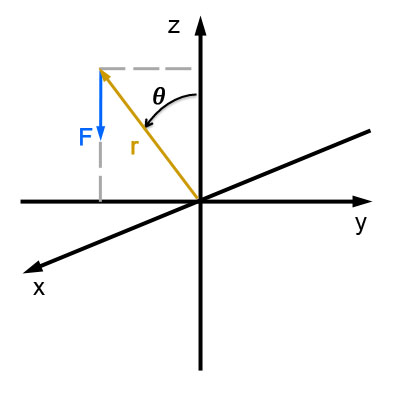
\includegraphics[width=0.4\textwidth]{ImgTorqueSol.jpg}
%  \end{center}
%\end{figure}
%\BEN
%\item Using the above coordinate system, we are given that $||\MB{r}|| = 0.14$ and $\MB{F} = -100\MB{k}$. Also, 
%\begin{align*}
%  \MB{r} &=- \sin(30^{\circ})||\MB{r}||\MB{j} + \cos(30^{\circ} )||\MB{r}||\MB{k}\\
%  &= -0.07\MB{j} + 0.07\sqrt{3}\MB{k}\\
%  &= 0.07\big(-\MB{j} + \sqrt{3}\MB{k}\big)
%\end{align*}
%To compute the torque when $\theta = 30^{\circ}$, we use the cross product:
%\begin{align*}
%0.07
%\begin{vmatrix}
%   \MB{i} & \MB{j} &  \MB{k} \\
%   0 & -1 &  \sqrt{3} \\
%   0 & 0 & -100  \\
%  \end{vmatrix}=7\MB{i}
%\end{align*} 
%Thus, the magnitude of the torque $\boldsymbol\tau$ is 7 N$\cdot$m. A similar calculation for $\theta = 90^{\circ}$ yields a magnitude of 14 N$\cdot$m
%% ~  ~  ~  ~  ~  ~  ~  ~  ~  ~  ~  ~  ~  ~  ~  ~  ~  ~  ~  ~  ~  ~  ~  ~  ~  ~  ~  
%\item Using a similar calculation from above, 
%\begin{align*}
%  \MB{r} &=- \sin\theta||\MB{r}||\MB{j} + \cos\theta||\MB{r}||\MB{k}\\
%  &= -0.14\sin\theta\MB{j} + 0.14\cos\theta\MB{k}
%\end{align*}
%To compute the torque when $\theta = 30^{\circ}$, we use the cross product:
%\begin{align*}
%0.14
%\begin{vmatrix}
%   \MB{i} & \MB{j} &  \MB{k} \\
%   0 & -\sin\theta &  \cos\theta \\
%   0 & 0 & -100  \\
%  \end{vmatrix}=14\sin\theta\MB{i}
%\end{align*} 
%Thus, the magnitude of the torque $\boldsymbol\tau$ is $|| 14\sin\theta\MB{i} || \text{N}\cdot\text{m} = 14 |\sin\theta|$N$\cdot$m.
%% ~  ~  ~  ~  ~  ~  ~  ~  ~  ~  ~  ~  ~  ~  ~  ~  ~  ~  ~  ~  ~  ~  ~  ~  ~  ~  ~  
%\item The magnitude is minimized when $\theta = 0$ or $180^{\circ}$. This corresponds to angles when $\MB{F}$ and $\MB{r}$ are parallel (or anti-parallel). The cross product of two vectors that are parallel (or anti-parallel) is zero.  
%\EEN
%
%%%%%%%%%%%%%%%%%%%%%%%%%%%%%%%%%%%%%%%
%%%%%%%%%%%%%%%%%%%%%%%%%%%%%%%%%%%%%%%
%%%%%%%%%%%%%%%%%%%%%%%%%%%%%%%%%%%%%%%
%
\EEN


\newpage % Page Break
% ~  ~  ~  ~  ~  ~  ~  ~  ~  ~  ~  ~  ~  ~  ~  ~  ~  ~  ~  ~  ~  ~  ~  ~
\subsection{Surfaces}
\rednote{We'll have solutions to 3 or 4 questions on this topic here.}
\newpage % Page Break
% ~  ~  ~  ~  ~  ~  ~  ~  ~  ~  ~  ~  ~  ~  ~  ~  ~  ~  ~  ~  ~  ~  ~  ~
\subsection{Curvilinear Coordinates}
\rednote{We'll have solutions to 3 or 4 questions on this topic here.}
\newpage % Page Break
% ~  ~  ~  ~  ~  ~  ~  ~  ~  ~  ~  ~  ~  ~  ~  ~  ~  ~  ~  ~  ~  ~  ~  ~
\subsection{Vector-Valued Functions}
%
\BEN 
%% ~~~~~~~~~~~~~~~~~~~~~~~~~~~~~~~~~~~~~~~~~~~~~~~~~~~~~~~~~~~~~~~~~~~~~~~~~~~~~~~~~
%\item 
%Use row-reduction operations on the augmented matrices.
%\begin{align}
% \begin{amatrix}{4}
%  1 & 2 & 0 & 1 & 1 \\
%  3 & -1 & 1 & 2 & 5 \\
%  0 & 1 & 0 & 2 & 0 \\
%  4 & 0 & 3 & 1 & 10
% \end{amatrix}&
% \nonumber \\
% \begin{amatrix}{4}
%  1 & 2 & 0 & 1 & 1 \\
%  0 & -7 & 1 & -1 & 2 \\
%  0 & 1 & 0 & 2 & 0 \\
%  0 & -8 & 3 & -3 & 6
% \end{amatrix}&
% \begin{array}{l}
%  R_2 \leftarrow R_2 - 3R_1 \\ R_4 \leftarrow R_4 - 4R_1 
% \end{array}
% \nonumber \\
% \begin{amatrix}{4}
%  1 & 2 & 0 & 1 & 1 \\
%  0 & 0 & 1 & 13 & 2 \\
%  0 & 1 & 0 & 2 & 0 \\
%  0 & 0 & 3 & 13 & 6
% \end{amatrix}&
% \begin{array}{l}
%  R_2 \leftarrow R_2 + 7R_3 \\ R_4 \leftarrow R_4 + 8R_3
% \end{array}
% \nonumber \\
% \begin{amatrix}{4}
%  1 & 2 & 0 & 1 & 1 \\
%  0 & 0 & 1 & 13 & 2 \\
%  0 & 1 & 0 & 2 & 0 \\
%  0 & 0 & 0 & -26 & 0
% \end{amatrix}&
% \begin{array}{l}
%  R_4 \leftarrow R_4 - 3R_2
% \end{array}
% \nonumber
%\end{align}
%
%This is equivalent to the system of equations
%
%\begin{align}
% x + 2y + w &= 1 \nonumber \\
% z + 13w &= 2 \nonumber \\
% y + 2w &= 0 \label{q2_a:a} \\
% -26w &= 0 \label{q2_a:b}
%\end{align}
%
%Equations (\ref{q2_a:a}) and (\ref{q2_a:b}) show that $w = 0$ and
%$y = 0$, and substitution yields $z = 2$ and $x = 1$.
%
%% ~~~~~~~~~~~~~~~~~~~~~~~~~~~~~~~~~~~~~~~~~~~~~~~~~~~~~~~~~~~~~~~~~~~~~~~~~~~~~~~~~
%\item
%\BEN
%\item
%It's not possible to calculate the determinant of $A$, because $A$ is not square. We can however solve $A\mathbf{x}=\mathbf{b}$ for \textbf{x} using row operations:
%\begin{align}
% \begin{amatrix}{4}
%  -3 &  1 & 2 &  4 & 1 \\
%   2 & -1 & 2 &  3 & 1 \\
%   1 &  0 & 4 & -2 & 1
% \end{amatrix}&
% \nonumber \\
% \begin{amatrix}{4}
%  0 &  1 & 14 & -2 &  4 \\
%  0 & -1 & -6 &  7 & -1 \\
%  1 &  0 &  4 & -2 &  1
% \end{amatrix}&
% \begin{array}{l}
%  R_1 \leftarrow R_1 + 3R_3 \\ R_2 \leftarrow R_2 - 2R_3
% \end{array}
% \nonumber \\
% \begin{amatrix}{4}
%  0 & 1 & 14 & -2 & 4 \\
%  0 & 0 &  8 &  5 & 3 \\
%  1 & 0 &  4 & -2 & 1
% \end{amatrix}&
% \begin{array}{l}
%  R_2 \leftarrow R_2 + R_1
% \end{array}
% \nonumber
%\end{align}
%
%This is equivalent to the system of equations
%
%\begin{align}
% y + 14z -2w &= 4 \label{asdfasdf} \\
% 8z + 5w &= 3 \label{qwerqwer} \\
% x + 4z -2w &= 1 \label{zxcvzxcv}
%\end{align}
%
%Since there are fewer equations than unknowns we will parameterize the 
%solution set by setting $w = t$, where $t$ is any real number.  From equation 
%(\ref{qwerqwer}) we get $z = \frac{3}{8} - \frac{5}{8}t$.  Substituting $z$ into 
%equations (\ref{zxcvzxcv}) and (\ref{asdfasdf}) yields $x = -\frac{1}{2} + 
%\frac{9}{2}t$ and $y = -\frac{5}{4} + \frac{43}{4}t$. \\
%
%Because of the free parameter $t$, there are infinitely many solutions to the given system.
%% ~  ~  ~  ~  ~  ~  ~  ~  ~  ~  ~  ~  ~  ~  ~  ~  ~  ~  ~  ~  ~  ~  ~  ~  ~  ~  ~  ~  ~  ~  ~  ~  ~  ~  ~  ~  
%\item
%We can calculate the 3$\times$3 determinant by expanding into 2$\times$2 determinants:
%\begin{align*}
% \begin{vmatrix}
%  1 &  2 & -1 \\
%  2 &  5 &  0 \\
% 4 & 9 &  -2
% \end{vmatrix} &=
% 1 \begin{vmatrix} 5 & 0 \\ 9 & -2 \end{vmatrix}
% -2 \begin{vmatrix} 2 & 0 \\ 4 & -2 \end{vmatrix}
% -1 \begin{vmatrix} 2 & 5 \\ 4 & 9 \end{vmatrix} \\
% &= (-10) -2 (-4) -(18 - 20) \\
% &= -10 + 8 + 2 \\
% &= 0
%\end{align*}
%Applying one row operation yields
%\begin{align*}
% \begin{amatrix}{3}
%  1 & 2 & -1  & 1 \\
%  2 & 5 & 0 & 5 \\
%  4 & 9 & -2 & 0 
% \end{amatrix} \sim
%  \begin{amatrix}{3}
%  1 & 2 & -1  & 1 \\
%  2 & 5 & 0 & 5 \\
%  0 & 0 & 0 & -7
% \end{amatrix}
%  \begin{array}{l}
%  \\ \\
%  R_3 \leftarrow R_3 - 2R_1 - R_2  \
% \end{array}
% \end{align*}
% The last row is equivalent to 
% \begin{align*}
%0x+0y+0z = -7,
%\end{align*}
%which implies that this particular system has no solution. 
% % ~~~~~~~~~~~~~~~~~~~~~~~~~~~~~~~~~~~~~~~~~~~~~~~~~~~~~~~~~~~~~~~~~~~~~~~~~~~~~~~~~
%\EEN

\item The derivative of $\textbf{r}$ is simply
\(
  \mathbf{r}'(t) = 2t \mathbf{i} + \mathbf{j}.
\)

\BEN
\item \(
  \mathbf{r}(t) \perp  \mathbf{r}'(t)
\)
implies
\begin{align*}
  0& = \mathbf{r}(t) \cdot  \mathbf{r}'(t) \\
  &= \big((1+t^2) \mathbf{i} + t\mathbf{j} \big) \cdot \big(2t \mathbf{i} + \mathbf{j}\big) \\
  &= (2t+2t^3) + (t)\\
  &= t(3+2t^2)
\end{align*}
This equation is satisfied only when $t=0$ or $t^2 = -3/2$. The latter equation cannot be satisfied if $t\in\R$. Thus, the two vectors are only perpendicular when $t=0$. Thus,  \(\mathbf{r}(t)\) is perpendicular to \(\mathbf{r}'(t)\) at (0,1). 
\item If \(\mathbf{r}(t)\) is pointing in the same direction as \(\mathbf{r}'(t)\), then \ \(\mathbf{r}(t) = C  \mathbf{r}'(t)\), where $C$ is a positive constant. Equating the components of the vectors yields the two equations
\begin{align*}
  (1+t^2)& = C2t , \text{ and } t=C.
\end{align*}
If we substitute $t=C$ into the first equation, we find
\begin{align*}
  (1+C^2)& = 2C^2\\
  C&=+1,
\end{align*}
because $C$ must be positive. Thus, the two vectors are pointing in the same direction when $t=1$, which is at the point (2,1).
\item
The solution is the similar to part (b), except that $C$ must be a negative constant. We find that the vectors point in opposite directions when $C=t=-1$, and at the point (2,-1).
\EEN
% ~~~~~~~~~~~~~~~~~~~~~~~~~~~~~~~~~~~~~~~~~~~~~~~~~~~~~~~~~~~~~~~~~~~~~~~~~~~~~~~~~

%\item
%We first convert the system of equations into an equivalent augmented-matrix
%form:
%\[
% \begin{amatrix}{3}
%  1 & 2 & -1 & 2 \\
%  2 & a & -2 & b \\
%  3 & 2 & 0 & 1
% \end{amatrix}.
%\]
%Then apply a sequence of row-reduction operations:
%\begin{align}
% \begin{amatrix}{3}
%  1 &   2 & -1 &   2 \\
%  0 & a-4 &  0 & b-4 \\
%  0 &  -4 &  3 &  -5
% \end{amatrix} &  \nonumber \\
% \begin{amatrix}{3}
%  1 &  2 & -1 &   2 \\
%  0 &  a & -3 & b+1 \\
%  0 & -4 &  3 &  -5
% \end{amatrix} & \begin{array}{l} R_2 - 2R_1 \\ R_3 - 3R_1 \end{array} 
% \nonumber \\
% \begin{amatrix}{3}
%  1 & 2 & -1 &   2 \\
%  0 & a & -3 & b+1 \\
%  0 & 4 & -3 &   5
% \end{amatrix} &  \begin{array}{l} R_2 - R_3 \end{array}
% \nonumber \\
% \begin{amatrix}{3}
%  1 & 2 & -1 &   2 \\
%  0 & 4 & -3 &   5 \\
%  0 & a & -3 & b+1
% \end{amatrix} &\begin{array}{l} -1 \cdot R_3 \\ R_2 \leftrightarrow R_3 \end{array}
% \label{eq:reduced}
%\end{align}
%
%Suppose that $a = 4$.  Then (\ref{eq:reduced}) becomes
%\begin{align}
% \begin{amatrix}{3}
%  1 & 2 & -1 &   2 \\
%  0 & 4 & -3 &   5 \\
%  0 & 4 & -3 & b+1
% \end{amatrix} &
% \nonumber \\
% \begin{amatrix}{3}
%  1 & 2 & -1 &   2 \\
%  0 & 4 & -3 &   5 \\
%  0 & 0 &  0 & b-4
% \end{amatrix}&  \begin{array}{l} R_3 - R_2 \end{array}
% \label{eq:substitute_a}
%\end{align}
%
%If $b \neq 4$, then the system has no solutions, since the last row is
%equivalent to the equation $0 = b-4$ where $b-4 \neq 0$.  Conversely, if
%$b = 4$, then (\ref{eq:substitute_a}) is equivalent to the system of
%equations
%\begin{align*}
% x + 2y -z &= 2 \\
% 4y - 3z &= 5
%\end{align*}
%There are fewer equations than unknowns, so we have to parameterize the
%solution set; let $z = t$.  Solving these two equations yields the solution
%\begin{equation}\begin{aligned}
% x &= -\frac{1}{2} - \frac{1}{2}t \\
% y &= \frac{5}{4} + \frac{3}{4}t \\
% z &= t
%\end{aligned}\label{q4:inf}\end{equation}
%
%Now suppose that $a = 0$.  Then the matrix (\ref{eq:reduced}) is equivalent
%to the system
%
%\begin{align*}
% x + 2y -z &= 2 \\
% 4y -3z &= 5 \\
% -3z &= b+1
%\end{align*}
%
%Using back-substitution we find that
%
%\begin{equation}\begin{aligned}
% x &= -\frac{1}{3} - \frac{1}{6}b \\
% y &= 1 - \frac{1}{4}b \\
% z &= \frac{-1}{3} - \frac{1}{3}b
%\end{aligned}\label{q4:a_zero}\end{equation}
%
%Now suppose that $a \neq 4$ and $a \neq 0$.  Then we can continue row-
%reducing from (\ref{eq:reduced}):
%
%\begin{align}
% \begin{amatrix}{3}
%  1 & 2 & -1 &   2 \\
%  0 & 4 & -3 &   5 \\
%  0 & a & -3 & b+1
% \end{amatrix} &
% \nonumber \\
% \begin{amatrix}{3}
%  1 & 2 & -1 & 2 \\
%  0 & 4 & -3 & 5 \\
%  0 & 0 & -3 + \frac{3}{4}a & 1 + b - \frac{5}{4}a
% \end{amatrix}&
% \begin{array}{l}
%  R_3 \leftarrow R_3 - \dfrac{a}{4}R_2
% \end{array} 
% \nonumber
%\end{align}
%
%This is equivalent to the system
%
%\begin{align*}
% x + 2y - z &= 2 \\
% 4y -3z &= 5 \\
% (-3 + \frac{3}{4}a)z &= 1 + b - \frac{5}{4}a
%\end{align*}
%
%Let $c = \dfrac{1 + b - \frac{5}{4}a}{-3 + \frac{3}{4}a}$.  Using back-substitution we find the solution
%
%\begin{equation}\begin{aligned}
% x &= -\frac{1}{2} - \frac{1}{2}c \\
% y &= \frac{5}{4} + \frac{3}{4}c \\
% z &= c
%\end{aligned}\label{q4:one}\end{equation}
%
%Thus we have shown that:
%\begin{enumerate}
%\item When $a = 4$ and $b = 4$ there are infinitely many solutions, given
%by the parameterization (\ref{q4:inf}).
%\item When $a = 4$ and $b \neq 4$ there are no solutions.
%\item When $a \neq 4$ there is one solution.  When $a = 0$, the 
%solution (\ref{q4:a_zero}) is equivalent to that of (\ref{q4:one}).  
%So the solution when $a \neq 4$ is given by (\ref{q4:one}).
%\end{enumerate}
% ~~~~~~~~~~~~~~~~~~~~~~~~~~~~~~~~~~~~~~~~~~~~~~~~~~~~~~~~~
% TORQUE, PARTICLE MOTION
\item
\BEN
\item Differentiating the equation for angular momentum yields the torque:
\begin{align*}
\mathbf{L}(t) &= m\mathbf{r}(t)\times \mathbf{r}'(t) \\
\frac{d}{dt}\mathbf{L}(t) &= \frac{d}{dt} \Big(m\mathbf{r}(t)\times \mathbf{r}'(t) \Big)\\
&=m\mathbf{r}'(t)\times \mathbf{r}'(t) + m\mathbf{r}(t)\times \mathbf{r}''(t) \\
&=m\mathbf{0}  + m\mathbf{r}(t)\times \mathbf{r}''(t) \\
&=m\mathbf{r}(t)\times \mathbf{r}''(t) \\
&= \boldsymbol\tau(t)
\end{align*}
% ~  ~  ~  ~  ~  ~  ~  ~  ~  ~  ~  ~  ~  ~  ~  ~  ~  ~  ~  ~  ~  ~  ~  ~  
\item If each component of $\mathbf{\tau}(t)$ is zero for all values of $t$, then each component of $\mathbf{L}'(t)$ is zero for all values of $t$. Each component of $\mathbf{L}(t)$ must therefore be constant. 
\EEN
% ~~~~~~~~~~~~~~~~~~~~~~~~~~~~~~~~~~~~~~~~~~~~~~~~~~~~~~~~~~~~~~~~~~~~~~~~~~~~~~~~~
%% POLYNOMIAL INTERPOLATION
%\item
%\BEN
%\item
%We can write the system as
%\begin{align*}
%a_0+a_1(0)+a_2(0)^2 +a_3(0)^3 &= 0 \\
%a_0+a_1(1)+a_2(1)^2 +a_3(1)^3 &= 5.5 \\
%a_0+a_1(2)+a_2(2)^2 +a_3(2)^3&= 20  \\
%a_0+a_1(3)+a_2(3)^2 +a_3(3)^3 &= 46.5 \\
%a_0+a_1(4)+a_2(4)^2 +a_3(4)^3 &= 88 \\ 
%\end{align*}
%Equivalently, we can write this as
%\begin{align*}
%\BM
%1 & 0 & 0 & 0 \\
%1 & 1 &1 &1\\
%1&2&4&8\\ 
%1&3&9&27\\ 
%1&4&16&64\\ 
% \EM
% \BM a_0\\a_1\\a_2\\a_3 \EM 
% =  \BM 0\\5.5\\20\\46.5\\88 \EM 
%\end{align*}
%
%\item
%Solving the above system yields 
%\begin{align*}
% \BM a_0\\a_1\\a_2\\a_3 \EM 
% =  \BM 0\\2\\3\\0.5 \EM 
%\end{align*}
%
%\item
%$p(1.5) = 2(1.5)+3(1.5)^2+0.5(1.5)^3 = 11.4375$
%
%
%\item
%The system for a polynomial of lower order would have no solution because $a_3 \ne 0$. For example, if we used a linear function, the system becomes
%\begin{align*}
%\BM
%1&0\\
%1&1\\
%1&2\\ 
%1&3\\ 
%1&4\\ 
% \EM
% \BM a_0\\a_1 \EM 
% =  \BM 0\\5.5\\20\\46.5\\88 \EM 
%\end{align*}
%This system has no solution. 
%
%\EEN
% ~~~~~~~~~~~~~~~~~~~~~~~~~~~~~~~~~~~~~~~~~~~~~~~~~~~~~~~~~
% INTEGRATION, PARTICLE MOTION
\item 
\BEN
\item 
From $\MB{F}=m\MB{a} = m\MB{v}'(t)$ we obtain
\begin{align*}
  \MB{v}(t) &= c_1\MB{i}+ \big(\pi\sin(\pi t)+c_2\big)\MB{j} + \big(- \pi \cos(\pi t) + c_3\big) \MB{k}
\end{align*}
where $c_1,c_2,c_3$ are constants. When $t=0$,  
\begin{align*}
  \MB{v}(0) &= c_1\MB{i}+ \big(\pi\sin(0)+c_2\big)\MB{j} + \big(- \pi \cos(0) + c_3\big) \MB{k}\\
  &= c_1\MB{i}+c_2\MB{j} + ( -\pi + c_3) \MB{k}
\end{align*}
But $\MB{v}(0) = \MB{i}$, so by comparison, $c_1= 1$, $c_2 = 0$, and $c_3=\pi$. Thus
\begin{align*}
  \MB{v}(t) &= \MB{i}+ \big(\pi\sin(\pi t)\big)\MB{j} + \big(- \pi \cos(\pi t) + \pi\big) \MB{k}
\end{align*}
% ~  ~  ~  ~  ~  ~  ~  ~  ~  ~  ~  ~  ~  ~  ~  ~  ~  ~  ~  ~  ~  
\item Integrating the components of $\MB{v}(t)$ yields
\begin{align*}
  \MB{r}(t) &= (t+d_1)\MB{i}+ \big(-\cos(\pi t)+d_2\big)\MB{j} + \big(- \sin(\pi t) + \pi t + d_3\big) \MB{k}
\end{align*}
where $d_1,d_2$ and $d_3$ are constants. When $t=0$,  
\begin{align*}
  \MB{r}(0) &= (0+d_1)\MB{i}+ \big(-\cos(0)+d_2\big)\MB{j} + \big(- \sin(0) + \pi (0) + d_3\big) \MB{k} \\
  \MB{r}(0) &= d_1\MB{i}+ \big(-1+d_2\big)\MB{j} + \big(d_3\big) \MB{k}
\end{align*}
But $\MB{r}(0) = -\MB{i}$, so by comparison, $d_1= -1$, $d_2 = 1$, and $d_3=0$. Thus
\begin{align*}
  \MB{r}(t) &= (t-1)\MB{i}+ \big(-\cos(\pi t)+1\big)\MB{j} + \big(- \sin(\pi t) + \pi t\big) \MB{k}
\end{align*}
Thus
\begin{align*}
  \MB{r}(1) &= (1-1)\MB{i}+ \big(-\cos(\pi)+1\big)\MB{j} + \big(- \sin(\pi) + \pi \big) \MB{k} \\
  &= 2\MB{j} + \pi\MB{k}
\end{align*}
% ~  ~  ~  ~  ~  ~  ~  ~  ~  ~  ~  ~  ~  ~  ~  ~  ~  ~  ~  ~  ~  
\item At $t=0$ and $t=1$ we have 
\begin{align*}
  \MB{r}(0) &= \BM -1 \\ 0 \\ 0 \EM , \quad
  \MB{r}(1) = \BM 0 \\ 2 \\ \pi \EM.
\end{align*}
\EEN
\begin{figure}[h]
  \vspace{-10pt}
  \begin{center}
    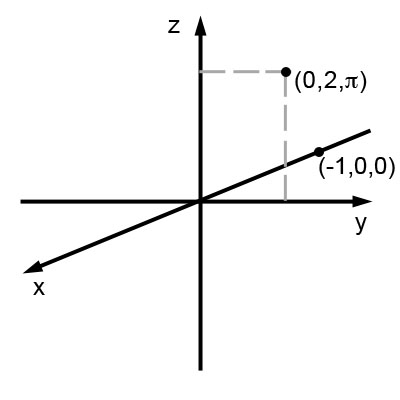
\includegraphics[width=0.45\textwidth]{ImgParticle.jpg}
  \end{center}
  \vspace{-20pt}
\end{figure}
% ~~~~~~~~~~~~~~~~~~~~~~~~~~~~~~~~~~~~~~~~~~~~~~~~~~~~~~~~~
\EEN % END OF SOLUTIONS


% ~~~~~~~~~~~~~~~~~~~~~~~~~~~~~~~~~~~~~~~~~~~~~~~~~~~~~~~~~
% ~~~~~~~~~~~~~~~~~~~~~~~~~~~~~~~~~~~~~~~~~~~~~~~~~~~~~~~~~

% QUESTIONS AND SOLUTIONS ON SIMILAR AND ORTHOGONAL MATRICES

%% -  -  -  -  -  -  -  -  -  -  -  -  -  -  -  -  -  -  -  -  -  -  -  -  -  -  -  -  -  -  
%\item 
%% QUESTION 5, MEDIUM
%%GPS: MMCA2c
%Let $A, B, C$ be three square matrices with the same dimensions.
%\begin{enumerate}
%\item Prove that if $A$ and $B$ are similar and $B$ and $C$ are similar then 
%$A$ and $C$ are similar.
%\item Let $x \in R$.  Prove that $A$ and $B + xI$ are similar whenever
%$A - xI$ and $B$ are similar.
%\item Suppose the system $A\mathbf{x} = \mathbf{b}$ has infinitely many solutions $x$ and that
%$A$ and $B$ are similar.  How many solutions can $B\mathbf{x} = \mathbf{b}$ have?
%\end{enumerate}
%
%% -  -  -  -  -  -  -  -  -  -  -  -  -  -  -  -  -  -  -  -  -  -  -  -  -  -  -  -  -  -  
%\item 
%% QUESTION 6, MEDIUM
%%GPS: MMCA2b 
%
%\begin{enumerate}
%\item Prove that, for any vectors $\mathbf{u}, \mathbf{v}$ and any orthogonal matrix $X$, $\mathbf{u} 
%\cdot \mathbf{v} = X\mathbf{u} \cdot X\mathbf{v}$
%\item Let $\mathbf{u}$ and $\mathbf{v}$ be two distinct vectors in $\R^{2}$.  Prove that, when 
%$X$ is an orthogonal matrix, the area of the parallelogram determined by $\mathbf{u}$ 
%and $\mathbf{v}$ is equal to the area of the parallelogram determined by $X\mathbf{u}$ and 
%$X\mathbf{v}$.
%\end{enumerate}

%
%\subsubsection*{(b)}
%
%Form the augmented matrix and apply row-reduction operations:
%
%\begin{align}
% \begin{bmatrix}
%  1 & 2 & -1 & 1 & 0 & 0 \\
%  2 & 5 & 0 & 0 & 1 & 0 \\
%  -3 & -5 & 4 & 0 & 0 & 1
% \end{bmatrix}&
% \nonumber \\
% \begin{bmatrix}
%  1 & 2 & -1 & 1 & 0 & 0 \\
%  0 & 1 & 2 & -2 & 1 & 0 \\
%  0 & 1 & 1 & 3 & 0 & 1
% \end{bmatrix}&
% \begin{array}{l}
%  R_2 \leftarrow R_2 - 2R_1 \\
%  R_3 \leftarrow R_3 + 3R_1
% \end{array}
% \nonumber \\
% \begin{bmatrix}
%  1 & 2 & -1 & 1 & 0 & 0 \\
%  0 & 1 & 2 & -2 & 1 & 0 \\
%  0 & 0 & -1 & 5 & -1 & 1
% \end{bmatrix}&
% \begin{array}{l}
%  R_3 \leftarrow R_3 - R_2
% \end{array}
% \nonumber \\
% \begin{bmatrix}
%  1 & 2 & -1 & 1 & 0 & 0 \\
%  0 & 1 & 0 & 8 & -1 & 2 \\
%  0 & 0 & 1 & -5 & 1 & -1
% \end{bmatrix}&
% \begin{array}{l}
%  R_2 \leftarrow R_2 + 2R_3 \\
%  R_3 \leftarrow -1 * R_3
% \end{array}
% \nonumber \\
% \begin{bmatrix}
%  1 & 0 & 0 & -20 & 3 & -5 \\
%  0 & 1 & 0 & 8 & -1 & 2 \\
%  0 & 0 & 1 & -5 & 1 & -1
% \end{bmatrix}&
% \begin{array}{l}
%  R_1 \leftarrow R_1 - 2R_2 + R_3
% \end{array}
% \nonumber
%\end{align}
%
%So the inverse matrix is
%\(\begin{bmatrix} -20 & 3 & -5 \\ 8 & -1 & 2 \\ -5 & 1 & -1 \end{bmatrix}\).
%
%\subsubsection*{(c)}
%
%The matrices $A_i$ are found by replacing the $i^{th}$ column of $A$ with
%the vector $b$.
%
%\begin{align*}
% A_1 &=
%  \begin{bmatrix}
%   1 & 2 & -1 \\
%   2 & 5 & 0 \\
%   -1 & -5 & 4
%  \end{bmatrix}, \det(A_1) = 20 - 16 + 5 = 9 \\
% A_2 &=
%  \begin{bmatrix}
%   1 & 1 & -1 \\
%   2 & 2 & 0 \\
%   -3 & -1 & 4
%  \end{bmatrix}, \det(A_2) = 8 - 8 - 4 = -4 \\
% A_3 &=
%  \begin{bmatrix}
%   1 & 2 & 1 \\
%   2 & 5 & 2 \\
%   -3 & -5 & -1
%  \end{bmatrix}, \det(A_3) = 5 - 8 + 5 = 2
%\end{align*}
%\subsection*{Question 5}
%
%\subsubsection*{(a)}
%Since $A$ and $B$ are similar and $B$ and $C$ are similar there exist
%matrices $S$ and $T$ such that $A = S^{-1}BS$ and $B = T^{-1}CT$; by
%substitution we see that $A = S^{-1}(T^{-1}CT)S = (TS)^{-1}C(TS)$.  If
%we set $U = TS$, then $A = U^{-1}CU$, so that A and C are similar.
%
%\subsubsection*{(b)}
%Since $A - xI$ and $B$ are similar there exists a square invertible matrix
%$C$ such that $C^{-1}(A - xI)C = B$.  By expanding the left-hand side of the
%equation we get $C^{-1}AC - C^{-1}xIC = B$.  However, since $x$ is a scalar,
%$C^{-1}xIC = xC^{-1}IC = xC^{-1}C = xI$, so that $C^{-1}AC - xI = B$.  By
%rearranging we see that $B + xI = C^{-1}AC$, so that $A$ and $B + xI$ are
%similar.
%
%\subsubsection*{(c)}
%Since $A$ and $B$ are similar, they have the same determinant.  The system
%$A\mathbf{x} = \mathbf{b}$ has infinitely many solutions, which, since $A$ is square, implies 
%that $A$ is not invertible, so that $\det(A) = \det(B) = 0$.  Therefore the 
%system $B\mathbf{x} = \mathbf{b}$ is either unsolvable or has infinitely many solutions.
%
%\subsection*{Question 6}
%
%\subsubsection*{(a)}
%Since $\mathbf{u} \cdot \mathbf{v} = \mathbf{u}^{T}\mathbf{v}$ for any vectors $\mathbf{u}, \mathbf{v}$ and $X^{T}X = I$, $X\mathbf{u}
%\cdot X\mathbf{v} = (X\mathbf{u})^{T}X\mathbf{v} = \mathbf{u}^{T}X^{T}X\mathbf{v} = \mathbf{u}^{T}\mathbf{v} = \mathbf{u} \cdot \mathbf{v}$.
%
%\subsubsection*{(b)}
%The area $area_{\mathbf{u},\mathbf{v}}$ of the parallelogram determined by $\mathbf{u}$ and $\mathbf{v}$ is given by the magnitude of the cross product $\mathbf{u} \times \mathbf{v}$:
%\[area_{\mathbf{u},\mathbf{v}} = ||\mathbf{u}||||\mathbf{v}|| \cdot |\sin(\theta_{\mathbf{u},\mathbf{v}})|\]
%where $\theta_{\mathbf{u},\mathbf{v}}$ is the angle between the vectors $\mathbf{u}, \mathbf{v}$.  Similarly,
%\[area_{X\mathbf{u},X\mathbf{v}}\ = ||X\mathbf{u}||||X\mathbf{v}|| \cdot |\sin(\theta_{X\mathbf{u},X\mathbf{v}})|\]
%Applying part (a) we see that $||X\mathbf{u}|| = \sqrt{X\mathbf{u} \cdot X\mathbf{u}} = \sqrt{\mathbf{u} \cdot \mathbf{u}} = ||\mathbf{u}||$ and $||X\mathbf{v}|| = ||\mathbf{v}||$.  Additionally,
%\begin{align*}
% \sin(\theta_{X\mathbf{u},X\mathbf{v}}) &= \sqrt{1 - \cos(\theta_{X\mathbf{u},X\mathbf{v}})^{2}} \\
% & = \sqrt{1 - (\dfrac{X\mathbf{u} \cdot X\mathbf{v}}{||X\mathbf{u}||||X\mathbf{v}||})^{2}} \\
% &= \sqrt{1 - (\dfrac{\mathbf{u} \cdot \mathbf{v}}{||\mathbf{u}||||\mathbf{v}||})^{2}} \\
% &= \sqrt{1 - \cos(\theta_{\mathbf{u},\mathbf{v}})^{2}} \\
% &= |\sin(\theta_{\mathbf{u},\mathbf{v}})|.
%\end{align*}
%
%Thus $area_{X\mathbf{u},X\mathbf{v}} = area_{\mathbf{u},\mathbf{v}}$.


\newpage % Page Break
% ~  ~  ~  ~  ~  ~  ~  ~  ~  ~  ~  ~  ~  ~  ~  ~  ~  ~  ~  ~  ~  ~  ~  ~
\subsection{Surfaces}
\BEN
% ~~~~~~~~~~~~~~~~~~~~~~~~~~~~~~~~~~~~~~~~~~~~~~~~~~~~~~~~~
\item \Emph{Identifying Surfaces}
\BEN
\item If $ab > 0$, then $a$ and $b$ have the same sign. If they are both positive, the surface is an elliptic paraboloid that opens upward. If $a$ and $b$ are both negative, the surface is an elliptic paraboloid that opens downward. 
\item If $ab < 0$, then $a$ and $b$ have opposite signs (i.e. - one is positive, the other is negative). The surface is a hyperbolic paraboloid.
\item If $a=b = 0$, then $z=0$, which is the equation of the $xy$-plane. 
\EEN
% ~~~~~~~~~~~~~~~~~~~~~~~~~~~~~~~~~~~~~~~~~~~~~~~~~~~~~~~~~
\item \Emph{Finding the Intersection Between Two Surfaces}\\
The sphere $x^2+y^2+z^2 =9$ and the cylinder $x^2+y^2 =4$ intersect at the values of $x$ and $y$ that are satisfied by both equations. We could find these values by substituting the equation for the cylinder into the equation for the sphere:
\begin{align*}
  9 
  &= x^2+y^2+z^2 \\
  &= 4+z^2 \\
  z&=\pm\sqrt{5}
\end{align*}
Thus, the two curves intersect at $z=\sqrt{5}$ and at $z=-\sqrt{5}$. Using the equation of the sphere, we can obtain an equation for the curves that describe the intersections.
\begin{align*}
  9 
  &= x^2+y^2+(\pm\sqrt{5})^2 \\
  &= x^2+y^2+5 \\
  4&= x^2+y^2 
\end{align*}
The intersections at $z=\pm\sqrt{5}$ are described by the circle $x^2+y^2 =4$. 
% ~~~~~~~~~~~~~~~~~~~~~~~~~~~~~~~~~~~~~~~~~~~~~~~~~~~~~~~~~
\item
\Emph{Finding the Trace of a Surface}\\
The $xy$-plane is described by the equation $z=0$. Substituting $z=0$ into the equation for the hyperbolic paraboloid gives us 
\begin{align*} 0 = \frac{x^2}{a^2} - \frac{y^2}{b^2}, \end{align*}
or simply 
\begin{align*}  y^2 = \Big(\frac{b}{a}\Big)^2x^2. \end{align*}
This equation is only satisfied by two lines: 
\begin{align*}
  y&= \frac{bx}{a}, \text{ and } y=-\frac{bx}{a}. 
\end{align*}
These two lines describe the trace of the hyperbolic parabolic in the $xy$-plane.
% ~~~~~~~~~~~~~~~~~~~~~~~~~~~~~~~~~~~~~~~~~~~~~~~~~~~~~~~~~~~~~~~~~~~~~~~~~~~~~~~
\item 
\Emph{Deriving the Equation of a Surface}\\
The distance, $d_1$, from the point $(x,y,z)$ and the point $(0,1,0)$ is given by 
\begin{align*}
  d_1 = \sqrt{x^2 + (y-1)^2 + z^2}.
\end{align*}
The distance, $d_2$, from the point $(x,y,z)$ and the given plane is  
\begin{align*}
  d_2 = \big| z - 1 \big|.
\end{align*}
The points that are equidistant from the point $(0,1,0)$ and the given plane are the points that such that $d_1 = d_2$. Therefore, 
\begin{align*}
  d_1 &= d_2 \\
   \sqrt{x^2 + (y-1)^2 + z^2} &=  \big| z - 1 \big| \\
   x^2 + (y-1)^2 + z^2 &=  ( z - 1)^2 \\   
   x^2 + (y-1)^2 + z^2 &=  z^2 - 2z + 1 \\   
   x^2 + (y-1)^2  &= - 2z + 1 \\   
   z&=- \frac{1}{2} \Big(x^2 + (y-1)^2 - 1\Big)  \\   
\end{align*}
The surface is an elliptic paraboloid that opens downward and whose vertex is located at the point $(0,1,1/2)$. 

\EEN

\newpage % Page Break

\section{Partial Derivatives}

\subsection{Partial Derivatives}

\BEN

% ~~~~~~~~~~~~~~~~~~~~~~~~~~~~~~~~~~~~~~~~~~~~~~~~~~~~~~~~~
\item
\begin{enumerate}

 \item
  \begin{align*}
   \frac{\partial f}{\partial x}
   &= \frac{\partial}{\partial x}(xy \sin(\frac{x}{y})) \\
   &= y\sin(\frac{x}{y}) + xy\cos(\frac{x}{y})\frac{1}{y} \\
   &= y\sin(\frac{x}{y}) + x\cos(\frac{x}{y}) \\
   \frac{\partial^2 f}{\partial x^2}
   &= \frac{\partial}{\partial x}\frac{\partial f}{\partial x} \\
   &= \frac{\partial}{\partial x}(y\sin(\frac{x}{y}) + x\cos(\frac{x}{y})) \\
   &= y\cos(\frac{x}{y})\frac{1}{y} + \cos(\frac{x}{y}) - x\sin(\frac{x}{y})\frac{1}{y} \\
   &= 2\cos(\frac{x}{y}) - \frac{x}{y}\sin(\frac{x}{y}) \\
  \frac{\partial^2 f}{\partial y \partial x}
   &= \frac{\partial}{\partial y}\frac{\partial f}{\partial x} \\
   &= \frac{\partial}{\partial y}(y\sin(\frac{x}{y}) + x\cos(\frac{x}{y})) \\
   &= \sin(\frac{x}{y}) + y\cos(\frac{x}{y})(\frac{-x}{y^2}) - x\sin(\frac{x}{y})(\frac{-x}{y^2}) \\
   &= \sin(\frac{x}{y}) - \frac{x}{y}\cos(\frac{x}{y}) + \frac{x^2}{y^2}\sin(\frac{x}{y}) \\
   &= \frac{x^2+y^2}{y^2}\sin(\frac{x}{y}) - \frac{x}{y}\cos(\frac{x}{y}) \\
   \frac{\partial f}{\partial y}
   &= \frac{\partial}{\partial y}(xy \sin(\frac{x}{y})) \\
   &= x\sin(\frac{x}{y}) + xy\cos(\frac{x}{y})(\frac{-x}{y^2}) \\
   &= x\sin(\frac{x}{y}) - \frac{x^2}{y}\cos(\frac{x}{y}) \\
   \frac{\partial^2 f}{\partial x \partial y}
   &= \frac{\partial}{\partial x}\frac{\partial f}{\partial y} \\
   &= \frac{\partial}{\partial x}(x\sin(\frac{x}{y}) - \frac{x^2}{y}\cos(\frac{x}{y})) \\
   &= \sin(\frac{x}{y}) + x\cos(\frac{x}{y})(\frac{1}{y}) - \frac{2x}{y}\cos(\frac{x}{y}) + \frac{x^2}{y}\sin(\frac{x}{y})(\frac{1}{y}) \\
   &= \frac{x^2+y^2}{y^2}\sin(\frac{x}{y}) - \frac{x}{y}\cos(\frac{x}{y}) \\
   \nabla f
   &= \begin{bmatrix}
       \frac{\partial f}{\partial x} \\
       \frac{\partial f}{\partial y}
      \end{bmatrix} \\
   &= \begin{bmatrix}
       y\sin(\frac{x}{y}) + x\cos(\frac{x}{y}) \\
       x\sin(\frac{x}{y}) - \frac{x^2}{y}\cos(\frac{x}{y})
      \end{bmatrix}
  \end{align*}

 \item
  \begin{align*}
   \frac{\partial f}{\partial x}
   &= \frac{\partial}{\partial x}(\frac{x+y}{e^{xy}}) \\
   &= \frac{e^{xy} - (x+y)ye^{xy}}{e^{2xy}} \\
   &= \frac{1 - xy - y^2}{e^{xy}} \\
   \frac{\partial^2 f}{\partial x^2}
   &= \frac{\partial}{\partial x}\frac{\partial f}{\partial x} \\
   &= \frac{\partial}{\partial x}(\frac{1 - xy - y^2}{e^{xy}}) \\
   &= \frac{e^{xy}(-y) - (1 - xy - y^2)ye^{xy}}{e^{2xy}} \\
   &= \frac{-2y + xy^2 + y^3}{e^{xy}} \\
   \frac{\partial^2 f}{\partial y \partial x}
   &= \frac{\partial}{\partial y}\frac{\partial f}{\partial x} \\
   &= \frac{\partial}{\partial y}(\frac{1 - xy - y^2}{e^{xy}}) \\
   &= \frac{e^{xy}(-x - 2y) - (1 - xy - y^2)xe^{xy}}{e^{2xy}} \\
   &= \frac{-2x - 2y + x^2y + xy^2}{e^{xy}} \\
   \frac{\partial f}{\partial y}
   &= \frac{\partial}{\partial y}(\frac{x+y}{e^{xy}}) \\
   &= \frac{e^{xy} - (x+y)xe^{xy}}{e^{2xy}} \\
   &= \frac{1 - x^2 - xy}{e^{xy}} \\
   \frac{\partial^2 f}{\partial y^2}
   &= \frac{\partial}{\partial y}\frac{\partial f}{\partial y} \\
   &= \frac{\partial}{\partial y}(\frac{1 - x^2 - xy}{e^{xy}}) \\
   &= \frac{e^{xy}(-x) - (1 - x^2 - xy)xe^{xy}}{e^{2xy}} \\
   &= \frac{-2x + x^3 + x^2y}{e^{xy}} \\
   \frac{\partial^2 f}{\partial x \partial y}
   &= \frac{\partial}{\partial x}\frac{\partial f}{\partial y} \\
   &= \frac{\partial}{\partial x}(\frac{1 - x^2 - xy}{e^{xy}}) \\
   &= \frac{e^{xy}(-2x - y) - (1 - x^2 - xy)ye^{xy}}{e^{2xy}} \\
   &= \frac{-2x - 2y + x^2y + xy^2}{e^{xy}} \\
   \nabla f
   &= \begin{bmatrix}
       \frac{\partial f}{\partial x} \\
       \frac{\partial f}{\partial y}
      \end{bmatrix} \\
   &= \begin{bmatrix}
       \dfrac{1 - xy - y^2}{e^{xy}} \\
       \dfrac{1 - x^2 - xy}{e^{xy}}
      \end{bmatrix}
  \end{align*}

\end{enumerate}

% ~~~~~~~~~~~~~~~~~~~~~~~~~~~~~~~~~~~~~~~~~~~~~~~~~~~~~~~~~
\item

We must first compute the partial derivatives $\frac{\partial z}{\partial x}$ and $\frac{\partial z}{\partial y}$:

 \begin{align*}
  \frac{\partial}{\partial x}(xy) &= \frac{\partial}{\partial x}(z^{x+y}) \\
  y &= \frac{\partial}{\partial x}(e^{\ln(z)(x+y)}) \\
  y &= e^{\ln(z)(x+y)}\frac{\partial}{\partial x}(\ln(z)(x+y)) \\
  y &= e^{\ln(z)(x+y)}(\frac{1}{z}\frac{\partial z}{\partial x}(x+y) + \ln(z)) \\
  y &= z^{x+y}(\frac{x+y}{z}\frac{\partial z}{\partial x} + \ln(z)) \\
  y &= \frac{\partial z}{\partial x}(x+y)z^{x+y-1} + z^{x+y}\ln(z) \\
  \frac{\partial z}{\partial x} &= \frac{y - z^{x+y}\ln(z)}{(x+y)z^{x+y-1}}
 \end{align*}

 \begin{align*}
  \frac{\partial}{\partial y}(xy) &= \frac{\partial}{\partial y}(z^{x+y}) \\
  x &= \frac{\partial}{\partial y}(e^{\ln(z)(x+y)}) \\
  x &= e^{\ln(z)(x+y)}\frac{\partial}{\partial y}(\ln(z)(x+y)) \\
  x &= e^{\ln(z)(x+y)}(\frac{1}{z}\frac{\partial z}{\partial y}(x+y) + \ln(z)) \\
  x &= z^{x+y}(\frac{x+y}{z}\frac{\partial z}{\partial y} + \ln(z)) \\
  x &= \frac{\partial z}{\partial y}(x+y)z^{x+y-1} + z^{x+y}\ln(z) \\
  \frac{\partial z}{\partial y} &= \frac{x - z^{x+y}\ln(z)}{(x+y)z^{x+y-1}}
 \end{align*}

So $\nabla h(x,y) = \begin{bmatrix}
                \dfrac{y - z^{x+y}\ln(z)}{(x+y)z^{x+y-1}} \\
                \dfrac{x - z^{x+y}\ln(z)}{(x+y)z^{x+y-1}}
               \end{bmatrix}$.

% ~~~~~~~~~~~~~~~~~~~~~~~~~~~~~~~~~~~~~~~~~~~~~~~~~~~~~~~~~
\item

 Recall that the equation of the plane tangent to the surface defined by
 $g(x,y,z) = 0$ at the point $(x_0, y_0, z_0)$ is $\nabla g(x_0,y_0,z_0)
 \cdot \begin{bmatrix} x - x_0 \\ y - y_0 \\ z - z_0 \end{bmatrix} = 0$.

 \begin{enumerate}
  \item Define $g(x,y,z) = f(x,y) - z = \frac{x^2}{9} - y^2 - z$, so that the
   surface  $z = f(x,y)$ is equivalently defined by the equation
   $g(x,y,z) = 0$.
   We can then find the equation of the tangent plane at the point
   $(2, \frac{1}{3}, \frac{1}{3})$ by computing $\nabla g$ and applying the
   above formula:

   \begin{align*}
    \nabla g(x,y,z) &=
     \begin{bmatrix} \frac{2x}{9} \\ -2y \\ -1 \end{bmatrix} \\
    \nabla g(2,\frac{1}{3},\frac{1}{3}) &=
     \begin{bmatrix} \frac{4}{9} \\ -\frac{2}{3} \\ -1 \end{bmatrix} \\
   \end{align*}

   This yields the equation
   \begin{align*}
    \frac{4}{9}(x - 2) - \frac{2}{3}(y - \frac{1}{3}) - (z - \frac{1}{3}) &= 0 \\
    \frac{4}{9}x - \frac{2}{3}y - z &= \frac{1}{3} \\
    4x - 6y - 9z &= 3.
   \end{align*}

  \item Define $g(x,y,z) = x^2 + x + y - z^2 - 7$.  Then compute
   \begin{align*}
    \nabla g(x,y,z) &= \begin{bmatrix} 2x + 1 \\ 1 \\ -2z \end{bmatrix} \\
    \nabla g(2,5,2) &= \begin{bmatrix} 5 \\ 1 \\ -4 \end{bmatrix}.
   \end{align*}

   Thus the equation of the tangent plane is
   \begin{align*}
    5(x - 2) + (y - 5) - 4(z - 2) &= 0 \\
    5x + y - 4z &= 7.
   \end{align*}
 \end{enumerate}

% ~~~~~~~~~~~~~~~~~~~~~~~~~~~~~~~~~~~~~~~~~~~~~~~~~~~~~~~~~
\item

 \begin{enumerate}
  \item $f$ will increase fastest in the direction of the vector
   $\nabla f(x_0,y_0)$ from the point $(x_0, y_0)$.  Therefore we compute and
   evaluate the gradient $\nabla f$ at the point $(1, 1)$:

   \begin{align*}
    \nabla f &= \begin{bmatrix}
                 \dfrac{\partial f}{\partial x} \\
                 \dfrac{\partial f}{\partial y}
                \end{bmatrix} \\
             &= \begin{bmatrix}
                 \dfrac{\partial}{\partial x}(e^{-(x^2+x+1+y^2-2y)}) \\
                 \dfrac{\partial}{\partial y}(e^{-(x^2+x+1+y^2-2y)})
                \end{bmatrix} \tag{1} \label{fastest_incr:grad}  \\
             &= \begin{bmatrix}
                 (-2x - 1)e^{-(x^2+x+1+y^2-2y)} \\
                 (2y - 2)e^{-(x^2+x+1+y^2-2y)}
                \end{bmatrix} \\
    \nabla f(1, 1) &= \begin{bmatrix} -3e^{-2} \\ 0 \end{bmatrix}
   \end{align*}

 \item The rate of change of $f$ in the direction of the vector $\mathbf{v}$
  from the point $(x, y)$ is given by $\nabla f(x,y) \cdot \mathbf{v}$.  Using
  (\ref{fastest_incr:grad}) we find that $\nabla f(2, 1) =
  \begin{bmatrix} -5e^{-6} \\ 0 \end{bmatrix}$.  The direction from $(2, 1)$
  to $(5, 4)$ is given by the vector $\begin{bmatrix} 3 \\ 3 \end{bmatrix}$;
  thus the rate of change of $f$ from $(2, 1)$ towards $(5, 4)$ is
  $\begin{bmatrix} -5e^{-6} \\ 0 \end{bmatrix} \cdot
   \begin{bmatrix} 3 \\ 3 \end{bmatrix} = -15e^{-6}$.

 \end{enumerate}

% ~~~~~~~~~~~~~~~~~~~~~~~~~~~~~~~~~~~~~~~~~~~~~~~~~~~~~~~~~
\item

First we find the partial derivatives of each component with respect to each
variable:

 \begin{align*}
  \frac{\partial f_1}{\partial x} &= cos(x + y) \\
  \frac{\partial f_1}{\partial y} &= cox(x + y) \\
  \frac{\partial f_2}{\partial x} &= \frac{1}{x} \\
  \frac{\partial f_2}{\partial y} &= \frac{1}{y}
 \end{align*}

The Jacobian matrix, then, is
$\begin{bmatrix}
 cos(x + y) & cos(x + y) \\ \frac{1}{x} & \frac{1}{y}
\end{bmatrix}$.

% ~~~~~~~~~~~~~~~~~~~~~~~~~~~~~~~~~~~~~~~~~~~~~~~~~~~~~~~~~
\item

We only need to verify that (\ref{eqn:heat}) holds for the given function $u$:

\begin{align*}
 \frac{\partial u}{\partial t} &= \frac{K_0}{c\rho} \frac{\partial^2 u}{\partial x^2} \\
 -\frac{K_0}{c\rho}e^{-tK_0/(c\rho)}\sin(x) &=
 \frac{K_0}{c\rho}\frac{\partial}{\partial x}(e^{-tK_0/(c\rho)}\cos(x)) \\
 -\frac{K_0}{c\rho}e^{-tK_0/(c\rho)}\sin(x) &=
 -\frac{K_0}{c\rho}e^{-tK_0/(c\rho)}\sin(x)
\end{align*}

which is true.  So $u(x,t) = e^{-tK_0/(c\rho)}\sin(x)$ is indeed a solution
to the heat equation (\ref{eqn:heat}).

\EEN % END OF SOLUTIONS

\newpage

\subsection{Optimization}

\BEN


% ~~~~~~~~~~~~~~~~~~~~~~~~~~~~~~~~~~~~~~~~~~~~~~~~~~~~~~~~~
\item

Local extreme values of a function occur at points where the gradient of
the function is the zero vector.

 \begin{enumerate}
  \item First we find the critical points:
   \begin{align*}
    \nabla f(x,y) &= \begin{bmatrix} 0 \\ 0 \end{bmatrix} \\
    \begin{bmatrix}
     \dfrac{\partial}{\partial x}(x^2 + 2x - xy + y^2) \\
     \dfrac{\partial}{\partial y}(x^2 + 2x - xy + y^2)
    \end{bmatrix} &= \begin{bmatrix} 0 \\ 0 \end{bmatrix} \\
    \begin{bmatrix}
     2x + 2 \\
     -x + 2y
    \end{bmatrix} &= \begin{bmatrix} 0 \\ 0 \end{bmatrix} \\
    x &= -1 \\
    y &= -\frac{1}{2}
   \end{align*}
   To categorize this point $(-1, -\frac{1}{2})$ as a local minimum or maximum
   we apply the second partial derivative test:
   \begin{align*}
    D(x,y)
    &= \begin{vmatrix}
     \dfrac{\partial^2 f(x,y)}{\partial x^2} &
      \dfrac{\partial^2 f(x,y)}{\partial y \partial x} \\
     \dfrac{\partial^2 f(x,y)}{\partial x \partial y} &
      \dfrac{\partial^2 f(x,y)}{\partial y^2}
    \end{vmatrix} \\
    &= \begin{vmatrix}
     \dfrac{\partial^2}{\partial x^2}(x^2 + 2x - xy + y^2) &
      \dfrac{\partial^2}{\partial y \partial x}(x^2 + 2x - xy + y^2) \\
     \dfrac{\partial^2}{\partial x \partial y}(x^2 + 2x - xy + y^2) &
      \dfrac{\partial^2}{\partial y^2}(x^2 + 2x - xy + y^2)
    \end{vmatrix} \\
    &= \begin{vmatrix} 2 & 0 \\ -1 & 2 \end{vmatrix} \\
    &= 4 \\
    &> 0
   \end{align*}
  for all values of $x,y$.
  Additionally, $\dfrac{\partial^2 f(x,y)}{\partial x^2} = 2 > 0$, so that
  the point $(-1, -\frac{1}{2})$ is a local minimum.

  \item Again, we look for the critical points by setting the gradient to zero.
   \begin{align*}
    \nabla h(x,y) &= \begin{bmatrix} 0 \\ 0 \end{bmatrix} \\
    \begin{bmatrix} y\cos(xy) \\ x\cos(xy) \end{bmatrix}
    &= \begin{bmatrix} 0 \\ 0 \end{bmatrix}
   \end{align*}
  The solutions (and therefore the critical points) are the point $(0, 0)$
  and the family of curves $xy = \pi/2 + k\pi$, where $k \in \mathbb{Z}$.

  To categorize the points, again compute the matrix
  \begin{align*}
   D(x,y)
    &= \begin{vmatrix}
     \dfrac{\partial^2 h(x,y)}{\partial x^2} &
      \dfrac{\partial^2 h(x,y)}{\partial y \partial x} \\
     \dfrac{\partial^2 h(x,y)}{\partial x \partial y} &
      \dfrac{\partial^2 h(x,y)}{\partial y^2}
    \end{vmatrix} \\
    &= \begin{vmatrix}
     \dfrac{\partial^2}{\partial x^2}(\sin(xy)) &
      \dfrac{\partial^2}{\partial y \partial x}(\sin(xy)) \\
     \dfrac{\partial^2}{\partial x \partial y}(\sin(xy)) &
      \dfrac{\partial^2}{\partial y^2}(\sin(xy))
    \end{vmatrix} \\
    &= \begin{vmatrix}
     -y^2\sin(xy) & \cos(xy) - xy\sin(xy) \\
     \cos(xy) - xy\sin(xy) & -x^2\sin(xy)
    \end{vmatrix} \\
    D(0,0) &= \begin{vmatrix} 0 & 1 \\ 1 & 0 \end{vmatrix} \\
           &= -1 \\
   \end{align*}

   So $(0, 0)$ is a saddle point.

   \begin{align*}
    D(x, \frac{\pi/2 + k\pi}{x})
    &= \begin{vmatrix}
     -\dfrac{\pi/2 + k\pi}{x}^2\sin(\pi/2 + k\pi)
     & \cos(\pi/2 + k\pi) - (\pi/2 + k\pi)\sin(\pi/2 + k\pi) \\
     \cos(\pi/2 + k\pi) - (\pi/2 + k\pi)\sin(\pi/2 + k\pi)
     & -x^2\sin(\pi/2 + k\pi)
    \end{vmatrix} \\
    &= \begin{vmatrix}
     -(\dfrac{\pi/2 + k\pi}{x})^2 (-1)^k & - (\pi/2 + k\pi)(-1)^k \\
     - (\pi/2 + k\pi)(-1)^k & -x^2 (-1)^k
    \end{vmatrix} \\
    &= (\pi/2 + k\pi)^2 - (\pi/2 + k\pi)^2 \\
    &= 0
  \end{align*}

  So the test is inconclusive.

 \end{enumerate}

% ~~~~~~~~~~~~~~~~~~~~~~~~~~~~~~~~~~~~~~~~~~~~~~~~~~~~~~~~~
\item

We use the method of Lagrange Multipliers.  To find the extreme values
of the function $f(x,y)$ subject to the constraint $g(x,y)=c$, we define
a new function $F(x,y,t) = f(x,y) + t(g(x,y) - c)$ and solve the equation
$\nabla F(x,y,t) = 0$.  The solutions $(x,y)$ are the candidate solutions,
which we test by plugging into the original equation $f$.

\begin{enumerate}
 \item
  Define $F(x,y,t) = e^{-(x^2+y^2)} - t(x - y^2)$.  Then
  \begin{align}
   \nabla F(x,y,t) &= \begin{bmatrix} 0 \\ 0 \\ 0 \end{bmatrix} \nonumber \\
   \begin{bmatrix}
    -2xe^{-(x^2+y^2)} - t \\
    -2ye^{-(x^2+y^2)} + 2yt \\
    -(x - y^2)
   \end{bmatrix} &= \begin{bmatrix} 0 \\ 0 \\ 0 \end{bmatrix}. \label{lagr:2}
  \end{align}
  $(0,0)$ is one solution.  When $x \neq 0$, by the third component of
  (\ref{lagr:2}) we see that $y \neq 0$, so that we get $t = e^{-(x^2+y^2)}$
  from the second component, which in turn by the first component shows
  that $x = -1/2$.  However, there is no $y$ that satisfies the third
  component of (\ref{lagr:2}) when $x = -1/2$.  Thus $(0, 0)$ is the only
  extreme value.

 \item
  Define $F(x,y,t) = e^{x-y^2} - t(\frac{x^2}{4}+y+y^2 - 1)$.  Then
  \begin{align}
   \nabla F(x,y,t) &= \begin{bmatrix} 0 \\ 0 \\ 0 \end{bmatrix} \nonumber \\
   \begin{bmatrix}
    e^{x-y^2} - tx/2 \\
    -2ye^{x-y^2} - t + 2yt \\
    -(\frac{x^2}{4}+y+y^2 - 1)
   \end{bmatrix} &= \begin{bmatrix} 0 \\ 0 \\ 0 \end{bmatrix}. \label{lagr:1}
  \end{align}
  From the first two components we see that
  \begin{align*}
   e^{x-y^2} &= tx/2 \\
   e^{x - y^2} &= \frac{t-2yt}{-2y}.
  \end{align*}
  This yields the equation $y = \dfrac{1}{2-x}$, so that the extreme values
  of $f$ fall on the intersection of the ellipse $\frac{x^2}{4}+y+y^2 = 1$
  and the curve $y = \dfrac{1}{2-x}$.
  Plugging $y$ into the third component of (\ref{lagr:1}) gives the equation
  $\frac{x^2}{4} + \frac{1}{2-x} + (\frac{1}{2-x})^2 = 1$.

\end{enumerate}

% ~~~~~~~~~~~~~~~~~~~~~~~~~~~~~~~~~~~~~~~~~~~~~~~~~~~~~~~~~
\item

The divergence is given by the equation \[
 \nabla \cdot f = \frac{\partial f_1}{\partial x} + \frac{\partial f_2}{\partial y} + \frac{\partial f_3}{\partial z}
\] and the curl by the equation \[
 \nabla \times f = \begin{bmatrix}
  \dfrac{\partial f_3}{\partial y} - \dfrac{\partial f_2}{\partial z} \\
  \dfrac{\partial f_1}{\partial z} - \dfrac{\partial f_3}{\partial x} \\
  \dfrac{\partial f_2}{\partial x} - \dfrac{\partial f_1}{\partial y}
 \end{bmatrix}.
\]  Applying these equations yields the solutions:

\begin{align*}
 \nabla \cdot f &= \frac{\partial f_1}{\partial x} + \frac{\partial f_2}{\partial y} + \frac{\partial f_3}{\partial z} \\
 &= \frac{\partial}{\partial x}(x^2+y^2) + \frac{\partial}{\partial y}(y^2+z^2) + \frac{\partial}{\partial z}(z^2+x^2) \\
 &= 2x + 2y + 2z \\
 \nabla \times f &= \begin{bmatrix}
  \dfrac{\partial f_3}{\partial y} - \dfrac{\partial f_2}{\partial z} \\
  \dfrac{\partial f_1}{\partial z} - \dfrac{\partial f_3}{\partial x} \\
  \dfrac{\partial f_2}{\partial x} - \dfrac{\partial f_1}{\partial y}
 \end{bmatrix} \\
 &= \begin{bmatrix} - 2z \\ - 2x \\ - 2y \end{bmatrix}.
\end{align*}


% ~~~~~~~~~~~~~~~~~~~~~~~~~~~~~~~~~~~~~~~~~~~~~~~~~~~~~~~~~
\item

It is possible to solve this problem using Lagrangian optimization;
however, the closest point on the sphere to the plane will occur at
the point on the sphere where its normal vector is parallel to the plane's
normal vector.

% Should include more explanation for this?  Maybe not a proof,
% but perhaps a picture...

Knowing this, we first find the sphere's normal vector by computing
the gradient of the function $F(x,y,z) = x^2 + y^2 + z^2 - 1$, which by
a straightforward calculation is the vector
$\nabla F = \begin{bmatrix} 2x \\ 2y \\ 2z \end{bmatrix}$.  Now, by
rearranging the equation $x + 2y + 2z = 5$ into the form
$\begin{bmatrix} x - 3 \\ y -2 \\ z + 1 \end{bmatrix} \cdot
 \begin{bmatrix} 1 \\ 2 \\ 2 \end{bmatrix} = 0$, we see that
$\begin{bmatrix} 1 \\ 2 \\ 2 \end{bmatrix}$ is a vector normal to the plane.

We want to find a point on the sphere where these two normal vectors are
parallel; equivalently, we want to find a point on the sphere such that
$\begin{bmatrix} 2x \\ 2y \\ 2z \end{bmatrix}
 = k\begin{bmatrix} 1 \\ 2 \\ 2 \end{bmatrix}$ for some $k$.  We can plug
$x = k/2$, $y = k$, $z = k$ into the equation $x^2 + y^2 + z^2 = 1$, which
yields the solution $k = 2/3$.  Thus $(1/3, 2/3, 2/3)$ is a point on the
sphere where the sphere's normal vector is parallel to the plane's, and
therefore is the point closest to the plane.

% ~~~~~~~~~~~~~~~~~~~~~~~~~~~~~~~~~~~~~~~~~~~~~~~~~~~~~~~~~
\item

Let $l$ be the length
of the rectangular sides of the prism and $w$ be their width, so that
the sides of the equilateral triangle ends are also of length $w$.
The surface area of such a prism is given by the function $A(l,w) =
\frac{\sqrt{3}}{2}l^2 + 3lw$, and its volume by the function $V(l,w) =
\frac{\sqrt{3}}{4}l^2w$.  Since the sides cost $\$10/ft^2$ and the ends
cost $\$8/ft^2$, we wish to maximize the function $V(l,w)$ subject to
the restriction $C(l,w) = 5\sqrt{3}l^2 + 24lw = 500$.

We apply the method of Lagrange Multipliers.  Define the function
$F(l,w) = V(l,w) + t(C(l,w) - 500) =
\frac{\sqrt{3}}{4}l^2w + t(5\sqrt{3}l^2 + 24lw - 500)$;
the constrained extreme values of $V$ satisfy the equation
$\nabla F(l,w) = \mathbf{0}$.

\begin{align}
 \nabla F(l,w) &= \begin{bmatrix} 0 \\ 0 \\ 0 \end{bmatrix} \nonumber \\
 \begin{bmatrix}
  \dfrac{\partial F}{\partial l} \\
  \dfrac{\partial F}{\partial w} \\
  \dfrac{\partial F}{\partial t}
 \end{bmatrix} &= \begin{bmatrix} 0 \\ 0 \\ 0 \end{bmatrix} \nonumber \\
 \begin{bmatrix}
  \frac{\sqrt{3}}{2}lw + 10\sqrt{3}lt + 24wt \\
  \frac{\sqrt{3}}{4}l^2 + 24lt \\
  5\sqrt{3}l^2 + 24lw - 500
 \end{bmatrix} &= \begin{bmatrix} 0 \\ 0 \\ 0 \end{bmatrix} \label{soln:opt_box}
\end{align}

From the second row of (\ref{soln:opt_box}) we get $t = \frac{-\sqrt{3}}{96}l$.
Substitution into the first row yields
\begin{align}
 \frac{\sqrt{3}}{2}lw - \frac{10}{32}l^2 - \frac{\sqrt{3}}{4}lw &= 0 \nonumber \\
 \frac{\sqrt{3}}{4}lw - \frac{10}{32}l^2 &= 0 \nonumber \\
 8\sqrt{3}lw - 10l^2 &= 0 \nonumber \\
 8\sqrt{3}lw &= 10l^2 \nonumber \\
 w &= \frac{5}{4\sqrt{3}}l \label{soln:opt_box2}
\end{align}

Substituting (\ref{soln:opt_box2}) into the third row of (\ref{soln:opt_box})
yields
\begin{align*}
 5\sqrt{3}l^2 + 24l(\frac{5}{4\sqrt{3}}l) &= 500 \\
 5\sqrt{3}l^2 + \frac{30}{\sqrt{3}}l^2 &= 500 \\
 15l^2 + 30l^2 &= 500\sqrt{3} \\
 45l^2 &= 500\sqrt{3} \\
 l^2 &= \frac{100}{3^{3/2}} \\
 l &= \frac{10}{3^{3/4}}
\end{align*}

which, when combined with (\ref{soln:opt_box2}), gives
$w = \dfrac{50}{4\cdot3^{5/4}}$.

% ~~~~~~~~~~~~~~~~~~~~~~~~~~~~~~~~~~~~~~~~~~~~~~~~~~~~~~~~~
\item

We want to optimize the function $T(x,y,z) = 200xyz^2$ subject to the
constraint $x^2+y^2+z^2 = 1$.  Define the function
$F(x,y,z) = 200xyz^2 + t(x^2+y^2+z^2-1)$; the extreme points satisfy the
equation $\nabla F(x,y,z) = 0$.

\begin{align}
 \nabla F(x,y,z) &= \begin{bmatrix} 0 \\ 0 \\ 0 \\ 0 \end{bmatrix} \nonumber \\
 \begin{bmatrix}
  \dfrac{\partial F}{\partial x} \\
  \dfrac{\partial F}{\partial y} \\
  \dfrac{\partial F}{\partial z} \\
  \dfrac{\partial F}{\partial t}
 \end{bmatrix} &= \begin{bmatrix} 0 \\ 0 \\ 0 \\ 0 \end{bmatrix} \nonumber \\
 \begin{bmatrix}
  200yz^2 + 2xt \\
  200xz^2 + 2yt \\
  400xyz + 2zt \\
  x^2 + y^2 + z^2 - 1
 \end{bmatrix} &= \begin{bmatrix} 0 \\ 0 \\ 0 \end{bmatrix} \label{soln:opt_heat}
\end{align}

The third equation of (\ref{soln:opt_heat}) yields $t = -200xy$.  Substituting
this value of $t$ into the first and second equations gives $z^2 = 2x^2 = 2y^2$.
Combining this with the fourth equation yields $4x^2 = 1$, or
$x = \pm \frac{1}{2} \implies y = \pm \frac{1}{2}, z = \pm \frac{1}{\sqrt{2}}$.



\EEN

\newpage

\section{Multiple Integrals}
%
\subsection{Double Integrals}

\BEN 
% ~~~~~~~~~~~~~~~~~~~~~~~~~~~~~~~~~~~~~~~~~~~~~~~~~~~~~~~~~~~~~~~~~~~~~~~~~~~~~~~~~
\item % VOLUME OF SIMPLE SOLID 
\BEN
\item A sketch of the volume is below. 
\begin{figure}[h]
  \vspace{-1pt}
  \begin{center}
    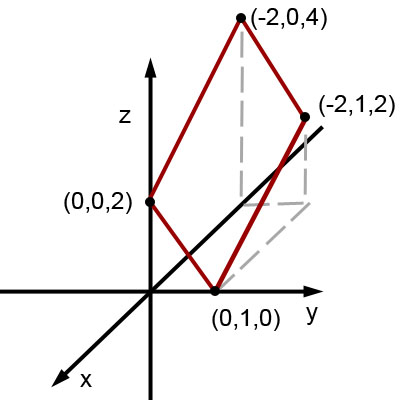
\includegraphics[width=0.35\textwidth]{ImgSolid.jpg}
  \end{center}
\end{figure}
\item We must integrate:
\begin{align*}
  \mathop{\int_{-2}^0 \! \int_0^1} (-x-2y+2 ) dydx 
  &= \int_{-2}^0 \big( -2xy -y^2 + 2y \big) \big|_0^1 dx \\
  &= \int_{-2}^0 \Big( -2x + 1  \Big) dx \\
  &= \Big(-x^2 + x \Big) \Big|_{-2}^0  \\  
  &= 0- \big(- (-2)^2 + (-2)\big)\\
  &= 0- \big(- 4 -2\big)\\
  &= 6
\end{align*}
\EEN
% ~~~~~~~~~~~~~~~~~~~~~~~~~~~~~~~~~~~~~~~~~~~~~~~~~~~~~~~~~~~~~~~~~~~~~~~~~~~~~~~~~
\item % FLUID MECHANICS
\BEN
\item Substituting the expression for $u$ into the divergence equation yields
\begin{align*}
  0&= \nabla \cdot \MB{v} \\
  &= \px \big(u(x,y)\big) + \py \big(v(x,y)\big) \\
  &= \px (x^2 + y^2) + \frac{\partial v}{\partial y}\\
  &= 2x + \frac{\partial v}{\partial y} \\
   \frac{\partial v}{\partial y} &= -2x 
\end{align*}
Therefore, $v(x,y)$ is a function whose partial derivative with respect to $y$ is $-2x$. The \Emph{most general} form for $v(x,y)$ is obtained by integrating with respect to $y$:
\begin{align*}
 v(x,y) &= -2xy + f(x)
\end{align*}
where $f(x)$ is an unknown function of one variable, $x$. 
\item Using the same approach as we used for (a) yields
\begin{align*}
  0&= \nabla \cdot \MB{v} \\
  &= \px \big(u(x,y)\big) + \py \big(v(x,y)\big) \\
  &=  \frac{\partial u}{\partial x}+ 0\\
   \frac{\partial u}{\partial x} &= 0
\end{align*}
Therefore, $u(x,y)$ is a function whose partial derivative with respect to $x$ is $0$. The \Emph{most general} form for $u(x,y)$ is obtained by integrating with respect to $x$:
\begin{align*}
 u(x,y) &= g(y)
\end{align*}
where $g(y)$ is an unknown function of one variable, $y$. 
\EEN

\EEN % END OF QUESTIONS
\newpage
% s~s~s~s~s~s~s~s~s~s~s~s~s~s~s~s~s~s~s~s~s~s~s~s~s~s~s~s~s~s~s~s~s~s~s~s~s~s~s~s~s~s~s~s
\subsection{Double Integrals Over a General Region}
\BEN
% ~~~~~~~~~~~~~~~~~~~~~~~~~~~~~~~~~~~~~~~~~~~~~~~~~~~~~~~~~~~~~~~~~~~~~~~~~~~~~~~~~
\item % TETRAHEDRON
\BEN
\item A sketch of the tetrahedron is below. 
\begin{figure}[h]
  \vspace{-1pt}
  \begin{center}
    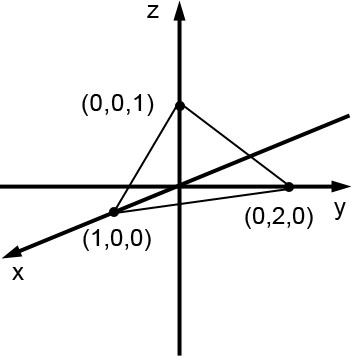
\includegraphics[width=0.35\textwidth]{ImgTetExample.jpg}
  \end{center}
\end{figure}
% ~  ~  ~  ~  ~  ~  ~  ~  ~  ~  ~  ~  ~  ~  ~  ~  ~  ~  ~  ~  ~  ~  ~  ~  
\item The tetrahedron has one side in the $xy$-plane. This side is bounded by the line that is the intersection between the $xy$-plane and the plane $z = 1 - x - y/2$. We can find this intersection by setting $z=0$,
\begin{align*}
  0 &= 1 - x - \frac{y}{2} \\
  x &= 1 - \frac{y}{2}.
\end{align*}
Therefore, the volume is the region under the plane $z = 1 - x - y/2$ and over  
\begin{align*}
  R = \{ (x,y) \ | \ 0 \le x \le 1- y/2, \ 0 \le y \le 2 \}.
\end{align*}
The double integral is 
\begin{align*}
  \mathop{\int_{0}^{2} \! \int_0^{1-y/2} } (1 - x - \frac{y}{2}) dxdy
\end{align*} 
% ~  ~  ~  ~  ~  ~  ~  ~  ~  ~  ~  ~  ~  ~  ~  ~  ~  ~  ~  ~  ~  ~  ~  ~  
\item The volume is the region under the plane $z = 1 - x - y/2$ and over  
\begin{align*}
  R = \{ (x,y) \ | \ 0 \le x \le 1, \ 0 \le y \le 2 - 2x \}.
\end{align*}
The double integral is 
\begin{align*}
  \mathop{\int_{0}^{1} \! \int_0^{2-2x} } (1 - x - \frac{y}{2}) dydx
\end{align*} 
\EEN
% ~~~~~~~~~~~~~~~~~~~~~~~~~~~~~~~~~~~~~~~~~~~~~~~~~~~~~~~~~~~~~~~~~~~~~~~~~~~~~~~~~
\item % DOUBLE INTEGRAL IS AREA IF F=1
\BEN
\item
Suppose that we subdivide region $R$ into a rectangular grid of sub-rectangles (as in Figure 3.2.5), so that we only consider the sub-rectangles that are completely enclosed in $R$. Then, the area of region $R$ is approximated by the double sum
\begin{align*}
  \sum_j\sum_i\Delta x_i \Delta y_j
\end{align*}
But if $f=1$ for all $x_i$ and $y_j$, this is equal to:
\begin{align}\label{abefaberabreabr}
  \sum_j\sum_i f(x_i,y_j) \Delta x_i \Delta y_j
\end{align}
where $x_i$ and $y_j$ is a point inside sub-rectangle $[x_i,x_{i+1}]\times[y_j,y_{j+1}]$. 
If we take smaller and smaller rectangles, so that the length of the longest diagonal of the sub-rectangles goes to zero, the sub-rectangles begin to fill more and more of the region $R$, and so the above sums approach the  \Emph{area} of region $R$. Since we have defined
\begin{align*}
  \mathop{\int \!\!\! \int} f(x,y) dA
\end{align*}
as the limit of Equation (\ref{abefaberabreabr}) as the longest diagonal goes to zero, and $f(x,y)=1$, the double integral 
\begin{align*}
  \mathop{\int \!\!\! \int} 1 dA
\end{align*}
is the area of region $R$. 
\item The region may be defined as
\begin{align*}
  R = \{ (x,y) \ | \ 0 \le x \le 1, \ x^2 \le y \le \sqrt{x} \}.
\end{align*}
The area of $R$ is 
\begin{align*}
  \mathop{\int_0^1 \!\!\! \int_{x^2}^{\sqrt{x}}} dydx 
  &= \int_0^1 \Big(\sqrt{x} - x^2 \Big) dx \\
  &= \Big(\frac{2}{3}x^{3/2}  - \frac{x^3}{3} \Big)\Big|_0^1 \\
  &= \frac{2}{3} - \frac{1}{3} \\
  &= \frac{1}{3}
\end{align*}
\EEN
% ~~~~~~~~~~~~~~~~~~~~~~~~~~~~~~~~~~~~~~~~~~~~~~~~~~~~~~~~~~~~~~~~~~~~~~~~~~~~~~~~~
\item % UPPER AND LOWER BOUNDS ARE FUNCTIONS
The curves $y=x^2$ and $x^2=y$ intersect at (0,0) and at (1,1). Integrating with respect to $y$ first yields
\begin{align*} 
  \mathop{\int_0^1 \!\!\! \int_{x^2}^{\sqrt{x}}} x^2+y^2 dydx 
  &= \int_0^1 \Big(yx^2 + \frac{y^3}{3} \Big)\Big|_{x^2}^{\sqrt{x}} dx \\
  &= \int_0^1 \Big(x^{5/2} + \frac{x^{3/2}}{3} - x^4 - \frac{x^6}{3}\Big) dx \\
  &= \Big( \frac{2}{7} x^{7/2} + \frac{2}{15}x^{5/2} - \frac{1}{5}x^5 - \frac{1}{21}x^7\Big)\Big|_0^1 \\
  &= \frac{2}{7} + \frac{2}{15} - \frac{1}{5} - \frac{1}{21} \\
  &= 6/35
\end{align*}
% ~~~~~~~~~~~~~~~~~~~~~~~~~~~~~~~~~~~~~~~~~~~~~~~~~~~~~~~~~~~~~~~~~~~~~~~~~~~~~~~~~
\item % CHANGING ORDER OF INTEGRATION
\BEN 
\item Integrating with respect to $y$ first yields
\begin{align*} 
  \mathop{\int_0^2 \!\!\! \int_0^{x^2}} x\sin (y) dydx 
  &= \int_0^2 -x\cos(y)\Big|_0^{x^2} dx \\
  &= - \int_0^2 \Big(x\cos(x^2)-1\Big) dx \\
  &= - \int_0^2x\cos(x^2) dx +  \int_0^2 1 \ dx \\    
  &= 2 - \int_0^2x\cos(x^2) dx 
\end{align*}
Now let $u=x^2$, so that $du = 2xdx$. Then 
\begin{align*} 
  2 - \int_0^2x\cos(x^2) dx  
  &=  2 - \int_0^4 x\cos(u)\Big(\frac{du}{2x}\Big)\\
  &=  2 - \frac{1}{2} \int_0^4 \cos(u)du \\
  &=  2 - \frac{1}{2} \sin(u) \Big|_0^4 \\
  &=  2 - \frac{1}{2} \sin(4) \\
  &\approx 2.3784
\end{align*}
\item Integrating with respect to $x$ first yields
\begin{align*} 
  \mathop{\int_0^4 \!\!\! \int_{\sqrt{y}}^{2} } x\sin (y) dxdy
  &= \int_0^4 \frac{x^2}{2}\sin(y)\Big|_{\sqrt{y}}^{2} \ dy \\
  &= \int_0^4 \frac{4-y}{2}\sin(y) dy \\
  &= 2 \int_0^4 \sin(y) dy - \frac{1}{2} \int_0^4 y\sin(y) dy \\
  &= 2 \big( - \cos(y) \big)\big|_0^4 - \frac{1}{2} \int_0^4 y\sin(y) dy \\
  &= 2 \big( - \cos(4) + 1 \big) - \frac{1}{2} \int_0^4 y\sin(y) dy \\
  &= 2  - 2\cos(4)  - \frac{1}{2} \int_0^4 y\sin(y) dy \\
\end{align*}
Now using integration by parts, with 
\begin{align*}
  u &= y, \quad dv = \sin(y)dy \\
  du &= dy, \quad v = -\cos(y)
\end{align*}
we obtain
\begin{align*} 
  \mathop{\int_0^4 \!\!\! \int_{\sqrt{y}}^{2} } x\sin (y) dxdy
  &= 2  - 2\cos(4)  - \frac{1}{2} \int_0^4 y\sin(y) dy \\
  &= 2  - 2\cos(4)  - \frac{1}{2}\Bigg( -y\cos(y)\Big|_0^4 - \int_0^4 \big(-\cos(y)\big) dy \Bigg) \\
  &= 2  - 2\cos(4)  - \frac{1}{2}\Bigg( -4\cos4 + \sin(y)\big|_0^4 \Bigg)  \\  
  &= 2  - 2\cos(4)  - \frac{1}{2}\Big( -4\cos4 + \sin(4)- 0 \Big)  \\  
  &= 2 - \frac{\sin(4)}{2}   \\  
  &\approx 2.3784
\end{align*}
\EEN
% ~~~~~~~~~~~~~~~~~~~~~~~~~~~~~~~~~~~~~~~~~~~~~~~~~~~~~~~~~~~~~~~~~~~~~~~~~~~~~~~~~
\item % CHANGING ORDER OF INTEGRATION, GENERAL F(X,Y)
The region over which we are integrating $f(x,y)$ is the shaded area below. 
\begin{figure}[h]
  \vspace{-1pt}
  \begin{center}
    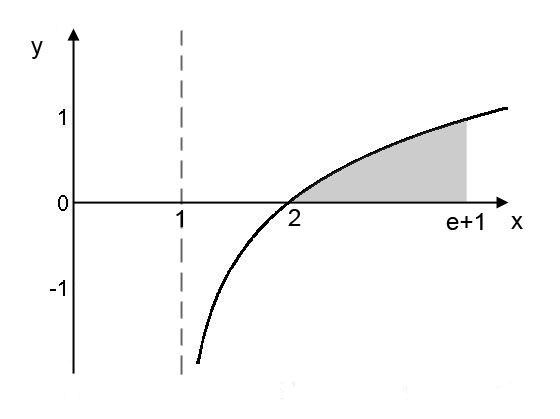
\includegraphics[width=0.55\textwidth]{ImgLog.jpg}
  \end{center}
\end{figure}\\
The region is bounded by the lines $y=0$, $x=1+e$, and by the curve $y=\ln(x-1)$. Using horizontal slices, values of $y$ range from 0 to 1, and values of $x$ range from $e^y-1$ to $1+e$. The double integral becomes
\begin{align*}
  \mathop{\int_{0}^{1} \! \int_{e^y-1}^{1+e}} f(x,y) dydx .
\end{align*}
% ~~~~~~~~~~~~~~~~~~~~~~~~~~~~~~~~~~~~~~~~~~~~~~~~~~~~~~~~~~~~~~~~~~~~~~~~~~~~~~~~~
\item % BOUNDING AN INTEGRAL 
The integrand $f(x,y)$ has the property that 
\begin{align*}
  0 \le \sin(x+y) \le 1,
\end{align*}
because $x+y$ is between 0 and 2, and $\sin(2) < 1$. Then 
\begin{align*}
  0 = \iint\limits_D 0 dA  \le  \iint\limits_D f(x,y) dA \le  \iint\limits_D (1) dA = 1.
\end{align*}
% ~~~~~~~~~~~~~~~~~~~~~~~~~~~~~~~~~~~~~~~~~~~~~~~~~~~~~~~~~~~~~~~~~~~~~~~~~~~~~~~~~
\item % SYMMETRY
\BEN
\item 
Suppose we use the function
\begin{align*}
 h(x,y) & = 11xy.
\end{align*}
Then $h(-x,y) = 11(-x)y = -11xy = -h(x,y)$. 
\item An example of a region that is symmetric about the $y$-axis, but not symmetric about the $x$-axis, is the region bounded by the curves
\begin{align*}
  x = -1,  \quad x = 1, \quad y = 0, \quad y = - 1.
\end{align*}
\item The double integral for our region is
\begin{align*}
  \iint\limits_D g(x,y) dxdy 
  &=  \mathop{\int_{-1}^1 \! \int_{-1}^0} 11xy dydx\\
  &=  -\frac{11}{2} \int_{-1}^1 x dx\\
  &=  -\frac{11}{4} \Big(x^2 \Big)\Big|_{-1}^{1} \\
  &=  -\frac{11}{4} (0)\\
  &= 0.
\end{align*}
\EEN
% ~~~~~~~~~~~~~~~~~~~~~~~~~~~~~~~~~~~~~~~~~~~~~~~~~~~~~~~~~~~~~~~~~~~~~~~~~~~~~~~~~
\EEN % END OF SOLUTIONS
\newpage
% s~s~s~s~s~s~s~s~s~s~s~s~s~s~s~s~s~s~s~s~s~s~s~s~s~s~s~s~s~s~s~s~s~s~s~s~s~s~s~s~s~s~s~s
% s~s~s~s~s~s~s~s~s~s~s~s~s~s~s~s~s~s~s~s~s~s~s~s~s~s~s~s~s~s~s~s~s~s~s~s~s~s~s~s~s~s~s~s
\subsection{Triple Integrals}

\BEN
% ~~~~~~~~~~~~~~~~~~~~~~~~~~~~~~~~~~~~~~~~~~~~~~~~~~~~~~~~~~~~~~~~~~~~~~~~~~~~~~~~~
\item % TETRAHEDRON
\Emph{Volume of a Tetrahedron} \\
\begin{figure}[h]
  \vspace{-1pt}
  \begin{center}
    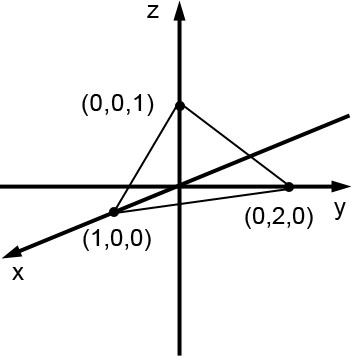
\includegraphics[width=0.35\textwidth]{ImgTetExample.jpg}
  \end{center}
\end{figure}\\
Recall that the volume is the region under the plane $z = 1 - x - y/2$ and over  
\begin{align*}
  R = \{ (x,y) \ | \ 0 \le x \le 1- y/2, \ 0 \le y \le 2 \}.
\end{align*}
Because $z$ lies between 0 and $z = 1 - x - y/2$, the volume, $S$, can be described as
\begin{align*}
  S = \{ (x,y,z) \ | \ 0 \le x \le 1- y/2, \ 0 \le y \le 2, \ 0 \le z \le 1 - x - y/2 \}.
\end{align*}
The volume can be calculated with the triple integral
\begin{align*}
  \mathop{\int_{0}^{2} \! \int_0^{1-y/2} \int_0^{1-x-y/2} }dzdxdy
  &= \mathop{\int_{0}^{2} \! \int_0^{1-y/2}  } ( 1-x-y/2) dxdy\\
  &= \mathop{\int_{0}^{2}  } \Big( x-\frac{x^2}{2}-\frac{xy}{2}\Big)\Big|_0^{1-y/2} dy \\
  &= \mathop{\int_{0}^{2}  } \Big( (1-y/2)-\frac{(1-y/2)^2}{2}-\frac{(y-y^2/2)}{2}\Big) dy \\
  &= \mathop{\int_{0}^{2}  } \Bigg( 1 - \frac{y}{2}-\frac{1}{2}\Big(1 - y + \frac{y^2}{4}\Big)-\frac{y}{2}+\frac{y^2}{4}\Bigg) dy \\
  &= \mathop{\int_{0}^{2}  } \Bigg( 1 - \frac{y}{2} - \frac{1}{2} + \frac{y}{2} - \frac{y^2}{8} -\frac{y}{2}+\frac{y^2}{4}\Bigg) dy \\
  &= \mathop{\int_{0}^{2}  } \Big( \frac{1}{2} - \frac{y}{2} + \frac{y^2}{8} \Big) dy \\
  &= \frac{2}{2} - \frac{4}{4}  + \frac{8}{24} \\
  &= \frac{1}{3}
\end{align*} 
% ~~~~~~~~~~~~~~~~~~~~~~~~~~~~~~~~~~~~~~~~~~~~~~~~~~~~~~~~~~~~~~~~~~~~~~~~~~~~~~~~~
\item % VOLUME OF AN ELLIPSOID
\textbf{Volume of an Ellipsoid}\\
We are given the transformations  
\begin{align*}
  x=au, \quad y=bv, \quad z=cw.
\end{align*}
The Jacobian becomes 
\begin{align*}   J &=  
  \begin{vmatrix}
   \pxu &  \pxv & \pxw \\\\
   \pyu & \pyv & \pyw \\\\
   \pzu & \pzv & \pzw 
  \end{vmatrix}
  =     
  \begin{vmatrix}
 a&0&0\\
 0&b&0\\
 0&0&c\\
  \end{vmatrix}
  = abc.
 \end{align*}
 The solid enclosed by the ellipsoid is the image of the unit sphere $u^2 + v^2 + w^2 \le 1$. Using that a sphere has volume $\frac{4}{3} \pi r^3$, we find that 
\begin{align*}
  \iiint\limits_{V} dxdydz
  &=  \iiint\limits_{u^2+v^2+w^2 \le 1} abc \ dudvdw \\
  &=  abc \iiint\limits_{u^2+v^2+w^2 \le 1} \ dudvdw \\
  &=  abc (\text{volume of a sphere}) \\
  &=   \frac{4\pi abc}{3} 
\end{align*}

% ~~~~~~~~~~~~~~~~~~~~~~~~~~~~~~~~~~~~~~~~~~~~~~~~~~~~~~~~~~~~~~~~~~~~~~~~~~~~~~~~~
\item % CHANGING ORDER OF INTEGRATION
\textbf{Changing the Order of Integration}\\
% ~~~~~~~~~~~~~~~~~~~~~~~~~~~~~~~~~~~~~~~~~~~~~~~~~~~~~~~~~~~~~~~~~~~~~~~~~~~~~~~~~
\EEN % END OF SUBSECTION
% s~s~s~s~s~s~s~s~s~s~s~s~s~s~s~s~s~s~s~s~s~s~s~s~s~s~s~s~s~s~s~s~s~s~s~s~s~s~s~s~s~s~s~s
% s~s~s~s~s~s~s~s~s~s~s~s~s~s~s~s~s~s~s~s~s~s~s~s~s~s~s~s~s~s~s~s~s~s~s~s~s~s~s~s~s~s~s~s
\subsection{Change of Variables in Multiple Integrals}

\BEN
% ~~~~~~~~~~~~~~~~~~~~~~~~~~~~~~~~~~~~~~~~~~~~~~~~~~~~~~~~~~~~~~~~~~~~~~~~~~~~~~~~~
\item % GENERAL LINEAR TRANSFORMATION
\Emph{Linear Transformations} \\
\BEN
\item Substituting $v = v_0$ into the linear transformation yields the two equations
\begin{align*}
  x &= c_1u + c_2v_0 \\ 
  y &= d_1u + d_2v_0
\end{align*}
To find the equation of the line in the $xy$-plane, we need to eliminate $u$. There are many ways to do this, but let's multiply the first equation by $d_1$ and the second by $c_1$.
\begin{align*}
  d_1x &= c_1d_1u + c_2d_1v_0 \\ 
  c_1y &= c_1d_1u + d_2c_1v_0
\end{align*}
Subtracting these equations yields
\begin{align*}
  d_1x -  c_1y &=  (c_2d_1 -  d_2c_1)v_0 
\end{align*}
A simple rearrangement gives us
\begin{align*}
  c_1y &= d_1x - (c_2d_1 -  d_2c_1)v_0 .
\end{align*}
Provided that $c_1$ is not zero, we could write this in the form
\begin{align*}
  y &= \frac{d_1}{c_1}x - \frac{c_2d_1 -  d_2c_1}{c_1}v_0 .
\end{align*}
% ~  ~  ~  ~  ~  ~  ~  ~  ~  ~  ~  ~  ~  ~  ~  ~  ~  ~  ~  ~  ~  ~  ~  ~  ~  ~  ~  ~
\item Substituting $x=x_0$ into $x =c_1u + c_2v$ gives us 
\begin{align*}
  x_0 &= c_1u + c_2v,
\end{align*}
Provided that $c_2$ is not zero, 
This is the is mapped into the $uv$-plane REWORD
\EEN

% ~~~~~~~~~~~~~~~~~~~~~~~~~~~~~~~~~~~~~~~~~~~~~~~~~~~~~~~~~~~~~~~~~~~~~~~~~~~~~~~~~
\item % STRAIGHTFORWARD CHANGE OF VARIABLES
The integral can be written as
\begin{align*}
  \iint\limits_R \big(x^2 - y^2\big) dxdy =  \iint\limits_R (x - y)(x+y) dxdy.
\end{align*}
Recall that $R$ is the region bounded by
\begin{align*}
  x+y = 0, \quad x+y = 1, \quad x-y=0, \quad x-y=1.
\end{align*}
The appearance of the terms $(x+y)$ and $(x - y)$ in the integrand and in the lines that bound $R$ suggests the transformation 
\begin{align}
  u & = x+y  \label{zcvzcxvvad}\\
  v &= x - y \label{ntrsraaewvbernst}.
\end{align}
In order to compute the Jacobian, we need explicit expressions for $u$ and $v$. If we add  equations \ref{zcvzcxvvad} and \ref{ntrsraaewvbernst} we find that 
\begin{align*}   x = \frac{u+v}{2}   \end{align*}
And if we subtract equations \ref{zcvzcxvvad} and \ref{ntrsraaewvbernst} we find that
\begin{align*}   y = \frac{u-v}{2}   \end{align*}
The Jacobian becomes
\begin{align*}   J &=  
  \begin{vmatrix}
   \pxu &  \pxv \\ \\
   \pyu & \pyv \\
  \end{vmatrix}
  =     \begin{vmatrix}
 \frac{1}{2} &  \frac{1}{2} \\ \\
   \frac{1}{2} & -\frac{1}{2} \\
  \end{vmatrix}
  = - \frac{1}{4}- \frac{1}{4} = - \frac{1}{2}.
 \end{align*}
We also need to find the limits of  integration in the transformed integral. Using equations \ref{zcvzcxvvad} and \ref{ntrsraaewvbernst} the four lines bounding $R$ in the $xy$-plane become 
\begin{align*}
  u = 0, \quad u = 1, \quad v=0, \quad v=1.
\end{align*}
The double integral therefore becomes
\begin{align*}
  \iint\limits_R \big(x^2 - y^2\big) dxdy 
  &=  \iint\limits_R (x - y)(x+y) dxdy \\
  &=    \mathop{\int_0^1 \! \int_0^1} uv \Bigg|-\frac{1}{2} \Bigg| dudv \\
  &=     \frac{1}{2}\mathop{\int_0^1 \! \int_0^1} (uv) dudv \\
  &=     \frac{1}{2}\int_0^1 \frac{v}{2} dv \\
  &=   \frac{1}{8}.
\end{align*}
% ~~~~~~~~~~~~~~~~~~~~~~~~~~~~~~~~~~~~~~~~~~~~~~~~~~~~~~~~~~~~~~~~~~~~~~~~~~~~~~~~~
\item % CHANGE OF VARIABLES TWICE WITH POLAR
The Jacobian is
\begin{align*}   J &=  
  \begin{vmatrix}
   \pxu &  \pxv \\ \\
   \pyu & \pyv \\
  \end{vmatrix}
  =     \begin{vmatrix}
   3 & 0 \\ \\
   0 & 2 \\
  \end{vmatrix}
  = 6 .
 \end{align*}
We also need to find the limits of integration in the transformed integral. The region $R$ is bounded by the ellipse, $4x^2 + 9y^2 = 36$, which becomes the region bounded by the circle $u^2 + v^2 = 1$. Therefore
\begin{align*}
  \iint\limits_R x^2 \ dxdy &= \iint\limits_{u^2 + v^2 \le 1} (9u^2) 6dudv =  54 \iint\limits_{u^2 + v^2 \le 1} (u^2) dudv
\end{align*}
Switching to polar coordinates, 
\begin{align*}
  u = r\cos\theta, \quad v = r\sin\theta, \quad J = r
\end{align*}
our double integral becomes
\begin{align*}
  54 \iint\limits_{u^2 + v^2 \le 1} (u^2) dudv 
  & = 54 \mathop{\int_0^{2\pi} \!\! \int_0^1} r^3\cos^2\theta drd\theta  \\
  & = 54 \Bigg( \int_0^{2\pi} \cos^2\theta d\theta \Bigg)\Bigg( \int_0^1 r^3 dr \Bigg) \\
  & = 54 \Bigg( \int_0^{2\pi} \frac{1}{2} \big(1+\cos(2\theta) \big) d\theta \Bigg) \Bigg( \frac{1}{4} \Bigg) \\
  & =\frac{27}{4} \Bigg( \int_0^{2\pi}  \big(1+\cos(2\theta) \big) d\theta \Bigg) \\
  & =\frac{27}{4} \big(\theta+\frac{1}{2}\sin(2\theta) \big|_0^{2\pi}  \\
  & =\frac{27}{4} \big(2\pi\big)  \\
  & =\frac{27\pi}{2} 
\end{align*}
% ~~~~~~~~~~~~~~~~~~~~~~~~~~~~~~~~~~~~~~~~~~~~~~~~~~~~~~~~~~~~~~~~~~~~~~~~~~~~~~~~~
\item % SIMPLE CYLINDRICAL WITH CONE
In cylindrical coordinates, the region is described by 
\begin{align*}
  V = \{(r,\theta,z) \ | \ 0 \le r \le 1, 0 \le \theta \le 2\pi, 0 \le z \le 3r \}.
\end{align*}
Our integral becomes 
\begin{align*}
  \iiint\limits_V (r\sin\theta)^2 rdzdrd\theta 
  &=    \mathop{\int_0^{2\pi} \!\! \int_0^1  \!\! \int_0^{3r}} r^3\sin^2\theta dzdrd\theta  \\
  &=   3 \mathop{\int_0^{2\pi} \!\! \int_0^1} r^4\sin^2\theta drd\theta  \\
  &=   \frac{3}{5} \int_0^{2\pi} \sin^2\theta d\theta  \\
  &=   \frac{3}{10} \int_0^{2\pi} \big(1 - \cos(2\theta)\big) d\theta  \\
  &=   \frac{3}{10} \big(\theta - \frac{1}{2}\sin(2\theta)\big) \Big|_0^{2\pi} \\
  &=   \frac{3\pi}{5}
\end{align*}
% ~~~~~~~~~~~~~~~~~~~~~~~~~~~~~~~~~~~~~~~~~~~~~~~~~~~~~~~~~~~~~~~~~~~~~~~~~~~~~~~~~
\item % TRIPLE INTEGRAL IN CYLINDRICAL COORDINATES
In cylindrical coordinates,  $V$ is the region bounded by
\begin{align*}
  0 \le\ &r \le 2 \\
  0 \le\ &\theta \le \frac{\pi}{2}\\
  0 \le\ &z \le \sqrt{4 - r^2}
\end{align*}
The triple integral becomes
\begin{align*}
  \iiint\limits_V dxdydz
  &=    \mathop{\int_0^{\pi/2} \!\! \int_0^2  \!\! \int_0^{\sqrt{4 - r^2}}} r dzdrd\theta  \\
  &=    \mathop{\int_0^{\pi/2} \!\! \int_0^2 } r\sqrt{4 - r^2}drd\theta  \\
  &=   \frac{-1}{3} \int_0^{\pi/2} (4 - r^2)^{3/2} \Big|_0^2 d\theta  \\
  &=   \frac{-1}{3} \int_0^{\pi/2} (0 - 8) d\theta  \\
  &=   \frac{4\pi}{3}
\end{align*}
% ~~~~~~~~~~~~~~~~~~~~~~~~~~~~~~~~~~~~~~~~~~~~~~~~~~~~~~~~~~~~~~~~~~~~~~~~~~~~~~~~~
\item % TRIPLE INTEGRAL IN SPHERICAL COORDINATES
\Emph{Triple Integral In Spherical Coordinates} \\
The solid is a section of a sphere with radius 1, centered at the origin. The section is the part of the sphere that lies above the plane $z=0$, and between the planes $y=0$, and $y=x$. 
\begin{align*}
  \mathop{\int_0^{\pi/4} \!\! \int_{0}^{\pi/2} \!\! \int_0^1 } ( \rho^2 \sin\phi ) \ d\rho\  d\phi\  d\theta
  &=   \mathop{\int_0^{\pi/4} \!\! \int_{0}^{\pi/2} }  \frac{ \sin\phi}{3}  d\phi\  d\theta\\
  &=   \int_0^{\pi/4} \frac{-(0-1)}{3}   d\theta \\
  &=  \pi/12
\end{align*}
% ~~~~~~~~~~~~~~~~~~~~~~~~~~~~~~~~~~~~~~~~~~~~~~~~~~~~~~~~~~~~~~~~~~~~~~~~~~~~~~~~~
\EEN % END OF SUBSECTION
% s~s~s~s~s~s~s~s~s~s~s~s~s~s~s~s~s~s~s~s~s~s~s~s~s~s~s~s~s~s~s~s~s~s~s~s~s~s~s~s~s~s~s~s
% s~s~s~s~s~s~s~s~s~s~s~s~s~s~s~s~s~s~s~s~s~s~s~s~s~s~s~s~s~s~s~s~s~s~s~s~s~s~s~s~s~s~s~s
\subsection{Application: Center of Mass}
\BEN
% ~~~~~~~~~~~~~~~~~~~~~~~~~~~~~~~~~~~~~~~~~~~~~~~~~~~~~~~~~~~~~~~~~~~~~~~~~~~~~~~~~
\item % CENTER OF MASS OF 2D TRIANGULAR PLATE
\Emph{Center of Mass of a 2D Triangular Plate} \\
The total mass of the plate is
\begin{align*}
  M 
  &= \iint\limits_R \delta(x,y) dA \\
  &=    \mathop{\int_0^1 \!\! \int_{2x}^{4x} } xy \ dydx \\
  &=  \frac{1}{2}  \int_0^1 x(16x^2 - 4x^2) \ dx \\
  &= 6  \int_0^1 x^3 \ dx \\
  &=   \frac{3}{2}.
\end{align*}

The $x$-coordinate of the center of mass is
\begin{align*}
  \bar{x} = \frac{M_y}{M} 
  &= \frac{2}{3} \iint\limits_R x \delta(x,y) dA \\
  &=    \mathop{\int_0^1 \!\! \int_{2x}^{4x} } x^2y \ dydx \\
  &=  \frac{1}{2}  \int_0^1 x^2(16x^2 - 4x^2) \ dx \\
  &= 6  \int_0^1 x^4 \ dx \\
  &=   \frac{6}{5}.
\end{align*}

The $y$-coordinate of the center of mass is
\begin{align*}
  \bar{y} = \frac{M_x}{M} 
  &= \frac{2}{3} \iint\limits_R y \delta(x,y) dA \\
  &=    \mathop{\int_0^1 \!\! \int_{2x}^{4x} } xy^2 \ dydx \\
  &=  \frac{1}{3}  \int_0^1 x(64x^3 - 8x^3) \ dx \\
  &=  \frac{56}{3}  \int_0^1 x^4 \ dx \\
  &=   \frac{56}{15}.
\end{align*}
Thus, the coordinates of the center of mass are $(6/5,56/15)$.
% ~~~~~~~~~~~~~~~~~~~~~~~~~~~~~~~~~~~~~~~~~~~~~~~~~~~~~~~~~~~~~~~~~~~~~~~~~~~~~~~~~
\item % CENTER OF MASS OF 2D RADIAL DENSITY FUNCTION
\Emph{Center of Mass of a 2D Plate, Radial Density Function} \\
We could express the coordinates of the center of mass using either Cartesian or polar coordinates. Using Cartesian coordinates, the density, $\delta$, at point $(x,y)$, is given by
\begin{align*}
  \delta(x,y) = L(x,y) = a - \sqrt{x^2+y^2}.
\end{align*}
\BEN
\item
The $x$-coordinate of the center of mass is
\begin{align*}
  \bar{x} = \frac{M_y}{M} 
  = \frac{1}{M} \iint\limits_R x \delta(x,y) dA 
  = \frac{1}{M}  \mathop{\int_{-a}^{a} \!\! \int_{0}^{\sqrt{x^2+y^2}}} x\Big( a - \sqrt{x^2+y^2}\Big) \ dydx 
\end{align*}
\item
The $y$-coordinate of the center of mass is
\begin{align*}
  \bar{y} = \frac{M_x}{M} 
  = \frac{1}{M} \iint\limits_R y \delta(x,y) dA 
  = \frac{1}{M}  \mathop{\int_{-a}^{a} \!\! \int_{0}^{\sqrt{x^2+y^2}}} y\Big( a - \sqrt{x^2+y^2}\Big) \ dydx 
\end{align*}
\item The center of mass is located on the $y$-axis. In other words, $\bar{x}=0$. This is because of symmetry: the integrand of $\bar{x}$ is odd in $x$, the integral with respect to $x$ is calculated about an interval that is symmetric about the $y$-axis, and so the integral with respect to $x$ is zero. 
\EEN
Note that we could just as easily set up the above integrals using polar coordinates. The 2D circular plate, in polar coordinates, is bounded by 
\begin{align*}
  0 \le r \le a, \quad 0 \le \theta \le \pi, \quad a > 0.
\end{align*}
The coordinates for the center of mass are
\begin{align*}
  \bar{x} &= \frac{M_y}{M} 
  = \frac{1}{M} \iint\limits_R x \delta(x,y) dA 
  = \frac{1}{M}  \mathop{\int_{0}^{\pi} \!\! \int_{0}^r} r\cos(\theta) ( a - r ) \ rdrd\theta \\
  \bar{y} &= \frac{M_x}{M} 
  = \frac{1}{M} \iint\limits_R y \delta(x,y) dA 
  = \frac{1}{M}  \mathop{\int_{0}^{\pi} \!\! \int_{0}^r} r\sin(\theta) ( a -r ) \ rdrd\theta
\end{align*}
 
% ~~~~~~~~~~~~~~~~~~~~~~~~~~~~~~~~~~~~~~~~~~~~~~~~~~~~~~~~~~~~~~~~~~~~~~~~~~~~~~~~~
\item % EVEN AND ODD
The integral can be written as
\begin{align*}
  \mathop{\int_0^{\pi} \!\! \int_{-1}^1} e^{x^2 + y^2}\sin(y) dydx 
  &= \mathop{\int_0^{\pi} \!\! \int_{-1}^1} e^{x^2}e^{y^2}\sin(y) dydx  = \Bigg( \int_0^{\pi} e^{x^2} dx \Bigg)\Bigg( \int_{-1}^1 e^{y^2}\sin(y)dy \Bigg)  
\end{align*}
The second term is the integral of an odd function over a symmetrical interval, and so is equal to zero. Therefore,
\begin{align*}
  \mathop{\int_0^{\pi} \!\! \int_{-1}^1} e^{x^2 + y^2}\sin(y) dydx =0.
\end{align*}

% ~~~~~~~~~~~~~~~~~~~~~~~~~~~~~~~~~~~~~~~~~~~~~~~~~~~~~~~~~~~~~~~~~~~~~~~~~~~~~~~~~
\EEN % END OF SOLUTIONS


\end{document}
